% Options for packages loaded elsewhere
% Options for packages loaded elsewhere
\PassOptionsToPackage{unicode}{hyperref}
\PassOptionsToPackage{hyphens}{url}
%
\documentclass[
  10pt,
  a4paper,
]{scrbook}
\usepackage{xcolor}
\usepackage[left=2.54cm,right=2.54cm]{geometry}
\usepackage{amsmath,amssymb}
\setcounter{secnumdepth}{2}
\usepackage{iftex}
\ifPDFTeX
  \usepackage[T1]{fontenc}
  \usepackage[utf8]{inputenc}
  \usepackage{textcomp} % provide euro and other symbols
\else % if luatex or xetex
  \usepackage{unicode-math} % this also loads fontspec
  \defaultfontfeatures{Scale=MatchLowercase}
  \defaultfontfeatures[\rmfamily]{Ligatures=TeX,Scale=1}
\fi
\usepackage{lmodern}
\ifPDFTeX\else
  % xetex/luatex font selection
\fi
% Use upquote if available, for straight quotes in verbatim environments
\IfFileExists{upquote.sty}{\usepackage{upquote}}{}
\IfFileExists{microtype.sty}{% use microtype if available
  \usepackage[]{microtype}
  \UseMicrotypeSet[protrusion]{basicmath} % disable protrusion for tt fonts
}{}
\usepackage{setspace}
\makeatletter
\@ifundefined{KOMAClassName}{% if non-KOMA class
  \IfFileExists{parskip.sty}{%
    \usepackage{parskip}
  }{% else
    \setlength{\parindent}{0pt}
    \setlength{\parskip}{6pt plus 2pt minus 1pt}}
}{% if KOMA class
  \KOMAoptions{parskip=half}}
\makeatother
% Make \paragraph and \subparagraph free-standing
\makeatletter
\ifx\paragraph\undefined\else
  \let\oldparagraph\paragraph
  \renewcommand{\paragraph}{
    \@ifstar
      \xxxParagraphStar
      \xxxParagraphNoStar
  }
  \newcommand{\xxxParagraphStar}[1]{\oldparagraph*{#1}\mbox{}}
  \newcommand{\xxxParagraphNoStar}[1]{\oldparagraph{#1}\mbox{}}
\fi
\ifx\subparagraph\undefined\else
  \let\oldsubparagraph\subparagraph
  \renewcommand{\subparagraph}{
    \@ifstar
      \xxxSubParagraphStar
      \xxxSubParagraphNoStar
  }
  \newcommand{\xxxSubParagraphStar}[1]{\oldsubparagraph*{#1}\mbox{}}
  \newcommand{\xxxSubParagraphNoStar}[1]{\oldsubparagraph{#1}\mbox{}}
\fi
\makeatother


\usepackage{longtable,booktabs,array}
\newcounter{none} % for unnumbered tables
\usepackage{calc} % for calculating minipage widths
% Correct order of tables after \paragraph or \subparagraph
\usepackage{etoolbox}
\makeatletter
\patchcmd\longtable{\par}{\if@noskipsec\mbox{}\fi\par}{}{}
\makeatother
% Allow footnotes in longtable head/foot
\IfFileExists{footnotehyper.sty}{\usepackage{footnotehyper}}{\usepackage{footnote}}
\makesavenoteenv{longtable}
\usepackage{graphicx}
\makeatletter
\newsavebox\pandoc@box
\newcommand*\pandocbounded[1]{% scales image to fit in text height/width
  \sbox\pandoc@box{#1}%
  \Gscale@div\@tempa{\textheight}{\dimexpr\ht\pandoc@box+\dp\pandoc@box\relax}%
  \Gscale@div\@tempb{\linewidth}{\wd\pandoc@box}%
  \ifdim\@tempb\p@<\@tempa\p@\let\@tempa\@tempb\fi% select the smaller of both
  \ifdim\@tempa\p@<\p@\scalebox{\@tempa}{\usebox\pandoc@box}%
  \else\usebox{\pandoc@box}%
  \fi%
}
% Set default figure placement to htbp
\def\fps@figure{htbp}
\makeatother


% definitions for citeproc citations
\NewDocumentCommand\citeproctext{}{}
\NewDocumentCommand\citeproc{mm}{%
  \begingroup\def\citeproctext{#2}\cite{#1}\endgroup}
\makeatletter
 % allow citations to break across lines
 \let\@cite@ofmt\@firstofone
 % avoid brackets around text for \cite:
 \def\@biblabel#1{}
 \def\@cite#1#2{{#1\if@tempswa , #2\fi}}
\makeatother
\newlength{\cslhangindent}
\setlength{\cslhangindent}{1.5em}
\newlength{\csllabelwidth}
\setlength{\csllabelwidth}{3em}
\newenvironment{CSLReferences}[2] % #1 hanging-indent, #2 entry-spacing
 {\begin{list}{}{%
  \setlength{\itemindent}{0pt}
  \setlength{\leftmargin}{0pt}
  \setlength{\parsep}{0pt}
  % turn on hanging indent if param 1 is 1
  \ifodd #1
   \setlength{\leftmargin}{\cslhangindent}
   \setlength{\itemindent}{-1\cslhangindent}
  \fi
  % set entry spacing
  \setlength{\itemsep}{#2\baselineskip}}}
 {\end{list}}
\usepackage{calc}
\newcommand{\CSLBlock}[1]{\hfill\break\parbox[t]{\linewidth}{\strut\ignorespaces#1\strut}}
\newcommand{\CSLLeftMargin}[1]{\parbox[t]{\csllabelwidth}{\strut#1\strut}}
\newcommand{\CSLRightInline}[1]{\parbox[t]{\linewidth - \csllabelwidth}{\strut#1\strut}}
\newcommand{\CSLIndent}[1]{\hspace{\cslhangindent}#1}



\setlength{\emergencystretch}{3em} % prevent overfull lines

\providecommand{\tightlist}{%
  \setlength{\itemsep}{0pt}\setlength{\parskip}{0pt}}



 


% Palatino font:
\usepackage[T1]{fontenc}
\usepackage[utf8]{inputenc}
\usepackage{palatino}

\usepackage{ragged2e}

%\usepackage{mathpazo}
\usepackage{newpxtext}
\usepackage{newpxmath}

\usepackage{upquote}

% % let latex break paragraphs to fill pages
% \clubpenalty=0
% \widowpenalty=0
% \displaywidowpenalty=0
% \interlinepenalty=0
% \brokenpenalty=0
% \flushbottom

% make sure floats stay in sections
\usepackage[section]{placeins}

\usepackage{newunicodechar}
\newunicodechar{θ}{\ensuremath{\theta}}
\newunicodechar{π}{\ensuremath{\pi}}
\newunicodechar{μ}{\ensuremath{\mu}}
\newunicodechar{₀}{\ensuremath{_0}}
\newunicodechar{₁}{\ensuremath{_1}}
\newunicodechar{₂}{\ensuremath{_2}}
\newunicodechar{ₑ}{\ensuremath{_e}}
\newunicodechar{×}{\ensuremath{\times}}
\newunicodechar{≈}{\ensuremath{\approx}}
\newunicodechar{≤}{\ensuremath{\leq}}
\newunicodechar{≥}{\ensuremath{\geq}}
\newunicodechar{⁻}{\ensuremath{^{-}}}
\newunicodechar{⁸}{\ensuremath{^{8}}}
\newunicodechar{̂}{\^{}}
\usepackage{float}
\newunicodechar{τ}{\ensuremath{\tau}}
\newunicodechar{₃}{\ensuremath{_3}}
\newunicodechar{₄}{\ensuremath{_4}}
\newunicodechar{₅}{\ensuremath{_5}}
\newunicodechar{₆}{\ensuremath{_6}}
\newunicodechar{₇}{\ensuremath{_7}}
\newunicodechar{₈}{\ensuremath{_8}}
\newunicodechar{₉}{\ensuremath{_9}}
\newunicodechar{ₖ}{\ensuremath{_k}}
\newunicodechar{ₙ}{\ensuremath{_n}}
\newunicodechar{ₛ}{\ensuremath{_s}}
\newunicodechar{±}{\ensuremath{\pm}}
\newunicodechar{·}{\ensuremath{\cdot}}
\newunicodechar{σ}{\ensuremath{\sigma}}
\newunicodechar{ρ}{\ensuremath{\rho}}

% front page
\usepackage[colorlinks]{hyperref} % for text color on title
\usepackage{titling} % makes \thetitle etc available...
\usepackage{lipsum}
\usepackage{tikz}
\tikzstyle{bag} = [align=center] % allows new lines in text below
\AtBeginDocument{\thispagestyle{empty}
\definecolor{titlecolor}{HTML}{1C2404}
\begin{tikzpicture}[remember picture,overlay]
\draw (current page.center) node[inner sep=0] {\resizebox{!}{350mm}{\includegraphics{highres_banner.pdf}}};
\draw (current page.center) node[inner sep=0, opacity=0.5] {\resizebox{!}{100mm}{\includegraphics{ausegl_sort.pdf}}};
\draw (17, 2.7) node[bag, align=right, anchor=north east, text width=15cm] {%
    \hyphenpenalty=10000\exhyphenpenalty=10000%
    \color{titlecolor} \Large \textbf{Thesis} \\
    \color{titlecolor} \huge \textbf{\thetitle} \\
    \vspace{5 mm}
    \color{titlecolor} \Large \textbf{\theauthor} \\
    \vspace{3 mm}
    \color{titlecolor} \large \textbf{\thedate}
};
\end{tikzpicture}
\clearpage}

% back side
\AtEndDocument{\clearpage\thispagestyle{empty}
\begin{tikzpicture}[remember picture,overlay]
\draw (current page.center) node[inner sep=0] {\resizebox{!}{350mm}{\includegraphics{highres_banner.pdf}}};
    \draw (17, 1.7) node[bag, align=right, anchor=north east] {
        \color{titlecolor} \large Bioinformatics Research Centre \\
        \color{titlecolor} \large Department of Molecular Biology and Genetics \\
        \color{titlecolor} \large Aarhus University \\
        \color{titlecolor} \large Universitetsbyen 81 \\
        \color{titlecolor} \large 8000 Aarhus C \\
        \color{titlecolor} \large Denmark
        };
\end{tikzpicture}}


\usepackage[many]{tcolorbox}
\definecolor{quotegray}{HTML}{505050}
\newtcolorbox{myquote}{%
    enhanced jigsaw,
    breakable,
    frame hidden,
    left=1cm,
    right=1cm,
    colback=white,
    fontupper=\color{quotegray},
    overlay={%
        \node [scale=4,
            text=lightgray,
            inner sep=0pt,] at ([xshift=0.5cm,yshift=-0.7cm]frame.north west){``};
        \node [scale=4,
            text=lightgray,
            inner sep=0pt,] at ([xshift=-0.5cm]frame.south east){''};
            },
        parbox=false,
}
\renewenvironment{quote}{\begin{myquote}}{\end{myquote}}

% add a dummy abstract environment that is defined in quarto manuscript
% but not in the quarto book that we run first to give it a slot in the
% side bar
\ifcsmacro{abstract}{}{
  \let\endmyenvironment\undefined%
  \newenvironment{abstract}{\chapter*{Abstract}}{}
}

\usepackage{etoolbox}
\makeatletter
\g@addto@macro{\appendix}{%
  \patchcmd{\@@makechapterhead}%
    {\endgraf\nobreak\vskip.5\baselineskip}%
    {\hspace*{-.5em}:\space}%
    {}{}%
  \patchcmd{\@chapter}%
    {\addchaptertocentry{\thechapter}}%
    {\addchaptertocentry{Appendix~\thechapter:}}%
    {}{}%
  \addtocontents{toc}{%
    \protect\patchcmd{\protect\l@chapter}%
      {1.5em}%
      {6.5em}%
      {}{}}%
}
\renewcommand{\autodot}{}
\makeatother

% restart chapter numbers in each part
\makeatletter
\@addtoreset{chapter}{part}
\makeatother

\renewcommand*{\chapterformat}{%
\textcolor[rgb]{0.7, 0.7, 0.7}{\thechapter}\autodot\enskip%
}
\renewcommand*{\sectionformat}{%
\textcolor[rgb]{0.7, 0.7, 0.7}{\thesection}\autodot\enskip%
}
\renewcommand*{\subsectionformat}{%
\textcolor[rgb]{0.7, 0.7, 0.7}{\thesubsection}\autodot\enskip%
}
\renewcommand*{\subsubsectionformat}{%
\textcolor[rgb]{0.7, 0.7, 0.7}{\thesubsubsection}\autodot\enskip%
}

\usepackage{xcolor}
\let\oldemph\emph
\renewcommand\emph[1]{\oldemph{\color{gray}#1}}


%%%%%%%%%%%%%%%%%%%%%%%%%%%%%%%%
% Section spacing
\RedeclareSectionCommand[
  beforeskip=-2ex,
  afterskip=1.5ex
]{chapter}

\RedeclareSectionCommand[
  beforeskip=-1.8ex,
  afterskip=0.8ex
]{section}

\RedeclareSectionCommand[
  beforeskip=--1.5ex,
  afterskip=0.5ex
]{subsection}

\RedeclareSectionCommand[
  beforeskip=1.5ex,
  afterskip=-1em
]{subsubsection}

\RedeclareSectionCommand[
  beforeskip=1.5ex,
  afterskip=-1em
]{paragraph}


% Caption styling
\usepackage[font={footnotesize},labelfont={bf}]{caption}
\AddToHook{env/longtable/before}{\fontsize{8}{10}\selectfont}
\AddToHook{env/longtable/after}{\normalsize}
\AddToHook{env/table/before}{\fontsize{8}{10}\selectfont}
\AddToHook{env/table/after}{\normalsize}
\AddToHook{env/codelisting/before}{\fontsize{8}{10}\selectfont}
\AddToHook{env/codelisting/after}{\normalsize}

\captionsetup[sub]{font=footnotesize,labelfont=footnotesize, position=top}
\captionsetup[codelisting]{font=footnotesize, labelfont=bf}

\AddToHook{phantomsection/after}{\normalsize}

% Code block styling
\usepackage{fvextra}
\usepackage{framed}
\definecolor{shadecolor}{RGB}{245,245,245}

\DefineVerbatimEnvironment{Highlighting}{Verbatim}{breaklines,commandchars=\\\{\}}

\ifcsmacro{Shaded}{%
  \renewenvironment{Shaded}
  {
    \vspace{-0.5em}
    \begin{snugshade}
    \small
  }
  {
    \end{snugshade}
    \vspace{-1em}
  }
}{%
  \newenvironment{Shaded}
  {
    \vspace{-0.5em}
    \begin{snugshade}
    \small
  }
  {
    \end{snugshade}
    \vspace{-1em}
  }
}


% %%%%%%%%%%%%%%%%%%%%%%%%%%%%%%%%
% % NY: Figurer holder position i teksten (ikke floating)
% \usepackage{float}
% \let\origfigure\figure
% \let\endorigfigure\endfigure
% \renewenvironment{figure}[1][2] {
%     \expandafter\origfigure\expandafter[H]
% } {
%     \endorigfigure
% }


% % NY: Dansk sprog — oversætter alle automatiske LaTeX-labels
% \usepackage[danish]{babel}
% \addto\captionsdanish{
%   \renewcommand{\listfigurename}{Figurliste}
%   \renewcommand{\listtablename}{Tabeloversigt}
%   \renewcommand{\contentsname}{Indholdsfortegnelse}
%   \renewcommand{\figurename}{Figur}
%   \renewcommand{\tablename}{Tabel}
%   \renewcommand{\chaptername}{Kapitel}
% }


% NY: Korte overskrifter i løbende header (scrbook)
\KOMAoptions{headings=optiontoheadandtoc}
\makeatletter
\@ifpackageloaded{caption}{}{\usepackage{caption}}
\AtBeginDocument{%
\ifdefined\contentsname
  \renewcommand*\contentsname{Indholdsfortegnelse }
\else
  \newcommand\contentsname{Indholdsfortegnelse }
\fi
\ifdefined\listfigurename
  \renewcommand*\listfigurename{Figurliste}
\else
  \newcommand\listfigurename{Figurliste}
\fi
\ifdefined\listtablename
  \renewcommand*\listtablename{Tabelliste}
\else
  \newcommand\listtablename{Tabelliste}
\fi
\ifdefined\figurename
  \renewcommand*\figurename{Figur}
\else
  \newcommand\figurename{Figur}
\fi
\ifdefined\tablename
  \renewcommand*\tablename{Tabel}
\else
  \newcommand\tablename{Tabel}
\fi
}
\@ifpackageloaded{float}{}{\usepackage{float}}
\floatstyle{ruled}
\@ifundefined{c@chapter}{\newfloat{codelisting}{h}{lop}}{\newfloat{codelisting}{h}{lop}[chapter]}
\floatname{codelisting}{Listing}
\newcommand*\listoflistings{\listof{codelisting}{List of Listings}}
\makeatother
\makeatletter
\makeatother
\makeatletter
\@ifpackageloaded{caption}{}{\usepackage{caption}}
\@ifpackageloaded{subcaption}{}{\usepackage{subcaption}}
\makeatother
\makeatletter
\definecolor{QuartoInternalColor1}{rgb}{0.91,0.36,0.35}
\makeatother
\usepackage{bookmark}
\IfFileExists{xurl.sty}{\usepackage{xurl}}{} % add URL line breaks if available
\urlstyle{same}
\hypersetup{
  pdftitle={Fase-type fordelinger og Bayesiansk inferens i populationsgenetik},
  pdfkeywords={Coalescent theory, Phase-type
distributions, SVGD, Population genetics, Papio},
  hidelinks,
  pdfcreator={LaTeX via pandoc}}


\title{Fase-type fordelinger og Bayesiansk inferens i
populationsgenetik}
\usepackage{etoolbox}
\makeatletter
\providecommand{\subtitle}[1]{% add subtitle to \maketitle
  \apptocmd{\@title}{\par {\large #1 \par}}{}{}
}
\makeatother
\subtitle{Coalescentmodeller for enkelt-populationer, to-ø og
IM-modellen anvendt på \emph{Papio} spp.}
\author{Emma Christensen}
\date{June 12, 2026}
\begin{document}
\frontmatter
\cleardoublepage
\thispagestyle{empty}
{\centering
\hbox{}\vskip 0cm plus 1fill

{%\mytitlefont
\Huge\bfseries Fase-type fordelinger og Bayesiansk inferens i
populationsgenetik \par}
\vspace{3ex}
{\Large\bfseries Coalescentmodeller for enkelt-populationer, to-ø og
IM-modellen anvendt på \emph{Papio} spp. \par}
\vspace{6ex}

    {\Large\bfseries Emma Christensen \par}
    %
        %
        {\bfseries\large Aarhus University \par}
    %
%
\vskip 0cm plus 2fill

{\resizebox{!}{50mm}{\includegraphics[width=\textwidth]{ausegl_sort.pdf}} \par}
\vskip 0cm plus 2fill

{\bfseries\Large\textit{Master of Science in Bioinformatics} \par}
\vspace{3ex}

{\bfseries\large June 12, 2026 \par}
\vspace{3ex}

\vspace{12ex}
{\small Submitted in fulfillment of the requirements
of the degree of Master of Science in Bioinformatics \par}
\pagebreak

\begin{quote}
\raggedright
Her kan du skrive et abstract som de fleste danskere burde få noget ud
af\ldots{} \par
\raggedleft
    {- Emma Christensen \par}
%
\end{quote}
}

\renewcommand*\contentsname{Indholdsfortegnelse}
{
\setcounter{tocdepth}{1}
\tableofcontents
}
\listoffigures
\listoftables

\setstretch{1}
\mainmatter
\chapter{Introduktion}\label{introduktion}

Genetisk variation er grundlaget for evolution. Når man sammenligner
DNA-sekvenser fra forskellige individer af samme art, vil man næsten
altid finde små forskelle i deres arvemateriale. På samme position i
arvemateriale, kan et individ eksempelvis have et \(A\) (adenin), mens
et andet individ kan have et \(G\) (guanin). Sådane forskelle opstår
gennem mutationer, der ophobes gennem mange generationer. Antallet og
fordelingen af mutationerne afhænger af de evolutionære processer, der
har påvirket populationen, herunder genetisk drift, migration,
rekombination og ændringer i populationsstørrelse (Wakeley 2009).
Genetiske data indeholder derfor information om en populations
evoltionære historie. Inden for populationsgenetik forsøger man netop at
udlede denne information fra de observerede DNA-sekvenser.

Populationsgenetik beskæftiger sig med sammenhængen mellem genetisk
variation og de processer, der skaber og former denne variation. Disse
processer beskrives ved hjælp af fremadrettede modeller, hvor man følger
udviklingen af allelfrekvenser fra generation til generation. En af de
mest klassiske modeller er Wright-Fisher-modellen, som blev udviklet i
begyndelsen af det 20. århundrede af Sewall Wright og Ronald Fisher
(Hobolth et al. 2019, 2018). Selvom sådanne modeller giver en præcis
beskrivelse af evolutionære processer, bliver de hurtigt blive
matematisk og beregningsmæssigt komplekse, når man ønsker at analysere
genetiske data fra mange individer.

Coalescent-teorien tilbyder et alternativt perspektiv på
populationsgenetiske processer. I stedet for at beskrive evolutionen
fremad i tid beskriver teorien de genealogiske relationer mellem de
observerede sekvenser baglæns i tid. Teorien blev introduceret af John
Kingman i 1982 (Kingman 1982), og udgør i dag et af de vigtigste
teoretiske fundamenter inden for populationsgenetik (Wakeley 2009).\\
Udgangspunktet for coalescent-teorien er, at alle individer i en
stikprøve deler fælles forfædre, hvis man går tilstrækkeligt langt
tilbage i tiden. Når man følger de genetiske linjer baglæns, vil de
gradvist smelte sammen (coalescere), indtil alle linjer mødes i én
fælles forfader. Tidspunkterne for disse sammenfletninger afhænger af
populations historie og indeholder derfor information om blandt andet
effektiv populationsstørrelse, migrationsrater og historiske
begivenheder.

I de senere år er der udviklet en række matematiske værktøjer, som gør
det muligt at analysere coalescent-modeller mere systematisk og præcist.
Et eksempel er anvendelsen af fase-type fordelinger, som oprindeligt
blev udviklet inden for anvendt sandsynlighedsteori til at beskrive
absorptionstider i Markov-processer (Bladt and Nielsen 2017).\\
Da coalescent-processer naturligt kan beskrives som
absorptionsprocesser, kan fase-type teori anvendes som et værktøj til
analytisk at udlede fordelinger, momenter og sandsynligheder under
passende modelkonstruktioner. Teorien gør det desuden muligt at behandle
mere komplekse modeller med populationsstruktur, migration,
rekombination og tidsvarierende populationsstørrelser inden for den
samme matematiske ramme. Dette er dog ikke en automatisk egenskab ved
alle fase-type modeller, men afhænger af, at tilstandsrummet er
konstrueret korrekt (Hobolth et al. 2024).

Disse beregninger kan implementeres i Python-biblioteket
\texttt{phasic}, som gør det muligt at konstruere store tilstandsrum og
beregne fordelinger og momenter direkte ud fra de tilhørende
Markov-kæder. For at anvende modellerne på genetiske data kræves der
desuden statistiske metoder til parameterinferens.

I dette speciale anvendes en Bayesiansk tilgang, hvor usikkerheden
omkring modellens parametre beskrives ved posteriorfordelinger. Til
dette formål benyttes Stein Variational Gradient Descent (SVGD) (Liu and
Wang 2016), som approksimerer posteriorfordelingen ved hjælp af en
samling partikler og kan give hurtig konvergens i modeller med mange
parametre. De analytiske muligheder adskiller fase-type tilgangen fra
mange eksisterende metoder. Coalescent-baserede analyser bygger ofte på
simulation eller forsimplede summary statistics, hvilket kan gøre det
vanskeligt at beregne fordelinger, momenter og likelihoods analytisk for
mere komplekse modeller. Fase-type fordelinger tilbyder en mulig
løsning, fordi de gør det muligt at beskrive absorptionstider og
akkumulerede genealogiske størrelser i en fælles Markov-ramme.

Det er dog nødvendigt at undersøge, hvor godt disse metoder fungerer i
praksis, hvordan inferensen kan kalibreres, og under hvilke betingelser
parametre som migration og populationsstørrelse faktisk er
identificerbare.

Dette speciale bidrager med en systematisk undersøgelse af, hvordan
fase-type-baserede coalescentmodeller kan implementeres, verificeres og
kombineres med Bayesiansk inferens. Først valideres modellerne på
simulerede data med kendte parametre. Derefter undersøges
parameteridentificerbarhed og sensitivitet over for mutationsraten. Til
sidst anvendes metoderne på helgenomsekvenseringsdata fra bavianer
slægten \emph{Papio}. Formålet med dette speciale er at besvare følgende
spørgsmål: Kan \texttt{phasic}-implementeringen af Kingmans coalescent,
to-ø-modellen og IM-modellen verificeres analytisk og giver modellerne
korrekte momenter, tæthedsfunktioner og Site-frekvent-spectrum (SFS). Er
SVGD-inferens kalibreret korrekt, så \(95\%\)-posteriorintervallet
indeholder den sande parameterværdi i ca. \(95\%\) af gentagelserne.
Hvornår er parametrene for to-ø- og IM-modellen identificerbare i
praksis. Hvad kan modellerne fortælle os om den evolutionære historie
for \emph{Papio}-slægten.

\section{Standard coalescent}\label{standard-coalescent}

Udgangspunktet for coalescent-teorien er, at alle individer i en
population deler fælles forfædre, hvis man går tilstrækkeligt langt
tilbage i tiden. Hvis man har en stikprøve på \(n\) DNA-sekvenser fra
det samme locus, vil alle sekvenserne derfor være beslægtede. Følger man
de genetiske linjer baglæns gennem generationerne, vil de før eller
siden mødes i fælles forfædre, indtil der kun er én linje tilbage. Det
fælles stamtræ, der beskriver disse slægtskabsrelationer, kaldes en
genealogi.

Genealogien kan ikke observeres direkte i DNA-dataene. Det, vi
observerer, er mutationerne langs træets grene. Genealogien fungerer
derfor som en stokastisk variabel, der forbinder de evolutionære
processer med de genetiske mønstre, vi ser i dataene (Wakeley 2009). Den
seneste fælles forfader for alle individer i stikprøven kaldes
\emph{Most Recent Common Ancestor} (MRCA).

Coalescent-teorien beskriver den tilfældige proces, hvor de genealogiske
linjer gradvist coalescere, når man følger dem baglæns i tid, indtil de
alle mødes i MRCA. Tidspunkterne for disse coalescent-hændelser
indeholder information om populations historien. I små populationer vil
linjerne typisk finde fælles forfædre relativt hurtigt, mens linjerne i
store populationer kan eksistere side om side i længere tid, før de
coalescerer.

Mutationer udgør forbindelsen mellem genealogien og de data, vi faktisk
observerer. Under infinite-sites-modellen antages det, at være så
sjældne, at hver mutation kun opstår en gang i hele den evolutionære
historie (Wakeley 2009). En mutation kan derfor knyttes til en bestemt
gren i genealogien: alle individer, der nedstammer fra denne gren, bærer
mutationen, mens de øvrige ikke gør. Hvis man desuden antager selektiv
neutralitet, kan genealogien og mutationsprocessen behandles uafhængigt
af hinanden. Man modellerer først genealogien og placerer derefter
mutationer på grenene som en separat Poisson-proces.

En vigtig egenskab ved coalescent-processen er, at den er en
Markovproces. Det betyder, at sandsynligheden for den næste hændelse
afhænger kun af den nuværende tilstand og ikke af hele den tidligere
historie. Formelt skrives dette som \[
P(X_{t+s} = j \mid X_u, \, u \leq t) = P(X_{t+s} = j \mid X_t).
\] Det eneste, man behøver at kende for at beskrive den videre udvikling
af processen, er derfor, hvor mange linjer der aktuelt er til stede.

Den standard coalescent er en kontinuert-tids approksimation til
Wright-Fisher-modellen, som er den klassiske model for genetisk drift
(Hobolth et al. 2019). I Wright-Fisher-modellen er populationsstørrelsen
\(2N\) konstant fra generation til generation, og hvert kromosom vælger
sin forfader tilfældigt blandt de \(2N\) kromosomer i den foregående
generation. Sandsynligheden for, at to tilfældigt valgte kromosomer har
samme forfader i en generation, er derfor \[
\frac{1}{2N}.
\] Kingman viste, at hvis tid måles i enheder af \(2N\) generationer og
hvis man lader \(N \to \infty\), konvergerer denne diskrete model mod en
kontinuert-tids Markov-kæde (Kingman 1982).

Når der er \(k\) linjer til stede, er ventetiden til næste
coalescenthændelse eksponentielt fordelt med rate \[
\frac{k(k-1)}{2},
\] fordi der findes præcis \(\binom{k}{2}\) mulige linjepar og hvert par
coalescerer med rate \(1\) (Hobolth et al. 2019). Dermed gælder \[
T_k \sim \mathrm{Exp}\!\left(\frac{k(k-1)}{2}\right), \qquad k = n, n-1, \ldots, 2.
\] Ventetiderne er stokastisk uafhængige, hvilket betyder, at
tidspunktet for den næste coalescenthændelse ikke afhænger af, hvilke
linjer der coalescerede tidligere. Træhøjden \[
H = \sum_{k=2}^{n} T_k
\] er derfor summen af disse uafhængige ventetider. Træhøjden beskriver,
hvor langt tilbage i tiden man skal gå for at nå MRCA. Dens forventning
og varians er (Hobolth et al. 2019): \[
\mathbb{E}[H] = \sum_{k=2}^{n} \frac{2}{k(k-1)} = 2\!\left(1 - \frac{1}{n}\right), \qquad
\mathrm{Var}[H] = \sum_{k=2}^{n} \frac{4}{k^2(k-1)^2}.
\] Herad ses det, at den forventede træhøjde hurtigt nærmer sig værdien
\(2\), når stikprøvestørrelsen \(n\) vokser. Allerede ved relativt små
stikprøvestørrelser ligger den forventede træhøjde tæt på denne
grænseværdi. Hvis målet er at estimere tidspunktet for MRCA mere
præcist, giver det derfor begrænset information at tilføje mange ekstra
sekvenser.

En anden vigtig størrelse er den totale grenlængde \[
L = \sum_{k=2}^{n} k\,T_k.
\] I modsætning til træhøjden vokser den totale grenlængde logaritmisk
med stikprøvestørrelsen og indeholder derfor stadig ny information, når
flere sekvenser inkluderes. Det er især denne størrelse, der forbinder
genealogien med mutationsprocessen. Forventningen er \[
\mathbb{E}[L] = \sum_{k=2}^{n} \frac{2}{k-1} = 2\,a_n, \qquad a_n = \sum_{j=1}^{n-1} \frac{1}{j}.
\] hvor \[
a_n=\sum_{j=1}^{n-1} \frac{1}{j}
\] er det harmoniske tal kendt fra Wattersons estimator (Hobolth et al.
2019; Watterson 1975). Coalescent-processen beskriver altså den skjulte
genealogi og de tidsmæssige relationer mellem de observerede sekvenser.
Genealogien kan imidlertid ikke observeres direkte. Det vi faktisk
måler, er mutationerne langs træets grene. For at forbinde genealogi med
genetiske data er det derfor nødvendigt også at beskrive
mutationsprocessen.

\section{Mutationer og
site-frekvens-spektret}\label{mutationer-og-site-frekvens-spektret}

Givet en genealogi antages mutationer at opstå tilfældigt langs træets
grene. Under den neutrale model beskrives mutationerne som en
Poisson-proces, hvor antallet af mutationer på en gren afhænger af
grenens længde. Betinget på en samlet grenelængde \(t\) følger antallet
af mutationer derfor en Poisson-fordeling med parameter \[
\frac{\theta t}{2}.
\] Da mutationerne placeres på grenene af genealogien, bliver den totale
grenelængde den centrale forbindelse mellem coalescent-processen og de
observerede genetiske data. Det forventede antal segregerende sites er
derfor givet ved (Hobolth et al. 2019) \[
\mathbb{E}[S] = \frac{\theta}{2}\ \qquad \mathbb{E}[L] = \theta \sum_{j=1}^{n-1} \frac{1}{j} = \theta\, a_n.
\] Dette fører til Wattersons estimator \(\hat{\theta}_W = S/a_n\) som
er en klassiske metode til at estimere \(\theta\) fra antallet af
segregerende sites. En alternativ estimator er baseret på det
gennemsnitlige antal parvise sekvensforskelle (Hobolth et al. 2021): \[
\hat{\theta}_\pi = \frac{1}{\binom{n}{2}} \sum_{i < j} \pi_{ij},
\] hvor \(\pi_{ij}\) er antallet af mutationer, der adskiller sekvens
\(i\) og \(j\).

Tajimas \(D\)-statistik sammenligner disse to estimatorer. Statistikken
definereres som forskellen mellem \(\theta_{\pi}\) og \(\theta_W\)
skaleret med standardafvigelsen for denne forskel (Hobolth et al. 2021;
Tajima 1989): \[
D = \frac{\hat{\theta}_\pi - \hat{\theta}_W}{\sqrt{\mathrm{Var}(\hat{\theta}_\pi - \hat{\theta}_W)}}
\] Under neutralitet og konstant populationsstørrelse forventes \(D\) at
ligge omkring nul. Negative værdier af \(D\) indikerer et overskud af
sjældne mutationer, hvilket ofte forbindes med populationsvækst eller
positiv selektion. Positive værdier af \(D\) peger derimod på et
underskud af sjældne mutationer og kan være tegn på flaskehalse,
populationsstruktur eller balancerende selektion (Tajima 1989). Mens
Wattersons estimator og Tajimas \(D\) opsummerer variationen i data ved
hjælp af enkelte tal, giver site-frekvens-spektret (SFS) et mere
detaljeret billede. SFS beskriver, hvor mange mutationer der observeres
i præcis \(i\) ud af de \(n\) sekvenser. Formelt skrives det som \[
(\xi_1,\xi_2,\ldots,\xi_{n-1}),
\] hvor \(\xi_i\) tæller antallet af sites, hvor den afledte allel
forekommer i præcis \(i\) individer.

Under standard coalescenten med neutralitet og konstant
populationsstørrelse gælder \[
\mathbb{E}[\xi_i] = \frac{\theta}{i}, \qquad i = 1, 2, \ldots, n-1
\] (Hobolth et al. 2021). Det betyder, at sjældne mutationer forventes
at dominere spektret. Især forventes singletons, dvs. mutationer der kun
forekommer i ét individ, at være langt hyppigere end mutationer med
højere frekvens. Dette afspejler direkte formen på genealogien, hvor en
stor del af den samlede grenelængde ligger på de ydre grene tæt på
nutiden.

SFS kan derfor give information om populationens historie. Ved
populationsvækst forventes der ofte et overskud af sjældne mutationer,
mens flaskehalse typisk kan reducere antallet af singletons og ændre
fordelingen af mutationer på tværs af frekvensklasser.

Figur~\ref{fig-sfs} viser det forventede site-frekvens-spektrum for
\(n=4\) beregnet analytisk ved hjælp af \texttt{phasic} (Munch 2026).
For \(n=4\) er den forventede grenlængde for de træ frekvensklasser
henholdsvis \(1-ton = 2, 2-ton=1, 3-ton=0.70, 4-ton =0\). Det betyder,
at singletons udgør den største forventede frekvensklasse, mens
frekvenserne falder for mutationer, der deles af flere individer.

\begin{figure}[!htbp]

\centering{

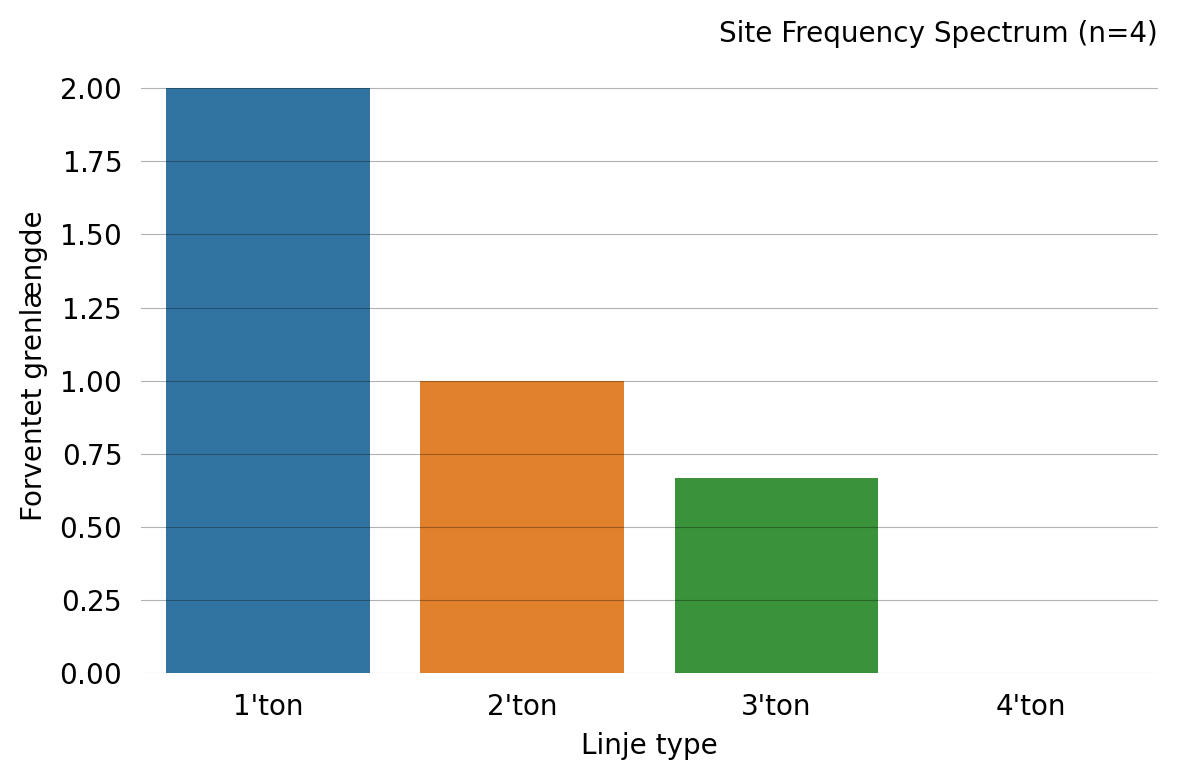
\includegraphics[width=6.13542in,height=4.0625in]{index_files/figure-latex/..-notebooks-01_coalescent_basics-fig-sfs-output-1.png}

}

\caption{\label{fig-sfs}Site Frekvens Spektrum for \(n=4\). Forventet
grenlængde per frekvensklasse beregnet via reward-transformation:
singletons (blå, \(\mathbb{E}[L_1]=2.0\)), doubletons (orange,
\(\mathbb{E}[L_2]=1.0\)) og tripletons (grøn,
\(\mathbb{E}[L_3]=0.667\)). Singletons dominerer fordi ydre grene altid
er kortere end interne grene i Kingmans coalescent.}

\end{figure}%

Singleton-dominansen ses tydeligt. Mutationer, der kun forekommer i ét
individ, er de hyppigste, mens antallet af mutationer falder hurtigt for
større frekvensklasser. SFS giver dermed et detaljeret billede af
variationen i data. Hvis man ønsker at beregne fordelinger, momenter og
kovarianser for sådanne størrelser analytisk, kræver det imidlertid et
mere generelt matematisk værktøj nemlig fase-type fordelinger.

\section{Fase-type fordelinger}\label{fase-type-fordelinger}

Coalescent-processen kan beskrives som en absorptionsproces i en
kontinuert-tid-Markov-kæde. Processen starter med et \(n\) aktive linjer
og absorberes, når alle linjer er coalesceret til MRCA. Denne type
processer beskrives naturligt ved hjælp af fase-type fordelinger (Bladt
and Nielsen 2017; Hobolth et al. 2024).

En fase-type fordeling beskriver absorptionstiden \(\tau\) i en
kontinuert-tids Markov-kæde med \(p\) transiente tilstande og én
absorberende tilstand. Systemet beskrives ved intensitetsmatricen
(Hobolth et al. 2024): \[
\Lambda = \begin{pmatrix} \mathbf{T} & \mathbf{t} \\ \mathbf{0} & 0 \end{pmatrix},
\] hvor \(\mathbf{T}\) er sub-intensitetsmatricen for de transiente
tilstande. Diagonalelementerne i \(T\) er negative og angiver den
samlede rate, hvormed processen forlader en tilstand. Vektoren
\(\mathbf{t} = -\mathbf{T}\mathbf{e}\) angiver exit-raterne fra de
transiente tilstande til den absorberende tilstand, hvor \(e\) er en
søjlevektor bestående af ettaller. Vi skriver \[
\tau \sim \mathrm{PH}(\alpha, \mathbf{T})
\] hvor \(\alpha\) angiver startfordelingen over de transiente
tilstande. Frodelen ved denne repræsentation er, at tæthedsfunktioner,
fordelinger og momenter kan beregnes direkte ved hjælp af
matrixoperationer (Bladt and Nielsen 2017): \[
f_\tau(s) = \alpha \, e^{\mathbf{T}s} \, \mathbf{t}, \qquad
\mathbb{E}[\tau] = \alpha(-\mathbf{T})^{-1}\mathbf{e}, \qquad
\mathbb{E}[\tau^n] = n!\,\alpha(-\mathbf{T})^{-n}\mathbf{e}.
\] Matricen \[
\mathbf{U} = (-\mathbf{T})^{-1}
\] kaldes Green-matricen. Det \((i,j)\)-te element i \(U\) angiver, hvor
lang tid processen i forventning tilbringer i tilstand \(j\), givet at
processen starter i tilstand \(i\). Disse forventede opholdstider kaldes
også sojourn-tider.

For Kingmans coalescent er træhøjden \(H\) fase-type fordelt med
startvektor \[
\alpha = (1, 0, \ldots, 0)
\] fordi processen starter i tilstanden med \(n\) aktive linjer.
Sub-intensitetsmatricen kan skrives som (Hobolth et al. 2024): \[
\mathbf{T} = \begin{pmatrix} -\lambda_n & \lambda_n & & \\ & -\lambda_{n-1} & \lambda_{n-1} & \\ & & \ddots & \\ & & & -\lambda_2 \end{pmatrix}, \qquad \lambda_k = \binom{k}{2}.
\] Her angiver \(\lambda_k\) den samlede rate for en
coalescent-hændelse, når der er \(k\) linjer tilstade. I \texttt{phasic}
konstrueres dette tilstandsrum automatisk ud fra en callback-funktion,
der definerer hvilke overgange der er mulige og med hvilke rater. For
\(n = 4\) er tilstandene beskrevet ved vektoren \[
(s_1, s_2, s_3, s_4)
\] hvor \(s_i\) angiver antallet af linjer, der har præcis \(i\)
efterkommere i stikprøven. Denne repræsentation gør det mulit at holde
styr på, hvilke dele af genealogien der bidrager til de forskellige
frekvensklasser i SFS. Starttilstanden er \((4,0,0,0)\) hvilket svarr
til fire separate linjer, der hver har én efterkommer i stikprøven.
Absorptionstilstanden er \((0,0,0,1)\) hvor alle fire sekvenser har
coalesceret til én fælles forfader. Dette er også illustreret i
Figur~\ref{fig-graf}.

\begin{figure}[!htbp]

\centering{

\pandocbounded{
\includegraphics[keepaspectratio]{index_files/mediabag/index_files/figure-latex/..-notebooks-01_coalescent_basics-fig-graf-output-1.pdf}}

}

\caption{\label{fig-graf}Tilstandsrum for Kingmans coalescent med
\(n=4\) prøver. Tilstandsvektoren \((s_1, s_2, s_3, s_4)\) tæller det
antal linjer der har henholdsvis \(1\), \(2\), \(3\) og \(4\)
efterkommere. Starttilstanden \((4,0,0,0)\) repræsenterer fire separate
linjer; absorptionstilstanden \((0,0,0,1)\) er MRCA. Pilene viser mulige
koalescensstransitioner med tilhørende rater.}

\end{figure}%

Fase-type repræsentationen giver adgang til langt mere end blot
træhøjden. Mange populationsgenetiske størrelser kan beskrives som
akkumulerede størrelser langs processen snarere end som absorptionstider
i sig selv. Dette leder til reward-transformationer og den multivariate
fase-type teori.

\section{Reward-transformationer og multivariat
fase-type}\label{reward-transformationer-og-multivariat-fase-type}

En af de mest nyttige egenskaber ved fase-type fordelinger er, at
teorien kan udvides til at beskrive størrelser, der akkumuleres langs en
Markov-proces. I coalescent-sammenhæng er man ofte interesseret i, hvor
lang tid processen tilbringer i bestemt typer af tilstande. Det gælder
eksempelvis den totale grenelængde, ydre grenelængde eller grenlængder
knyttet til bestemte frekvensklasser i SFS.
Figur~\ref{fig-pdf-grenlangder} viser PDF og CDF for singleton-,
doubleton- og tripleton-grenlængder beregnet ved hjælp af
reward-transformationer.

\begin{figure}[!htbp]

\centering{

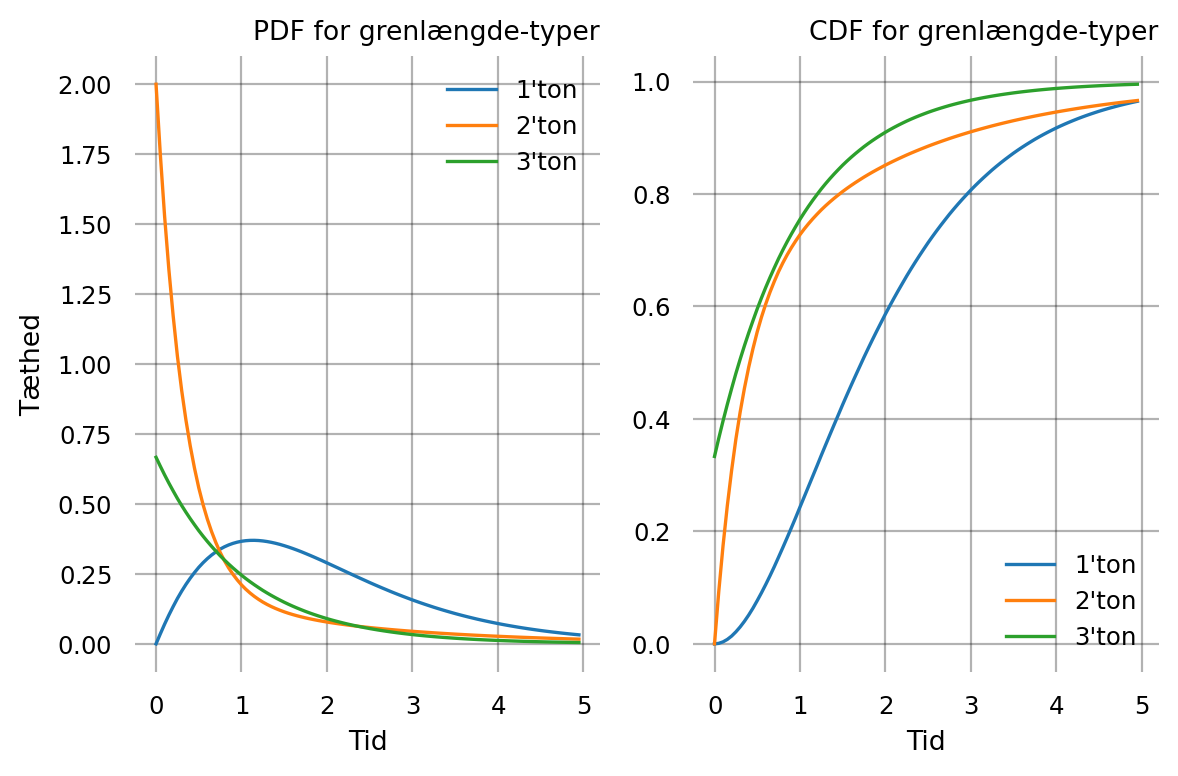
\includegraphics[width=7.17708in,height=3.02083in]{index_files/figure-latex/..-notebooks-01_coalescent_basics-fig-pdf-grenlangder-output-1.png}

}

\caption{\label{fig-pdf-grenlangder}PDF og CDF for singleton- (blå),
doubleton- (orange) og tripleton-grenlængder (\(n=4\)).
Singleton-fordelingen er en blanding af eksponentielle fordelinger og
udviser en bred tunge; tripleton-fordelingen er mere koncentreret. Den
absorberende tilstand bidrager til en spids ved \(t=0\) for tripletons.}

\end{figure}%

Ideen bag reward-transformationer er, at hver tilstand tildeles en vægt,
også kaldet en reward. Når processen bevæger sig gennem tilstandsrummet,
akkumuleres den vægtede tid. Hvis \(r(i)\) angiver reward-værdien i
tilstand \(i\), kan den samlede reward skrives som \[
\tilde{\tau} = \int_0^\tau r(X_t),dt.
\] Et centralt resultat i fase-type teorien er, at denne størrelse igen
er fase-type fordelt, når alle rewards er positive (Bladt and Nielsen
2017). Mere præcist gælder \[
\tilde{\tau} \sim \mathrm{PH}\!\bigl(\alpha,\, \Delta(\mathbf{r})^{-1}\mathbf{T}\bigr).
\] Hvor \(\delta(r)\) er diagonalmatrixen med reward-værdierne på
diagonalen. Hvis nogle rewards er nul, kræver repræsentationen en særlig
håndtering, da der kan opstå en sandsynlighedsmasse ved nul.

Den totale grenelængde \(L\) er et vigtigt eksempel på en
reward-transformeret størrelse. Når der er \(k\) aktive linjer i
genealogien, bidrager hver linje med til den akkumulerede tid.
Reward-vektoren bliver derfor \[
\mathbf{r}_L=(n,n-1,\ldots,2).
\] Den totale grenelængde kan dermed fortolkes som en version af
træhøjden \(H\). På samme måde kan man konstruere rewards, der kun
tæller bestemte typer grene, eksempelvis ydre grene eller grene med et
bestemt antal efterkommere.

I praksis er man ofte interesseret i flere størrelser på samme tid.
Træhøjde, total grenelængde og ydre grenelængde beskriver forskellige
aspekter af den samme genealogi og er derfor statistisk afhængige. For
at håndtere dette udvides teorien til multivariate fase-type fordelinger
(MPH).

I MPH kobles flere reward-vektorer til den samme underliggende
Markov-proces. Det gør det muligt at beregne fælles fordelinger,
kovarianser og blande momenter analytisk. For to reward-transformerede
variable \(Y_1\) og \(Y_2\) er det blandede moment givet ved (Hobolth et
al. 2024) \[
\mathbb{E}[Y_1 Y_2] = \alpha \mathbf{U} \Delta(\mathbf{r}_1) \mathbf{U} \Delta(\mathbf{r}_2) \mathbf{e} + \alpha \mathbf{U} \Delta(\mathbf{r}_2) \mathbf{U} \Delta(\mathbf{r}_1) \mathbf{e},
\] Hvor \(U=(-T)^-1\) er Green-matricen

For et lille eksempel med \(n=3\) sekvenser kan man beskrive træhøjde,
total grenelængde, ydre grenelængde og indre grenelængde simultant som
\[
(H, L, E, I) \sim \mathrm{MPH}\!\left(\mathbf{e}_1, \mathbf{T}, \mathbf{R}\right), \qquad
\mathbf{T} = \begin{pmatrix} -3 & 3 \\ 0 & -1 \end{pmatrix}, \quad
\mathbf{R} = \begin{pmatrix} 1 & 3 & 3 & 0 \\ 1 & 2 & 1 & 1 \end{pmatrix}.
\] Her beskriver \(T\) den underliggende coalescent-proces, mens \(R\)
angiver de rewards, der bruges til at beregne de fire størrelser
(Hobolth et al. 2024). På den måde kan forventninger, varianser og
kovarianser udledes analytisk uden at simulere genealogier.

Indtil nu har fokus været på kontinuerte størrelser som tider og
grenlængder. Mange af de størrelser, der observeres direkte i genetiske
data, er imidlertid diskrete. Det gælder for eksempel antallet af
segregerende sites og de enkelte komponenter i SFS. For at beskrive
sådanne størrelser udvides teorien derfor til diskrete
fase-type-fordelinger.

\section{Den diskrete fase-type fordeling og segregerende
sites}\label{den-diskrete-fase-type-fordeling-og-segregerende-sites}

Mens fase-type fordelinger beskriver kontinuerte variable, såsom tider
og grenelængder, beskriver diskrete fase-type fordelinger (DPH)
tællevariable. Det gør dem særligt velegnede til at modellere
mutationsdata, hvor man for eksempel er interesseret i antallet af
segregerende sites. En måde at forstå konstruktionen på er at betragte
forholdet mellem mutationer og coalescent-hændelser som en konkurrence.
Når processen befinder sig i en tilstand med \(k\) aktive linjer, kan
den næste hændelse enten være en mutation eller en coalescenthændelse.
Sandsynligheden for at næste hændelse er en mutation er (Hobolth et al.
2021): \[
p_k = \frac{\theta/2}{\theta/2 + \binom{k}{2}} = \frac{\theta}{\theta + k(k-1)}.
\] Denne konkurrence mellem mutation og coalescent giver anledning til
en diskret Markov-kæde, som kan analyseres ved hjælp af DPH-teorien. Et
vigtigt resultat er, at antallet af segregerende sites kan beskrives
direkte ved en diskret fase-type fordeling. Betinget på den
underliggende genealogi gælder (Hobolth et al. 2024) \[
S+1 \sim \mathrm{DPH} (\alpha_L,\mathbf P),
\] Hvor \[
{P} = \left(\mathbf{I} - \frac{2}{\theta}\mathbf{T}_L\right)^{-1}.
\] Denne repræsentation gør det muligt at beregne sandsynligheder og
likelihoods analytisk i stedet for udelukkende at basere sig på
simulation. På samme måde kan de enkelte komponenter i SFS beskrives ved
diskrete fase-type fordelinger. Dermed kan man ikke blot beregne
forventninger, men hele fordelinger samt kovarianser mellem forskellige
frekvensklasser.

Indtil videre modellerne taget udgangspunkt i et enkelt locus. I
virkelige genomer er situationen imidlertid mere kompleks, fordi
rekombination betyder, at forskellige positioner i genomet kan have
forskellige genealogier.

Standard-coalescenten antager, at alle positioner i et kort locus kan
approksimeres som om, de deler den samme genealogi. Dette er en rimelig
approksimation for korte DNA-segmenter, men bliver mindre realistisk,
når man analyserer større dele af genomet (Wakeley 2009). Årsagen er
rekombination. Under meiosen kan genetisk materiale udveksles mellem
kromosomer, hvilket betyder, at forskellige dele af genomet kan nedarves
fra forskellige forfædre. To nærliggende positioner i genomet vil derfor
ikke nødvendigvis have den samme genealogi. For at beskrive dette
udvides coalescent til et ancestral recombination graph (ARG). Hvor den
klassiske coalescent-proces kun indeholder hændelser, hvor linjer
samles, indeholder ARG'et både coalescent- og rekombinationshændelser.
De to typer hændelser har modsatrettede effekter. Coalescent-hændelser
reducerer antallet af aktive linjer ved at samle dem, mens rekombination
kan splitte ancestrale linjer op og skabe nye genealogiske forbindelser.
Resultatet er et mere komplekst tilstandsrum. Dette er illustreret
Figur~\ref{fig-arg-graph}, som viser tilstandsrummet for to-locus
ARG-modellen med \(n=2\).

\begin{figure}[!htbp]

\centering{

\pandocbounded{
\includegraphics[keepaspectratio]{index_files/mediabag/index_files/figure-latex/..-notebooks-05_joint_probability_inferens-fig-arg-graph-output-1.pdf}}

}

\caption{\label{fig-arg-graph}Tilstandsrum for to-locus ARG-modellen med
\(n=3\) prøver. Tilstandsvektoren tracker lineager med afstamninger fra
locus 1, locus 2 eller begge. Pile viser koalescentovergange og
rekombinationsovergange, og absorptionstilstanden nås når alle lineager
enten er coalesceret eller skilt ad ved rekombination.}

\end{figure}%

Sammenlignet med standard coalescent (Figur~\ref{fig-graf}) er antallet
af mulige tilstande væsentligt større, selv for små stikprøvestørrelser.
Dette skyldes, at modellen nu skal holde styr på, hvilke dele af genomet
der deler fælles historie, og hvilke der allerede er blevet adskilt af
rekombination.

Rekombination parameteren \[
\rho = 4N_e r
\] beskriver styrken af rekombinationsprocessen på samme måde, som \[
\theta = 4N_e \mu
\] beskriver mutationsprocessen. ARG-modeller giver mulighed for at
udnytte information fra hele genomer frem for et enkelt loci. Samtidig
illustrerer de, hvordan fase-type teorien kan anvendes på langt mere
komplekse genealogiske strukturer end den klassiske standard coalescent.

En anden vigtig generalisering af standard coalescent er at tage højde
for populationsstruktur. I naturen er populationer sjældent fuldstændigt
homogene og migration mellem geografisk adskilte populationer kan have
stor betydning for de genealogiske mønstre, der observeres i data.

\section{Populationsstruktur: to-ø-modellen og
IM-modellen}\label{populationsstruktur-to-uxf8-modellen-og-im-modellen}

Den klassiske standard coalescent bygger på antagelsen om panmixi, dvs.
at alle individer i populationen har samme sandsynlighed for at
reproducere med hinanden. Denne antagelse er sjældent fuldt realistisk.
Geografiske barrierer, habitatfragmentering og begrænset spredning
betyder ofte, at individer primært udveksler gener med nærliggende
populationer.

Når populationer er opdelt i delpopulationer, ændres genealogierne
markant. To individer fra samme delpopulation vil typisk dele en fælles
forfader hurtigere end to individer fra forskellige delpopulationer.
Genealogien indeholder derfor information ikke kun om
populationsstørrelse, men også om migration mellem populationer.

En af de simpleste modeller for populationsstruktur er to-ø-modellen.
Modellen består af to populationer, hvor der foregår migration mellem
populationerne med en konstant migrationsrate \(m\). Inden for hver
population følger processen de samme grundprincipper som
standard-coalescenten, men der tilføjes migrationsovergange mellem
populationerne (Hobolth et al. 2024).

Hvis to linjer befinder sig i samme population, kan de coalescere
direkte. Hvis de derimod befinder sig i forskellige populationer, må
mindst én af linjerne først migrere, før en coalescent-hændelse kan
finde sted. Migration påvirker derfor den genealogiske proces ved at
ændre, hvilke linjer der kan coalescere med hinanden.

For at beskrive dette må tilstandsrummet udvides. Hver linje
karakteriseres nu ikke alene ved antallet af efterkommere i stikprøven,
men også ved hvilken population linjen aktuelt befinder sig i. Dette
giver en mere kompleks Markov-kæde end den klassiske standard
coalescent.

\begin{figure}[!htbp]

\centering{

\pandocbounded{
\includegraphics[keepaspectratio]{index_files/mediabag/index_files/figure-latex/..-notebooks-03_svgd_two_island-fig-two-island-graph-output-1.pdf}}

}

\caption{\label{fig-two-island-graph}Tilstandsrum for to-ø modellen med
\(n=2\) linjer. Tilstandsvektoren \((s_1, s_2, \text{pop})\) tracker om
de to linjer befinder sig i population \(1\), population \(2\) eller er
delt. Pile angiver mulige overgange: koalescentovergange (blå) sker
inden for samme population; migrationsovergange (rød) sender en linje
fra én population til den anden. Absorptionstilstanden MRCA nås når
begge linjer er i samme population og koalescerer.}

\end{figure}%

Figur~\ref{fig-two-island-graph} illustrerer, hvordan migration og
coalescent konkurrerer med hinanden. Coalescenthændelser reducerer
antallet af aktive linjer, mens migration flytter linjer mellem
populationerne. Selv med blot to linjer bliver tilstandsrummet
betydeligt større end i standard coalescent (Figur~\ref{fig-graf}).

I denne model parametriseres processerne ved \[
\theta_0 = 4N_e\mu
\] og \[
\theta_1 = 4N_em,
\] hvor \(\mu\) er mutationsraten og \(m\) migrationsraten.

En vigtig statistisk udfordring ved modellen er identificerbarhed. Høj
migration og høj coalescentrate kan producere meget lignende
genealogiske mønstre. Begge mekanismer fører til korte TMRCA-tider og
dermed relativt ens fordelinger af genetisk variation. Når migrationen
bliver meget høj, bliver det derfor vanskeligt at afgøre, om et
observeret mønster skyldes hyppig migration eller hurtig coalescent.

Selvom to-ø-modellen er et vigtigt skridt mod mere realistiske modeller,
beskriver den stadig populationerne som stationære gennem hele deres
historie. I mange biologiske situationer er man imidlertid interesseret
i populationer, der på et bestemt tidspunkt har splittet sig fra en
fælles ancestral population. Dete beskrives ved
isolation-with-migration-modellen (IM-modellen).

IM-modellen kombinerer populationsstruktur med et historisk
split-tidspunkt. Modellen antager, at de to nuværende populationer
opstod fra en fælles ancestral population for \(t_s\) generationer
siden. Fra nutiden og tilbage til split-tidspunktet udvikler
populationerne sig som en struktureret model med migration. Før
split-tidspunktet eksisterer der kun én fælles ancestral population.

De Nutidige populationer kan være delvist adskilte, men de deler stadig
en fælles evolutionær fortid. Et vigtigt aspekt ved IM-modellen er, at
den er tidsinhomogen. Overgangsraterne ændrer sig ved split-tidspunktet
og processen kan derfor ikke beskrives af én enkelt generator-matrix for
hele tidsforløbet. I stedet opdeles historien i epoker med forskellige
rater.

Denne tilgang gør det muligt at beskrive hændelser såsom
populationssplit, flaskehalse og ekspansioner, som kan efterlade
karakteristiske signaler i TMRCA-fordelingen og i SFS
(Figur~\ref{fig-sfs-epoch}).

\begin{figure}[!htbp]

\centering{

\pandocbounded{
\includegraphics[keepaspectratio]{index_files/mediabag/index_files/figure-latex/..-notebooks-04_time_inhomogeneous-fig-sfs-epoch-output-1.pdf}}

}

\caption{\label{fig-sfs-epoch}SFS under \(3\)-epoke model med \(n=10\)
og population-størrelser \(N_e=[1, 5, 10]\) (nuværende, fortid, fjern
fortid). Blå søjler: singletons (\(1\)-ton); orange: doubletons
(\(2\)-ton); grøn: tripletons (\(3\)-ton); osv. Singletons dominerer
kraftigt (\(>40\%\) af total grenlængde) fordi den nuværende lille
population (\(N_e=1\)) giver mange korte ydre grene som producerer
singletons. Fortidens store population (\(N_e=10\)) bidrager med lange
interne grene der giver flatere højere frekvenser.}

\end{figure}%

I sådanne modeller afhænger formen af SFS både af
populationsstørrelserne i de enkelte epoker og af epokerenes varighed.
Et overskud af sjældne varianter, for eksempel singletons, forbindes
ofte med nylig populationsvækst, mens flaskehalse og populationsstruktur
kan ændre spektret på mere komplekse måder. Derfor skal SFS fortolkes i
sammenhæng med den konkrete model. I \texttt{phasic} kan tidsinhomogene
modeller håndteres ved at opbygge processen epoke for epoke og kombinere
dem analytisk. Det gør det muligt at beregne fordelinger og momenter for
relativt komplekse demografiske modeller uden at skulle basere analysen
på omfattende simulationer (Røikjer et al. 2022; Munch 2026).

\section{Bayesiansk inferens med
SVGD}\label{bayesiansk-inferens-med-svgd}

I dette speciale anvendes Bayesiansk inferens. Her beskrives
posteriorfordelingen som \[
\pi(\theta \mid \mathbf{x}) \propto p(\mathbf{x} \mid \theta)\, \pi_0(\theta).
\] Her repræsenterer \(p(\mathbf x\mid\theta)\) likelihooden, mens
\(\pi_0(\theta)\) er priorfordelingen.

En fordel ved Bayesiansk inferens er, at usikkerheden omkring
parameteren kvantificeres direkte. I stedet for kun at givet ét
punktestimat opnår man en hel sandsynlighedsfordeling over mulige
parameterværdier. Dette er relevant, hvor data ofte er støjfyldte og
hvor flere forskellige parameterkombinationer kan forklare de samme
observationsmønstre.

En central udfordringen er dog, er at posteriorfordelingen sjældent kan
beregnes analytisk. For komplekse coalescentmodeller bliver integralerne
hurtigt uoverskuelige og man må derfor benytte numeriske metoder. Den
klassiske tilgang er er Markov Chain Monte Carlo (MCMC), men sådanne
metoder kan være beregningstunge og langsomme for de grafbaserede
modeller, der anvendes i dette speciale.

Derfor benyttes Stein Variational Gradient Descent (SVGD) (Liu and Wang
2016). SVGD repræsenterer posterioren ved en samling partikler \[
{\theta_1,\theta_2,\ldots,\theta_{n_p}}
\] som iterativt flyttes gennem parameterrummet. Opdateringen af hver
partikel er givet ved \[
\theta_i \leftarrow \theta_i + \epsilon\, \hat{\phi}^*(\theta_i)
\] Hvor \[
\hat{\phi}^*(\theta) = \frac{1}{n_p}\sum_{j=1}^{n_p}\Bigl[k(\theta_j, \theta)\,\nabla_{\theta_j}\log\pi(\theta_j\mid\mathbf{x}) + \nabla_{\theta_j}k(\theta_j, \theta)\Bigr],
\] De to led i opdateringen har forskellige funktioner. Det første led
trækker partiklerne mod områder med høj posterior sandsynlighed. Det
andet led virker frastødende og forhindrer partiklerne i at kollapse til
et enkelt punkt. Kombinationen af de to mekanismer gør det muligt at
approksimere hele posteriorfordelingen frem for blot dens maksimum (Liu
and Wang 2016).

\section{Bavianer som modelsystem}\label{bavianer-som-modelsystem}

Modellerne i notebooks 01--06 testes udelukkende på simulerede data med
kendte sande parametre. Formålet er til sidst at anvende dem på rigtige
biologiske data og til det bruges bavianer slægten \emph{Papio} som
modelsystem.

\emph{Papio} er en gruppe af nært beslægtede primater, som lever i store
dele af Afrika (Kopp et al. 2023). Slægten består af seks nulevende
arter:

\begin{itemize}
\tightlist
\item
  Olive bavian (\emph{Papio anubis}),
\item
  Yellow bavian (\emph{Papio cynocephalus}),
\item
  Chacma bavian (\emph{Papio ursinus}),
\item
  Guinea bavian (\emph{Papio papio}),
\item
  Hamadryas bavain (\emph{Papio hamadryas})
\item
  Kinda bavain (\emph{Papio kindae}).
\end{itemize}

Disse seks arter adskilles i to klader: en nordlig klade bestående af
\emph{P. hamadryas}, \emph{P. anubis} og \emph{P. papio} og en sydlig
klade bestående af \emph{P. kindae}, \emph{P. cynocephalus} og \emph{P.
ursinus} som divergerede fra en fælles stamfader for mere end 1 million
år siden ({Rogers et al.} 2019; {Vilgalys et al.} 2022). Den geografiske
fordeling og hybridzonerne er vist i Figur~\ref{fig-Kort}.

\begin{figure}[!htbp]

\centering{

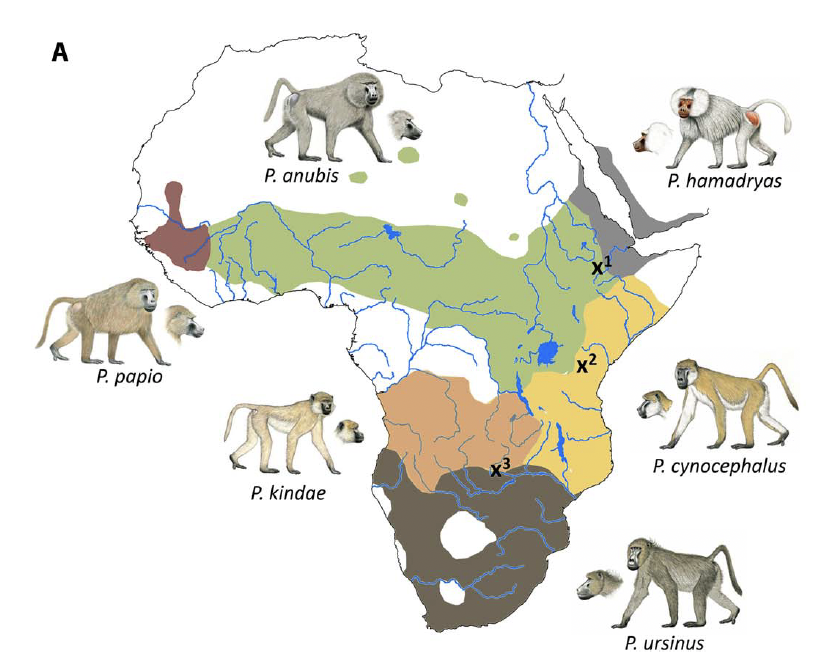
\includegraphics[width=0.5\linewidth,height=\textheight,keepaspectratio]{illustrations/Kort.png}

}

\caption{\label{fig-Kort}\emph{Papio} baboon arter. Nuværende udbredelse
af hver bavianart samt placeringen af tre veldokumenterede aktive
hybridzoner er også vist. x1: hybridzone mellem \emph{P. hamadryas} og
\emph{P. anubis}, x2: hybridzone mellem \emph{P. cynocephalus} og
\emph{P. anubis}, x3: hybridzone mellem \emph{P. kindae} og \emph{P.
ursinus}. Billede fra {Rogers et al.} (2019).}

\end{figure}%

På trods af disse geografiske adskillelser kan flere arter krydse sig
med hinanden i naturen og producere fertile hybrider ({Sørensen et al.}
2023; {Jordan et al.} 2018). I flere kontaktzoner er der
veldokumenterede hybridzoner med løbende genflow. {Rogers et al.} (2019)
analyserede helgenomsekvenseringsdata for alle seks arter og
dokumenterede multiple episoder af admixture og introgression, herunder
genetisk bidrag fra en uidentificeret ancestral linje til \emph{P.
papio} og aktiv nuklear DNA-swamping ved hybridzonen mellem \emph{P.
anubis} og \emph{P. cynocephalus}.

Som det fremgår af Figur~\ref{fig-Kort}, overlapper arterne geografisk
ved en række hybridzoner, hvor aktiv genudveksling er dokumenteret
({Sørensen et al.} 2023). {Sørensen et al.} (2023) udvidede denne
analyse til 225 vilde bavianer fra 19 lokaliteter og dokumenterede
admixture mellem \emph{P. anubis} og \emph{P. cynocephalus} i det
sydlige Tanzania, en tæt genealogisk forbindelse mellem Kinda-bavianer
og yellow-bavianerne, samt tegn på tre-vejs admixture i
yellow-bavianeren, et mønster som ikke tidligere er observeret i denne
slægt.

Bavianernes evolutionære historie begyndte omtrent samtidig med
evolutionen af menneskeslægten \emph{Homo}, altså for omkring 2
millioner år siden ({Rogers et al.} 2019). I modsætning til mennesker,
hvor kun en art eksisterer i dag, har bavianer bevaret flere linjer.
PSMC-analyser (Li and Durbin 2011) viser, at alle seks populationer har
oplevet fald i effektiv populationsstørrelse de seneste 100.000 år,
sandsynligvis i forbindelse med klimatiske ændringer ({Rogers et al.}
2019). Det gør dem særligt velegnede som modelsystem til at studere både
divergens og hybridisering i naturlige populationer.

\section{Data}\label{data}

I dette speciale anvendes data fra {Sørensen et al.} (2023), som udførte
helgenomsekventering af \(225\) vilde bavianer fra 19 lokaliteter
fordelt over Afrika. Kromosom \(20\) indeholder i dette datasæt
\(2.665.269\) varianter fordelt over \(227\) diploide individer svarende
til \(454\) haploide kromosomer.

Her bruges data fra seks arter med følgende antal segregerende SNPs og
haploide prøver:

\begin{itemize}
\tightlist
\item
  \emph{P. cynocephalus} \(1.379.280\) SNPs (\(n=120\)),
\item
  \emph{P. anubis} \(1.058.781\) SNPs (\(n=180\)),
\item
  \emph{P. kindae} \(833.071\) SNPs (\(n=50\)),\\
\item
  \emph{P. hamadryas} \(460.025\) SNPs (\(n=48\)),
\item
  \emph{P. ursinus} \(403.120\) SNPs (\(n=8\)),
\item
  \emph{P. papio} \(110.086\) SNPs (\(n=24\)).
\end{itemize}

Den mindste population i datasættet er \emph{P. ursinus}, som kun har
\(8\) haploide prøver. Dette sætter den øvre grænse for dirkete
sammenligninger af SFS på tværs af arter.

For hvert individ er der beregnet allelfrekvenser per position i
genomet. Disse angiver antallet af afledte alleler ud af det samlede
antal sekvenser ved et givent site. Allele counts anvendes som input til
inferensmodellerne. Mutationsdiversiteten estimeres blandt andet ved.
hjælp af Wattersons estimator, \[
\hat{\theta}_W = \frac{S}{a_n}
\] Hvor \(S\) er antallet af segregerende sites, og \(a_n\) er det
harmoniske tal.

Mutationsraten, \(\mu = 0{,}9 \times 10^{-8}\) angivet som mutationer
per basepar per generation, samt generationstiden \(g = 11\) år, er
hentet fra {Sørensen et al.} (2023). Disse værdier bruges til at omregne
skalerede modelparametre til biologisk størrelse der kan tolkes, såsom
effektiv populationsstørrelse (\(N_e\)) og tid angivet i år.

\section{Modeller og implementering}\label{modeller-og-implementering}

Alle coalescentmodeller er implementeret i \texttt{phasic} (Munch 2026)
og er valideret både analytisk og ved sammenligning med simulationer
udført i msprime.

I alle analyser anvendes \(n_{\text{samples}} = 8\) haploide prøver til
enkeltpopulationsmodellen, bestemt via systematisk test i NB02. Til to-ø
modellen og IM-modellen bestemmes \(n_{\text{samples}}\) per population
via test i NB03. Tilstandsrummets størrelse vokser eksponentielt med
\(n_{\text{samples}}\) og valget er et kompromis mellem statistisk
præcision og beregningseffektivitet.

Analysen er bygget op omkring syv Jupyter notebooks. De syv notebooks er
organiseret så hver bygger videre på den foregående, fra grundlæggende
verificering til anvendelse på rigtige bavian-data. Oversigten er vist i
Tabel~\ref{tbl-notebooks}.

\begin{longtable}[]{@{}
  >{\raggedright\arraybackslash}p{(\linewidth - 6\tabcolsep) * \real{0.2500}}
  >{\raggedright\arraybackslash}p{(\linewidth - 6\tabcolsep) * \real{0.2500}}
  >{\raggedright\arraybackslash}p{(\linewidth - 6\tabcolsep) * \real{0.2500}}
  >{\raggedright\arraybackslash}p{(\linewidth - 6\tabcolsep) * \real{0.2500}}@{}}
\caption{Oversigt over notebooks og modeller implementeret i dette
speciale.}\label{tbl-notebooks}\tabularnewline
\toprule\noalign{}
\begin{minipage}[b]{\linewidth}\raggedright
Notebook
\end{minipage} & \begin{minipage}[b]{\linewidth}\raggedright
Model
\end{minipage} & \begin{minipage}[b]{\linewidth}\raggedright
Parametre
\end{minipage} & \begin{minipage}[b]{\linewidth}\raggedright
Formål
\end{minipage} \\
\midrule\noalign{}
\endfirsthead
\toprule\noalign{}
\begin{minipage}[b]{\linewidth}\raggedright
Notebook
\end{minipage} & \begin{minipage}[b]{\linewidth}\raggedright
Model
\end{minipage} & \begin{minipage}[b]{\linewidth}\raggedright
Parametre
\end{minipage} & \begin{minipage}[b]{\linewidth}\raggedright
Formål
\end{minipage} \\
\midrule\noalign{}
\endhead
\bottomrule\noalign{}
\endlastfoot
NB01 & Kingmans coalescent & \(\theta\) & Verificering af fase-type
implementering og analytiske egenskaber \\
NB02 & SVGD-kalibrering & Læringsrate, prior, \(n_{\text{obs}}\),
\(n_{\text{samples}}\), partikler & Systematisk valg af
inferenskonfiguration til bavian-analyser \\
NB03 & To-ø modellen & \(\theta_0\), \(\theta_1\) & Identificerbarhed og
sammenligning med method of moments \\
NB04 & Tidsinhomogen coalescent og IM-modellen & \(\theta_0\),
\(\theta_1\), \(t_s\) & Flaskehalse, ekspansioner og
split-tidspunkter \\
NB05 & Joint probability-inferens & \(\theta\), \(\mu\),
\texttt{reward\_limit} & Diskrete SFS-observationer og sammenligning med
TMRCA-inferens \\
NB06A & Enkeltpopulationsanalyse & \(\theta\), \(N_e\) & SVGD-inferens
på bavian-data for seks \emph{Papio}-arter \\
NB06B & To-populations analyse & \(\theta_0\), \(\theta_1\), \(t_s\) &
Migration og split-tidspunkter for bavian-artpar \\
\end{longtable}

\chapter{Resultater}\label{resultater}

Resultatafsnittet følger analysens opbygning. Først verificeres
fase-type-implementeringen af Kingmans coalescent ved sammenligning med
kendte analytiske resultater. Dernæst undersøges SVGD-inferensens
stabilitet og kalibrering. Herefter analyseres to-ø-modellen,
tidsinhomogene modeller og joint probability-inferens. Til sidst
anvendes de validerede metoder på helgenomdata fra seks
\emph{Papio}-arter.

\section{Verificering af Kingmans
coalescent}\label{verificering-af-kingmans-coalescent}

Det første skridt er at kontrollere at \texttt{phasic} faktisk beregner
det rigtige. Hvis implementeringen er forkert, giver alle efterfølgende
analyser et forkert billede. Verificeringen sker ved at sammenligne
numeriske resultater fra \texttt{phasic} med kendte analytiske formler
for Kingmans coalescent.

Tabel~\ref{tbl-verificering} viser den forventede træhøjde
\(\mathbb{E}[H]\) fra \texttt{phasic} sammenlignet med den analytiske
formel \(\sum_{k=2}^n \frac{2}{k(k-1)}\) for \(n=2\) til \(n=8\).
Forskellen er nul for alle prøvestørrelser, og implementeringen er altså
korrekt.

{

\begin{longtable}[]{@{}llll@{}}

\caption{\label{tbl-verificering}Verificering af \(\mathbb{E}[H]\) mod
analytisk formel \(\sum_{k=2}^{n} 2/[k(k-1)]\) for \(n=2\) til \(n=8\).
Forskellen er nul for alle \(n\), hvilket bekræfter at phasic beregner
de korrekte forventede koalescenttider.}

\tabularnewline

\toprule\noalign{}
& E{[}H{]} numerisk & E{[}H{]} analytisk & Forskel \\
n & & & \\
\midrule\noalign{}
\endhead
\bottomrule\noalign{}
\endlastfoot
2 & 1.00000 & 1.00000 & 0.0 \\
3 & 1.33333 & 1.33333 & 0.0 \\
4 & 1.50000 & 1.50000 & 0.0 \\
5 & 1.60000 & 1.60000 & 0.0 \\
6 & 1.66667 & 1.66667 & 0.0 \\
7 & 1.71429 & 1.71429 & 0.0 \\
8 & 1.75000 & 1.75000 & 0.0 \\

\end{longtable}

}

Sojourn-times fra Tabel~\ref{tbl-sojourn} fortæller noget om, hvor
processen tilbringer sin tid. For \(n=4\) bruges kun \(0{,}167\)
coalescent-enheder med fire aktive linjer og \(0{,}333\) med tre, mens
hele \(1{,}000\) enhed bruges på den fase hvor kun to linjer er tilbage.
Den sidste fase dominerer altså den samlede TMRCA, og det er et mønster
der genfinder sig i alle størrelser af \(n\).

{

\begin{longtable}[]{@{}llll@{}}

\caption{\label{tbl-sojourn}Forventede sojourn-tider per fase for
\(n=4\). Med \(k\) aktive linjer er den forventede opholdstid
\(\mathbb{E}[T_k] = 2/[k(k-1)]\) coalescent-enheder. Fasen med \(k=2\)
linjer (\(\mathbb{E}[T_2]=1.0\)) udgør den absolut største andel af den
samlede forventede TMRCA på 1.5 coalescent-enheder.}

\tabularnewline

\toprule\noalign{}
& k linjer & Tilstande & E{[}Tₖ{]} = 2/k(k-1) \\
\midrule\noalign{}
\endhead
\bottomrule\noalign{}
\endlastfoot
0 & 4 & (4, 0, 0, 0) & 0.16667 \\
1 & 3 & (2, 1, 0, 0) & 0.33333 \\
2 & 2 & (0, 2, 0, 0), (1, 0, 1, 0) & 1.00000 \\

\end{longtable}

}

Reward-transformationerne giver den forventede grenlængde per
frekvensklasse. For \(n=4\) er singleton-grenlængden \(2{,}000\),
doubleton \(1{,}000\) og tripleton \(0{,}667\) coalescent-enheder, og
den samlede grenlængde er \(\mathbb{E}[L] = 3{,}667\). Det stemmer
præcist overens med \(2 \cdot a_n = 3{,}667\), som bekræfter Wattersons
estimator. Figur~\ref{fig-sfs} viser det forventede SFS for \(n=4\).
Singletons udgør klart den største frekvensklasse, fordi ydre grene er
kortere end indre grene og de fleste mutationer derfor lander som
singletons.

\begin{figure}[!htbp]

\centering{

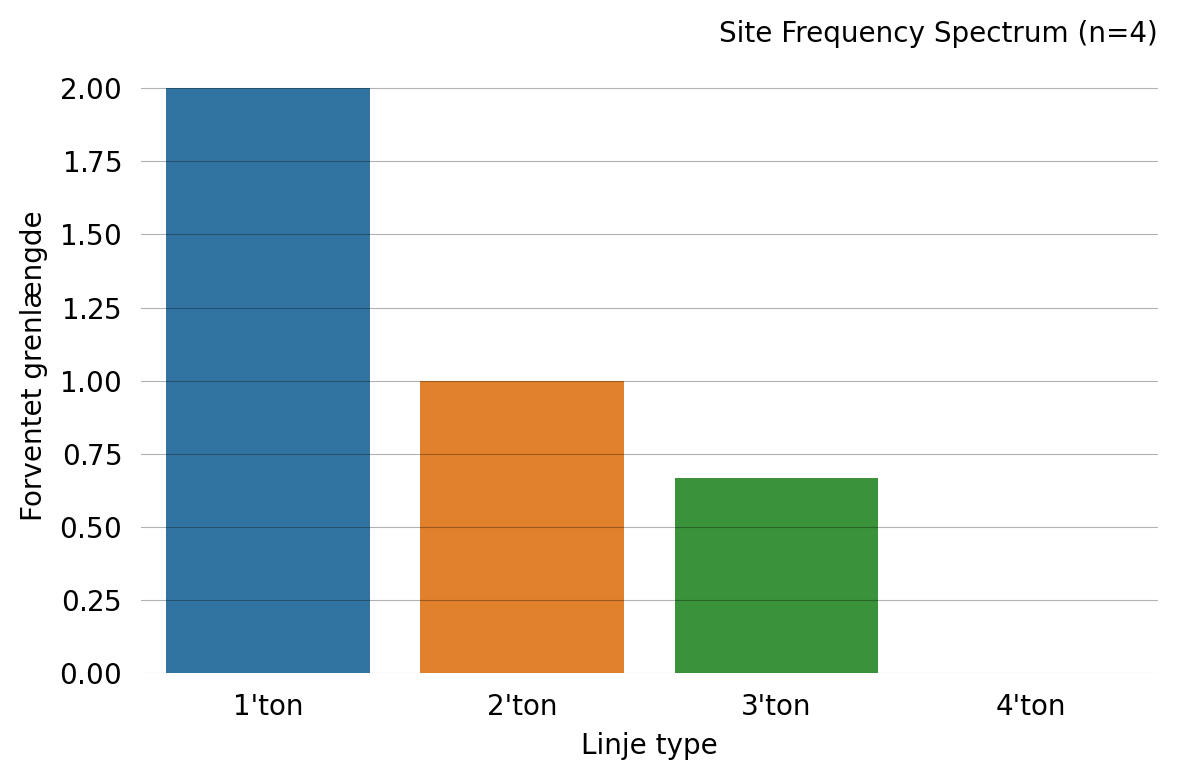
\includegraphics[width=6.13542in,height=4.0625in]{index_files/figure-latex/..-notebooks-01_coalescent_basics-fig-sfs-output-1.png}

}

\caption{\label{fig-sfs}Site Frekvens Spektrum for \(n=4\). Forventet
grenlængde per frekvensklasse beregnet via reward-transformation:
singletons (blå, \(\mathbb{E}[L_1]=2.0\)), doubletons (orange,
\(\mathbb{E}[L_2]=1.0\)) og tripletons (grøn,
\(\mathbb{E}[L_3]=0.667\)). Singletons dominerer fordi ydre grene altid
er kortere end interne grene i Kingmans coalescent.}

\end{figure}%

Det er dog ikke nok at kende forventningerne man skal også forstå,
hvordan usikkerheden ser ud. Tabel~\ref{tbl-kovarians} viser
kovariansmatricen for SFS-grenlængderne. Singleton- og
doubleton-grenlængderne er negativt korrelerede
(\(\text{Cov}(B_1, B_2) = -0{,}222\)), mens singleton og tripleton er
positivt korrelerede (\(\text{Cov}(B_1, B_3) = 0{,}889\)). Det betyder
at en naiv antagelse om uafhængighed mellem frekvensklasserne vil
undervurdere den samlede usikkerhed i inferens.

{

\begin{longtable}[]{@{}lllll@{}}

\caption{\label{tbl-kovarians}Kovariansmatrix for SFS-grenlængder
(\(n=4\)). Singletons (1-ton) og doubletons (2-ton) er negativt
korrelerede (\(\text{Cov}=-0.222\)). Singletons og tripletons er
positivt korrelerede (\(\text{Cov}=0.889\)). Diagonal-elementerne er
varianserne: \(\text{Var}[L_1]=1.778\), \(\text{Var}[L_2]=2.333\),
\(\text{Var}[L_3]=0.889\). Naiv uafhængighedsantagelse undervurderer
usikkerheden i inference.}

\tabularnewline

\toprule\noalign{}
& 1\textquotesingle ton & 2\textquotesingle ton & 3\textquotesingle ton
& 4\textquotesingle ton \\
\midrule\noalign{}
\endhead
\bottomrule\noalign{}
\endlastfoot
1\textquotesingle ton & 1.7778 & -0.2222 & 0.8889 & 0.0 \\
2\textquotesingle ton & -0.2222 & 2.3333 & -0.4444 & 0.0 \\
3\textquotesingle ton & 0.8889 & -0.4444 & 0.8889 & 0.0 \\
4\textquotesingle ton & 0.0000 & 0.0000 & 0.0000 & 0.0 \\

\end{longtable}

}

Til sidst sammenlignes \texttt{phasic} direkte med msprime på \(3000\)
simulerede genealogier. Figur~\ref{fig-msprime-validering} viser venstre
panel histogrammet over simulerede TMRCA-tider (blå) mod den analytiske
PDF (orange), og højre panel viser det simulerede SFS normaliseret som
andel af total grenlængde sammenlignet med den analytiske forventning.
De to kurver følger hinanden tæt trods at de er beregnet på helt
forskellige måder. Det simulerede \(\mathbb{E}[H] = 1{,}499\) afviger
kun \(0{,}07\%\) fra det analytiske \(1{,}500\), og den samlede relative
afvigelse er \(1{,}66\%\), som er inden for hvad man forventer ved
\(3000\) simuleringer. Implementeringen er korrekt.

\begin{figure}[!htbp]

\centering{

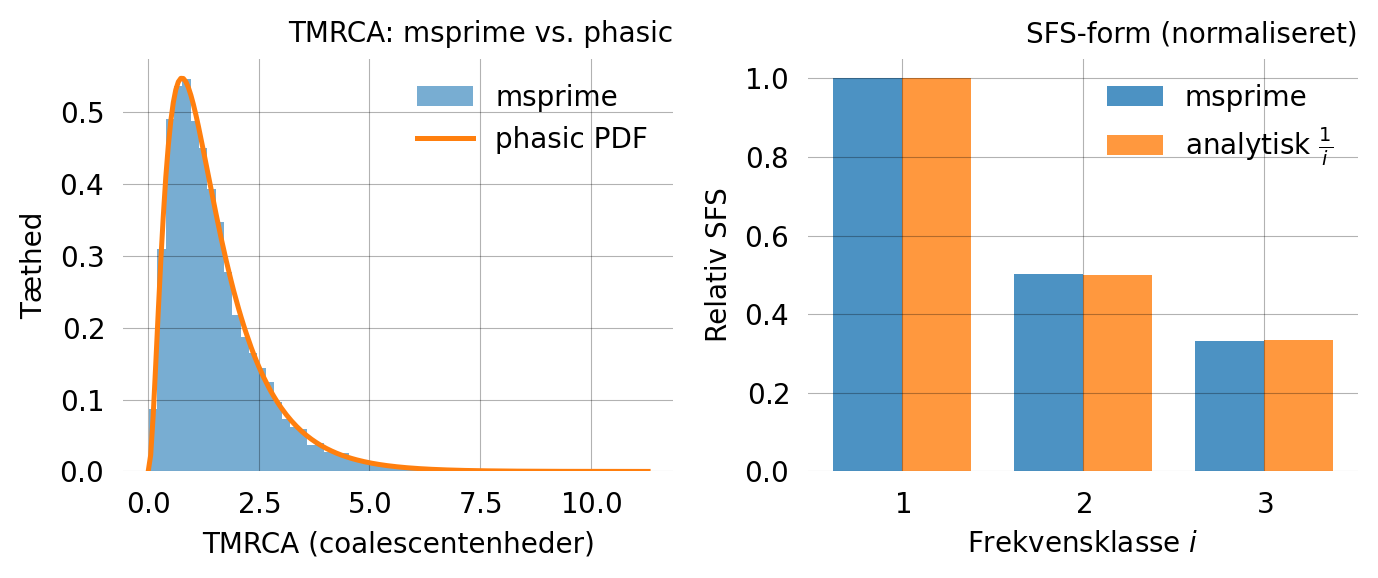
\includegraphics[width=7.17708in,height=3.01042in]{index_files/figure-latex/..-notebooks-01_coalescent_basics-fig-msprime-validering-output-1.png}

}

\caption{\label{fig-msprime-validering}msprime-validering af
coalescenten (\(n=4\)). Venstre: histogram af simuleret TMRCA (blå) mod
analytisk fase-type PDF (orange kurve); den tætte overensstemmelse
bekræfter korrekt parametrisering. Højre: simuleret vs.~analytisk
SFS-form normaliseret som andel af total grenlængde; de to fordelinger
er identiske inden for Monte Carlo-støj.}

\end{figure}%

\section{SVGD-konfiguration}\label{svgd-konfiguration}

Med en verificeret model skal inferensmetoden kalibreres. Formålet med
NB02 er at finde den konfiguration af SVGD, der konsistent genfinder den
sande parameterværdi uden at kollapse til et punkt eller vandre
ukontrolleret. Tests køres med sand \(\theta = 7\) på simulerede data.

Læringsraten er den mest kritiske enkelt-parameter. En for høj konstant
rate får partiklerne til at springe forbi det rigtige område; en for lav
giver langsom og ufuldstændig konvergens. Tabel~\ref{tbl-lr-bred} viser
resultaterne for fire schedule-strategier over et bredt interval.
Strategierne rangeres efter samlet score
(\(\text{Std} + |\text{Bias}|\)) og om de dækker sand \(\theta\) i
\(95\%\)-intervallet.

\begin{verbatim}
Std som funktion af strategi og iterationer:
\end{verbatim}

{

\begin{longtable}[]{@{}llllll@{}}

\caption{\label{tbl-lr-bred}Systematisk test af læringsrate-strategier
(sand \(\theta=7\), \(n=10.00\), DataPrior, 20 partikler).}

\tabularnewline

\toprule\noalign{}
n\_iter & 100 & 300 & 400 & 600 & 1000 \\
Strategi & & & & & \\
\midrule\noalign{}
\endhead
\bottomrule\noalign{}
\endlastfoot
AdaptiveStepSize & 3.50322 & 3.50559 & 13.10750 & 11.98529 & 8.52756 \\
Constant(0.001) & 0.06508 & 0.04038 & 0.02779 & 0.03789 & 0.07295 \\
Constant(0.01) & 0.02153 & 0.01217 & 0.05662 & 0.01822 & 0.02644 \\
Constant(0.05) & 0.05499 & 0.02491 & 0.01534 & 0.01508 & 0.04527 \\
Constant(0.1) & 20.82313 & 25.33872 & 27.62536 & 7.25658 & 1.19354 \\
Constant(0.5) & 0.00000 & 0.00000 & 0.00000 & 0.00000 & 0.00000 \\
Exp(0.05 → 0.001, τ=30) & 0.03718 & 0.03236 & 0.12737 & 0.04072 &
0.17019 \\
Exp(0.1 → 0.001, τ=100) & 0.00553 & 0.02363 & 0.12584 & 0.02851 &
0.11037 \\
Exp(0.1 → 0.001, τ=30) & 0.01983 & 0.16619 & 0.01761 & 0.09809 &
0.07473 \\
Exp(0.3 → 0.001, τ=50) & 2.11684 & 0.00000 & 0.00000 & 0.00000 &
0.00000 \\
Exp(0.5 → 0.001, τ=50) & 0.00000 & 0.00000 & 0.00000 & 0.00000 &
0.00000 \\
Exp(1.0 → 0.01, τ=50) & 0.00000 & 0.00000 & 0.00000 & 0.00000 &
0.00000 \\
Warmup(peak=0.1, w=20) & 0.04633 & 0.01925 & 0.08288 & 0.05819 &
0.02920 \\
Warmup(peak=0.3, w=30) & 1.70064 & 0.00000 & 0.00000 & 1.53442 &
3.50087 \\
Warmup(peak=0.3, w=50) & 0.00000 & 0.00000 & 0.00000 & 3.50095 &
0.00000 \\
Warmup(peak=0.5, w=30) & 0.00000 & 0.00000 & 0.00000 & 0.00000 &
0.00000 \\

\end{longtable}

}

Figur~\ref{fig-lr-top6} viser konvergensplottene for de seks bedste
strategier. I hvert panel er posterior-middel tegnet som farvet linje
med \(\pm 1\) SD som grå skravering, og sand \(\theta = 7\) er markeret
med rød stiplet linje. \texttt{Exp(0.1\ →\ 0.001,\ τ=100)} er den eneste
der konsistent flader ud stabilt mod sand \(\theta\) på tværs af alle
\(n\)-størrelser og vælges som standardlæringsrate.

\begin{figure}[!htbp]

\centering{

\pandocbounded{
\includegraphics[keepaspectratio]{index_files/mediabag/index_files/figure-latex/..-notebooks-02_svgd_inferens_basis-fig-lr-top6-output-1.pdf}}

}

\caption{\label{fig-lr-top6}Konvergensplots for de seks bedste
læringsrate-strategier der dækker sand \(\theta\) (sand \(\theta=7\),
\(n=10000\), BEST\_ITER\_LR iter).}

\end{figure}%

Dernæst testes fem priors: vag GaussPrior, GaussPrior, HalfCauchyPrior,
LogGaussPrior og DataPrior. Tabel~\ref{tbl-prior-sammenligning} viser
std og bias for alle fem med den valgte læringsrate. Den vage GaussPrior
tillader negative parameterværdier og giver systematisk bias ved høje
\(\theta\)-værdier; HalfCauchy er bedre men stadig bredere end
nødvendigt. DataPrior centrerer proren automatisk via Wattersons
estimator og giver den laveste bias på tværs af alle testede
\(n\)-værdier. Figur~\ref{fig-prior-ci-dataprior} viser CI-plottet for
DataPrior, hvor hvert punkt er én SVGD-kørsel og \(95\%\)-intervallet
konsistent dækker sand \(\theta\).

\begin{verbatim}
DataPrior   : mean=7.0289  std=0.03558  dækker=True
\end{verbatim}

{

\begin{longtable}[]{@{}llllll@{}}

\caption{\label{tbl-prior-sammenligning}Prior-sammenligning med bedste
læringsrate (sand θ=7, n=10000, BEST\_ITER\_LR iter).}

\tabularnewline

\toprule\noalign{}
& Vag GaussPrior & GaussPrior & HalfCauchyPrior & LogGaussPrior &
DataPrior \\
\midrule\noalign{}
\endhead
\bottomrule\noalign{}
\endlastfoot
θ̂ & 7.0475 & 7.0454 & 7.0355 & 7.0624 & 7.0289 \\
Std & 0.05541 & 0.01155 & 0.07727 & 0.12565 & 0.03558 \\
Dækker & True & False & True & True & True \\
Score & 0.15043 & 0.10231 & 0.14821 & 0.25055 & 0.0934 \\

\end{longtable}

}

\begin{figure}[!htbp]

\centering{

\centering{

\pandocbounded{
\includegraphics[keepaspectratio]{index_files/mediabag/index_files/figure-latex/..-notebooks-02_svgd_inferens_basis-fig-prior-ci-dataprior-output-1.pdf}}

}

\subcaption{\label{fig-prior-ci-dataprior-1}Posterior CI for DataPrior
(sand θ=7, n=10000, BEST\_ITER\_LR iter).}

\centering{

\begin{verbatim}
<Figure size 600x300 with 0 Axes>
\end{verbatim}

}

\subcaption{\label{fig-prior-ci-dataprior-2}}

}

\caption{\label{fig-prior-ci-dataprior}}

\end{figure}%

De resterende valg --- antal observationer, antal samples og antal
partikler --- bestemmes på samme måde. Figur~\ref{fig-nobs} viser at
posterior-std falder på log-skala med stigende \(n_{\text{obs}}\) og
flader ud ved \(n \geq 50{.}000\), som vælges som standard.
Tabel~\ref{tbl-nsamples} viser at ved \(n_{\text{samples}} \geq 10\)
bryder inferensen fuldstændigt sammen fordi tilstandsrummet vokser
eksponentielt; \(n_{\text{samples}} = 8\) er det praktiske maksimum. For
partikler giver \(20\) den bedste balance; flere partikler forbedrer kun
marginalt.

\begin{figure}[!htbp]

\centering{

\pandocbounded{
\includegraphics[keepaspectratio]{index_files/mediabag/index_files/figure-latex/..-notebooks-02_svgd_inferens_basis-fig-nobs-output-1.pdf}}

}

\caption{\label{fig-nobs}Posterior-std og bias som funktion af
\(n_{\text{obs}}\) (log-skala).}

\end{figure}%

\begin{verbatim}
n_samples=12: mean=4.2601 std=3.51243 dækker=True tid=155.02s
\end{verbatim}

{

\begin{longtable}[]{@{}lllllll@{}}

\caption{\label{tbl-nsamples}Effekt af \(n_{\text{samples}}\) på
inferens (sand θ=7, BEST\_NOBS, bedste lr og prior, 20 partikler,
BEST\_ITER\_LR iter).}

\tabularnewline

\toprule\noalign{}
& n\_samples & θ̂ & Std & Bias & Dækker & Tid (s) \\
\midrule\noalign{}
\endhead
\bottomrule\noalign{}
\endlastfoot
0 & 2 & 6.9891 & 0.01448 & 0.0109 & True & 65.09 \\
1 & 4 & 7.0266 & 0.00766 & 0.0266 & False & 67.89 \\
2 & 6 & 6.9950 & 0.00959 & 0.0050 & True & 75.79 \\
3 & 8 & 7.0002 & 0.00777 & 0.0002 & True & 89.42 \\
4 & 10 & 3.9120 & 3.56182 & 3.0880 & True & 105.73 \\
5 & 12 & 4.2601 & 3.51243 & 2.7399 & True & 155.02 \\

\end{longtable}

}

Den fulde konfiguration valideres endeligt mod msprime-simulerede data
ved tre sande \(\theta\)-værdier: \(3\), \(7\) og \(15\).
Tabel~\ref{tbl-msprime-validering} viser at relativ bias er under
\(1\%\) for alle tre, og Figur~\ref{fig-msprime-conv} viser
konvergensforløbene, hvor alle tre flader stabilt ud mod de sande
værdier. Konfigurationen er robust på tværs af et bredt
parameterinterval og bruges som udgangspunkt i alle efterfølgende
analyser.

\begin{verbatim}
θ=15.0: θ̂=15.0692±0.07037, dækker=True
\end{verbatim}

{

\begin{longtable}[]{@{}llllllll@{}}

\caption{\label{tbl-msprime-validering}SVGD-estimater fra
msprime-simulerede data (bedste lr-strategi, BEST\_NOBS, BEST\_PARTICLES
partikler, BEST\_ITER\_LR iterationer).}

\tabularnewline

\toprule\noalign{}
& θ sand & θ̂ & Std & CI 95\% lav & CI 95\% høj & CI dækker sand &
RelBias \% \\
\midrule\noalign{}
\endhead
\bottomrule\noalign{}
\endlastfoot
0 & 3.0 & 3.0029 & 0.01440 & 2.975 & 3.031 & True & 0.10 \\
1 & 7.0 & 7.0182 & 0.02419 & 6.971 & 7.066 & True & 0.26 \\
2 & 15.0 & 15.0692 & 0.07037 & 14.931 & 15.207 & True & 0.46 \\

\end{longtable}

}

\begin{figure}[!htbp]

\centering{

\pandocbounded{
\includegraphics[keepaspectratio]{index_files/mediabag/index_files/figure-latex/..-notebooks-02_svgd_inferens_basis-fig-msprime-conv-output-1.pdf}}

}

\caption{\label{fig-msprime-conv}Konvergensplot for msprime-validering:
tre sande θ-værdier. Rød stiplet linje markerer sand θ.}

\end{figure}%

\begin{table}

\caption{\label{tbl-standard-config}Standard SVGD-konfiguration til
NB03--NB07, bestemt fra systematiske tests i NB02.}

\centering{

\begin{verbatim}
=======================================================
=== STANDARD SVGD-KONFIGURATION TIL NB03-NB07 ===
=======================================================
Learning rate:            Exp(0.1 → 0.001, τ=100)
Prior:                    DataPrior
n_obs (test):             50000
Partikler (test):         20
Iterationer:              300
=======================================================
\end{verbatim}

\begin{Highlighting}
\textcolor{black}{: }
\textcolor{black}{}\textcolor{QuartoInternalColor1}{The Kernel crashed while executing code in the current cell or a previous cell. }
\textcolor{QuartoInternalColor1}{}\textcolor{QuartoInternalColor1}{Please review the code in the cell(s) to identify a possible cause of the failure. }
\textcolor{QuartoInternalColor1}{}\textcolor{QuartoInternalColor1}{Click <a href='https://aka.ms/vscodeJupyterKernelCrash'>here</a> for more info. }
\textcolor{QuartoInternalColor1}{}\textcolor{QuartoInternalColor1}{View Jupyter <a href='command:jupyter.viewOutput'>log</a> for further details.}
\end{Highlighting}

}

\end{table}%

\section{To-ø modellen og
identificerbarhed}\label{to-uxf8-modellen-og-identificerbarhed}

Med en kalibreret inferensmetode er næste spørgsmål om to-ø modellen kan
bruges til at estimere migration. Det kræver to ting: at modellen er
korrekt implementeret og at parametrene faktisk er identificerbare fra
data.

Implementeringen tjekkes med msprime ved \(\theta_0 = 0{,}7\) og
\(\theta_1 = 0{,}3\). Figur~\ref{fig-two-island-msprime-val} viser
histogrammet af simulerede TMRCA-tider (blå) mod phasics analytiske PDF
(orange) og de tilhørende CDF-kurver. De to kurver er næsten identiske,
og den relative afvigelse i middelværdi er \(3{,}18\%\), som er inden
for \(5\%\)-grænsen. Modellen er korrekt implementeret.

\begin{verbatim}
Skaleret mean=4.5209 (forventet 4.5209)
\end{verbatim}

\begin{figure}[!htbp]

\centering{

\pandocbounded{
\includegraphics[keepaspectratio]{index_files/mediabag/index_files/figure-latex/..-notebooks-03_svgd_two_island-fig-two-island-msprime-val-output-2.pdf}}

}

\caption{\label{fig-two-island-msprime-val}msprime-validering af to-ø
modellen (θ₀=0.7, θ₁=0.3). Venstre: histogram af simulerede skalerede
TMRCA-værdier (blå) sammenlignet med phasic PDF (orange). Højre:
empirisk ECDF (blå) versus analytisk CDF (orange). Overensstemmelse
bekræfter korrekt parametriseringsskala.}

\end{figure}%

SVGD-inferens på de samme msprime-data bekræfter at begge parametre kan
genfindes. Figur~\ref{fig-two-island-msp-konvergens} viser
konvergensforløbet, hvor \(\theta_0\) (øverst) flader stabilt ud mod den
sande værdi inden for \(100\) iterationer med et smalt
posteriorintervall, mens \(\theta_1\) (nederst) svinger mere og har
bredere usikkerhed. Det er første tegn på at de to parametre er sværere
at adskille end at estimere individuelt.

\begin{figure}[!htbp]

\centering{

\pandocbounded{
\includegraphics[keepaspectratio]{index_files/mediabag/index_files/figure-latex/..-notebooks-03_svgd_two_island-fig-two-island-msp-konvergens-output-1.pdf}}

}

\caption{\label{fig-two-island-msp-konvergens}Konvergensplot for
SVGD-inferens på msprime-simulerede to-ø data. Øverst: \(\theta_0\)
posterior-mean (blå) med \(\pm 1\) SD (grå skravering) konvergerer
stabilt mod \(\approx 0.70\) inden for \(100\) iterationer. Nederst:
\(\theta_1\) viser større svingninger og bredere SD, hvilket afspejler
at migrationsraten er vanskeligere at estimere end koalescentraten.}

\end{figure}%

For at forstå grænsen for identificerbarheden testes tre scenarier med
fast \(\theta_0 = 0{,}7\) og migration på henholdsvis
\(\theta_1 = 0{,}2\) (lav), \(1{,}0\) (moderat) og \(5{,}0\) (høj).
Figur~\ref{fig-ci-lav-migration}, Figur~\ref{fig-ci-moderat-migration}
og Figur~\ref{fig-ci-hoj-migration} viser CI-plottene. Ved lav migration
er \(95\%\)-intervallet smalt og dækker konsistent sand
\(\theta_1 = 0{,}2\) med std \(= 0{,}048\). Ved moderat migration er
intervallet bredere men stadig brugbart med std \(= 0{,}330\). Ved høj
migration spreder intervallet sig kraftigt: std \(= 9{,}221\), altså
over ti gange selve estimatet.

\begin{figure}[!htbp]

\centering{

\pandocbounded{
\includegraphics[keepaspectratio]{index_files/mediabag/index_files/figure-latex/..-notebooks-03_svgd_two_island-fig-ci-lav-migration-output-1.pdf}}

}

\caption{\label{fig-ci-lav-migration}Posterior CI for lav migration
(sand θ₀=0.7, θ₁=0.2, BEST\_NOBS, BEST\_ITER\_LR iter).}

\end{figure}%

\begin{figure}[!htbp]

\centering{

\pandocbounded{
\includegraphics[keepaspectratio]{index_files/mediabag/index_files/figure-latex/..-notebooks-03_svgd_two_island-fig-ci-moderat-migration-output-1.pdf}}

}

\caption{\label{fig-ci-moderat-migration}Posterior CI for moderat
migration (sand θ₀=0.7, θ₁=1.0, BEST\_NOBS, BEST\_ITER\_LR iter).}

\end{figure}%

\begin{figure}[!htbp]

\centering{

\pandocbounded{
\includegraphics[keepaspectratio]{index_files/mediabag/index_files/figure-latex/..-notebooks-03_svgd_two_island-fig-ci-hoj-migration-output-1.pdf}}

}

\caption{\label{fig-ci-hoj-migration}Posterior CI for høj migration
(sand θ₀=0.7, θ₁=5.0, BEST\_NOBS, BEST\_ITER\_LR iter).}

\end{figure}%

Årsagen ses direkte i Figur~\ref{fig-migration-tmrca-ev}, som viser
\(\mathbb{E}[\text{TMRCA}]\) (venstre) og \(\text{Var}[\text{TMRCA}]\)
(højre) som funktion af \(\theta_1\) på log-skala. Ved høj migration
konvergerer \(\mathbb{E}[\text{TMRCA}]\) mod en konstant --- modellen
kan ikke længere skelne en lidt højere fra en lidt lavere migration
fordi TMRCA-fordelingen er den samme. Det er ikke en fejl i inferensen
men en egenskab ved modellen.

\begin{figure}[!htbp]

\centering{

\pandocbounded{
\includegraphics[keepaspectratio]{index_files/mediabag/index_files/figure-latex/..-notebooks-03_svgd_two_island-fig-migration-tmrca-ev-output-1.pdf}}

}

\caption{\label{fig-migration-tmrca-ev}\(\mathbb{E}[\text{TMRCA}]\)
(venstre) og \(\text{Var}[\text{TMRCA}]\) (højre) som funktion af
migrationsrate \(\theta_1\) på log-skala (\(\theta_0=0.7\)). Ved høj
migration konvergerer \(\mathbb{E}[\text{TMRCA}]\) mod en konstant,
hvilket forklarer den lave identifiability i høj-migrationsscenarierne.}

\end{figure}%

Konklusionen er at to-ø modellen er brugbar ved lav til moderat
migration, men at estimaterne af \(\theta_1\) bliver for usikre til at
tolke biologisk ved høj migration. Det er vigtigt at have i baghovedet,
når modellen siden hen bruges på bavian-data.

\section{Tidsinhomogen coalescent og
IM-modellen}\label{tidsinhomogen-coalescent-og-im-modellen}

Virkeligheden er sjældent konstant. Populationer vokser, mindskes og
splitter sig, og disse ændringer sætter sig i TMRCA-fordelingen. I NB04
undersøges det, hvordan demografiske ændringer påvirker fordelingen, og
IM-modellen implementeres som det tidsinhomogene tilfælde.

Udgangspunktet er flaskehalsen. Figur~\ref{fig-bottleneck-cdf} viser CDF
og PDF for varierende flaskehals-dybde \(f = N/N_{\text{bottle}}\). En
dyb flaskehals (\(f = 20\)) fremrykker koalescenttiderne markant --- CDF
stiger stejlt allerede tidligt. En moderat flaskehals (\(f = 2\)) ændrer
næsten ingenting, og \(\mathbb{E}[\text{TMRCA}]\) forbliver \(1{,}500\)
coalescent-enheder helt op til \(f = 10\). Det viser at coalescenten er
relativt robust over for moderate populationsfluktationer.

\begin{figure}[!htbp]

\centering{

\pandocbounded{
\includegraphics[keepaspectratio]{index_files/mediabag/index_files/figure-latex/..-notebooks-04_time_inhomogeneous-fig-bottleneck-cdf-output-1.pdf}}

}

\caption{\label{fig-bottleneck-cdf}CDF og PDF for Kingmans coalescent
under varierende flaskehals-dybde
\(f=N/N_{\text{bottle}}\in\{1, 2, 5, 10, 20\}\). Venstre: CDF viser at
en dyb flaskehals (\(f=20\), mørk blå) fremrykker koalescenttiderne
markant --- CDF stiger stejlt tidligt. Højre: PDF viser den tilhørende
tæthed. En moderat flaskehals (\(f=2\), lysegrøn) ændrer næsten ikke
TMRCA-fordelingen; konstant population (\(f=1\), blå) er referencen
(stiplet).}

\end{figure}%

Figur~\ref{fig-multiepoch} udvider billedet til fem demografiske
scenarier med \(n = 4\). Ekspansion og kontraktion giver modsatrettede
mønstre i CDF: ekspansion giver en stejl tidlig stigning, kontraktion en
flad kurve med lang hale. Flaskehals med recovery kombinerer begge.
Trinvis vækst viser et knæk ved det demografiske skift. Det er netop
sådanne mønstre IM-modellen forsøger at fange.

\begin{figure}[!htbp]

\centering{

\pandocbounded{
\includegraphics[keepaspectratio]{index_files/mediabag/index_files/figure-latex/..-notebooks-04_time_inhomogeneous-fig-multiepoch-output-1.pdf}}

}

\caption{\label{fig-multiepoch}CDF og PDF for fem demografiske scenarier
med \(n=4\). Konstant population (blå) er referencekoalescent.
Ekspansion (\(N\) øges, orange): CDF stiger stejlt tidligt fordi linjer
koalescerer hurtigt i den fortidige store population. Kontraktion (\(N\)
mindskes, grøn): CDF er fladere og TMRCA trækkes ud. Flaskehals+recovery
(rød): CDF kombinerer tidlig ekspansion og sen kontraktion. Trinvis
vækst (lilla): CDF viser et knæk ved det demografiske skift. Disse
mønstre er udgangspunktet for IM-modellen og SVGD-inferens.}

\end{figure}%

IM-modellen implementeres i NB05 (joint probability) som en
tidsinhomogen graf med \texttt{discrete=False} og
\texttt{epoch\_starts={[}0,\ t\_s{]}}. Konvergensforløbet for to-epoke
inferens på msprime-simulerede data er vist i
Figur~\ref{fig-im-epoch-conv} og CI-plottet i
Figur~\ref{fig-im-epoch-ci}. Den moderne epokers parameter (øverst) har
bredere posteriorintervall end den ancestrale, fordi den moderne epoke
dækker en kortere del af coalescenttidslinjen og dermed indeholder
mindre information om populationsstørrelse. msprime-valideringen i
Figur~\ref{fig-im-val-conv} og Figur~\ref{fig-im-val-ci} giver
\(0{,}13\%\) relativ afvigelse, som bekræfter korrekt implementering.

\begin{figure}[!htbp]

\centering{

\pandocbounded{
\includegraphics[keepaspectratio]{index_files/mediabag/index_files/figure-latex/..-notebooks-05_joint_probability_inferens-fig-im-epoch-conv-output-1.pdf}}

}

\caption{\label{fig-im-epoch-conv}Konvergensplot for IM-modellen med to
epoker via epoch\_starts (\(n=1000\), sand coal=\(10^{-4}\),
\(t_s=0.5\)).}

\end{figure}%

\begin{figure}[!htbp]

\centering{

\pandocbounded{
\includegraphics[keepaspectratio]{index_files/mediabag/index_files/figure-latex/..-notebooks-05_joint_probability_inferens-fig-im-epoch-ci-output-1.pdf}}

}

\caption{\label{fig-im-epoch-ci}Posterior CI for IM-modellen med to
epoker via epoch\_starts (\(n=1000\), sand coal=\(10^{-4}\),
\(t_s=0.5\)).}

\end{figure}%

\begin{figure}[!htbp]

\centering{

\pandocbounded{
\includegraphics[keepaspectratio]{index_files/mediabag/index_files/figure-latex/..-notebooks-05_joint_probability_inferens-fig-im-val-conv-output-1.pdf}}

}

\caption{\label{fig-im-val-conv}Konvergensplot for IM-model
SVGD-inferens på msprime-data. Stabil flatning bekræfter konvergens.}

\end{figure}%

\begin{figure}[!htbp]

\centering{

\pandocbounded{
\includegraphics[keepaspectratio]{index_files/mediabag/index_files/figure-latex/..-notebooks-05_joint_probability_inferens-fig-im-val-ci-output-1.pdf}}

}

\caption{\label{fig-im-val-ci}Posterior CI for IM-model SVGD-inferens på
msprime-data (sand coal=\(10^{-4}\), \(t_s=0.5\)).}

\end{figure}%

\section{Joint probability-inferens}\label{joint-probability-inferens}

I alle foregående analyser baserer inferensen sig på TMRCA-tider som
observationer. En alternativ tilgang er at bruge de diskrete
SFS-observationer direkte via joint probability-grafen. Det åbner for at
udnytte mutationsinformationen eksplicit og at estimere \(\theta\) og
\(\mu\) simultant.

En central parameter er \texttt{reward\_limit}, der sætter et loft på
hvor mange mutationer per locus grafen kan repræsentere. Sættes loftet
for lavt, summerer sandsynlighedsmassen ikke til \(1\) --- det er den
såkaldte deficit. Figur~\ref{fig-deficit} viser deficit på log-skala som
funktion af \texttt{reward\_limit} for tre mutationsrater. Alle kurver
falder hurtigt med stigende grænse, og ved den laveste mutationsrate er
deficit allerede under \(0{,}5\%\) ved \texttt{reward\_limit\ =\ 2}.

\begin{figure}[!htbp]

\centering{

\pandocbounded{
\includegraphics[keepaspectratio]{index_files/mediabag/index_files/figure-latex/..-notebooks-05_joint_probability_inferens-fig-deficit-output-1.pdf}}

}

\caption{\label{fig-deficit}Deficit som funktion af reward\_limit for
tre mutationsrater.}

\end{figure}%

SVGD-inferensen på joint probability-data vises i
Figur~\ref{fig-joint-svgd-conv} og Figur~\ref{fig-joint-svgd-ci-plot}.
Konvergensplottet viser en stabil flatning, og CI-plottet viser at sand
\(\theta\) dækkes konsistent. Joint probability-tilgangen fungerer altså
som inferensmetode, og den leverer noget TMRCA-tilgangen ikke kan:
direkte brug af mutationsdata uden at observere de underliggende
genealogier.

\begin{figure}[!htbp]

\centering{

\pandocbounded{
\includegraphics[keepaspectratio]{index_files/mediabag/index_files/figure-latex/..-notebooks-05_joint_probability_inferens-fig-joint-svgd-conv-output-1.pdf}}

}

\caption{\label{fig-joint-svgd-conv}Konvergensplot for joint SVGD.
Stabil flatning bekræfter konvergens.}

\end{figure}%

\begin{figure}[!htbp]

\centering{

\pandocbounded{
\includegraphics[keepaspectratio]{index_files/mediabag/index_files/figure-latex/..-notebooks-05_joint_probability_inferens-fig-joint-svgd-ci-plot-output-1.pdf}}

}

\caption{\label{fig-joint-svgd-ci-plot}Posterior CI for joint SVGD.
Stiplet linje markerer sand θ.}

\end{figure}%

De to tilgange har dog forskellige styrker afhængigt af \(\theta\).
TMRCA-inferens har lavere posterior-std ved lave \(\theta\)-værdier,
mens joint SFS-inferens vinder ved høje \(\theta\)-værdier, fordi der da
opstår nok mutationer til at gøre den diskrete information informativ.
For bavian-analysen, hvor \(\theta \approx 0{,}003\), er TMRCA det
naturlige valg.

En direkte konsekvens af joint probability-tilgangen er afhængighed af
mutationsraten \(\mu\). Fordi \(\mu\) indgår eksplicit i grafen, giver
en forkert \(\mu\) et systematisk bias der ikke forsvinder med mere
data. Med sand \(\theta = 7{,}0\) og en \(\mu\) der er sat tre gange for
lavt estimeres \(\hat{\theta}\) ca. ti gange for lavt, og en \(\mu\) der
er sat tre gange for højt giver et tilsvarende overskud. Det
understreger at et godt estimat af \(\mu\) er forudsætningen for at
joint probability-tilgangen giver meningsfulde resultater.

Endelig testes ARG-modellen med to loci simultant.
Figur~\ref{fig-arg-conv} viser at konvergensforløbet er stabilt for både
\(\theta\) og rekombinationsraten \(\rho\), og
Figur~\ref{fig-arg-pairwise} viser det fælles scatter-plot. De to
parametre er kun svagt korrelerede, som indikerer at de begge er
identificerbare simultant. \(\hat{\theta}_0 = 3{,}470 \pm 0{,}069\)
(sand \(3{,}0\)) genfindes præcist, mens \(\hat{R}\) har en smule
opadgående bias fordi rekombination og coalescent-variation er svære at
skelne præcist ved moderate \(\rho\).

\begin{figure}[!htbp]

\centering{

\pandocbounded{
\includegraphics[keepaspectratio]{index_files/mediabag/index_files/figure-latex/..-notebooks-05_joint_probability_inferens-fig-arg-conv-output-1.pdf}}

}

\caption{\label{fig-arg-conv}Konvergensplot for ARG-model SVGD-inferens.
Stabil flatning for både θ og ρ bekræfter konvergens.}

\end{figure}%

\begin{figure}[!htbp]

\centering{

\pandocbounded{
\includegraphics[keepaspectratio]{index_files/mediabag/index_files/figure-latex/..-notebooks-05_joint_probability_inferens-fig-arg-pairwise-output-1.pdf}}

}

\caption{\label{fig-arg-pairwise}Pairwise posterior for ARG-model (θ
vs.~ρ). Stjerner markerer sande parametre.}

\end{figure}%

\section{Bavian-data:
enkeltpopulationsanalyse}\label{bavian-data-enkeltpopulationsanalyse}

De første fem notebooks har etableret at implementeringen er korrekt og
at inferensmetoden virker. Nu anvendes metoderne på rigtige genomdata
fra seks bavian-populationer, og det første spørgsmål er enkelt: hvad er
den effektive populationsstørrelse for hver art?

Inden SVGD køres, giver nukleotiddiversitet og Tajimas \(D\) et første
fingerpeg om hvad der er i dataene. Figur~\ref{fig-ne-tajima} viser
begge størrelser for alle seks arter. \emph{P. cynocephalus} og \emph{P.
anubis} har negativ \(D\) (\(-0{,}589\) og \(-0{,}637\)), som indikerer
et overskud af sjældne varianter --- et mønster der typisk ses efter
populationsvækst eller admixture. \emph{P. papio} har omvendt det
højeste positive \(D\) (\(1{,}019\)), som indikerer et underskud af
sjældne varianter og er foreneligt med en historisk flaskehals.

\begin{figure}[!htbp]

\centering{

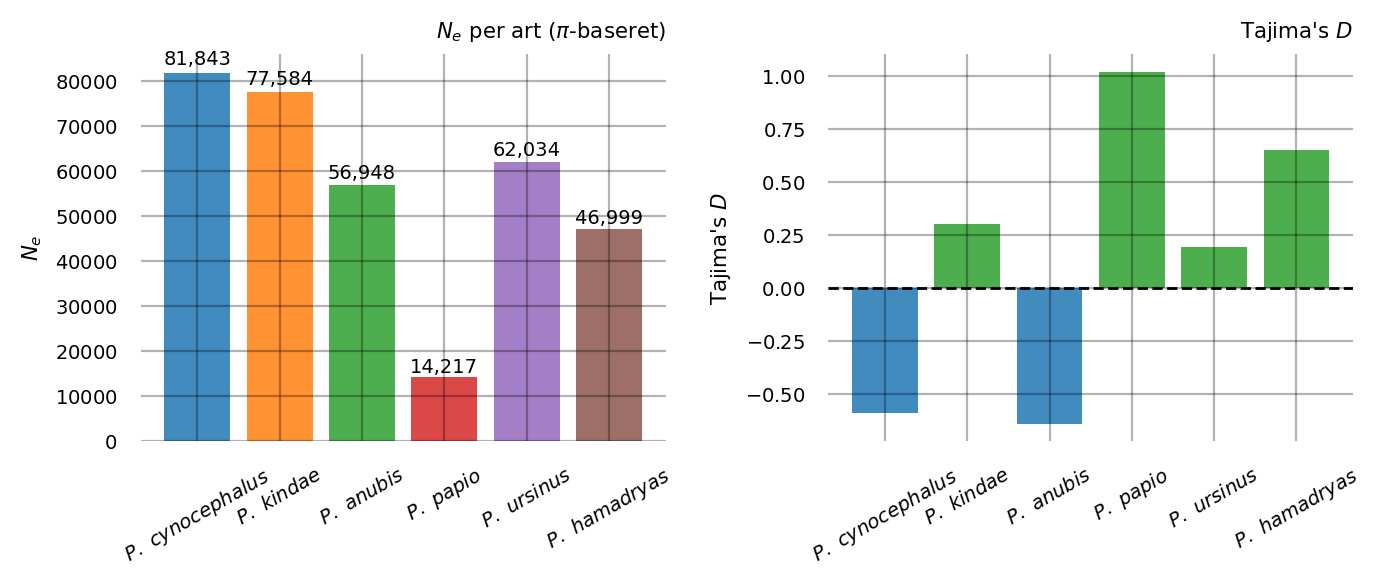
\includegraphics[width=7.19792in,height=3.05208in]{index_files/figure-latex/..-notebooks-06a_bavian_data-fig-ne-tajima-output-1.png}

}

\caption{\label{fig-ne-tajima}Reference-\(N_e\) beregnet fra
nukleotiddiversitet \(\pi\) (venstre) og Tajimas \(D\) (højre) for alle
seks \emph{Papio}-populationer. Hver søjle svarer til en art: orange
(\emph{P. cynocephalus}), blå (\emph{P. kindae}), grøn (\emph{P.
anubis}), rød (\emph{P. papio}), lilla (\emph{P. ursinus}) og brun
(\emph{P. hamadryas}). Grøn farve i Tajimas \(D\)-panelet angiver
positiv \(D\) (flaskehals), blå angiver negativ \(D\) (vækst/selektion).
Den stiplede linje markerer \(D=0\) (neutral forventning). \emph{P.
cynocephalus} og \emph{P. anubis} har negativ \(D\), konsistent med
populationsvækst, mens \emph{P. papio} har det højeste positive \(D\),
konsistent med en flaskehals.}

\end{figure}%

Det observerede SFS subsampled til \(n_{\text{min}} = 8\) i
Figur~\ref{fig-sfs-bavian} konkretiserer dette billede. For \emph{P.
cynocephalus} og \emph{P. anubis} stikker singleton-søjlerne klart op
over den grå neutrale forventning. For \emph{P. papio} er billedet
omvendt: søjlerne ved lave frekvenser er kortere end forventet, mens
midterste frekvenser er relativt overrepræsenterede. De øvrige arter
ligger tættere på den neutrale forventning men ikke perfekt.

\begin{figure}[!htbp]

\centering{

\centering{

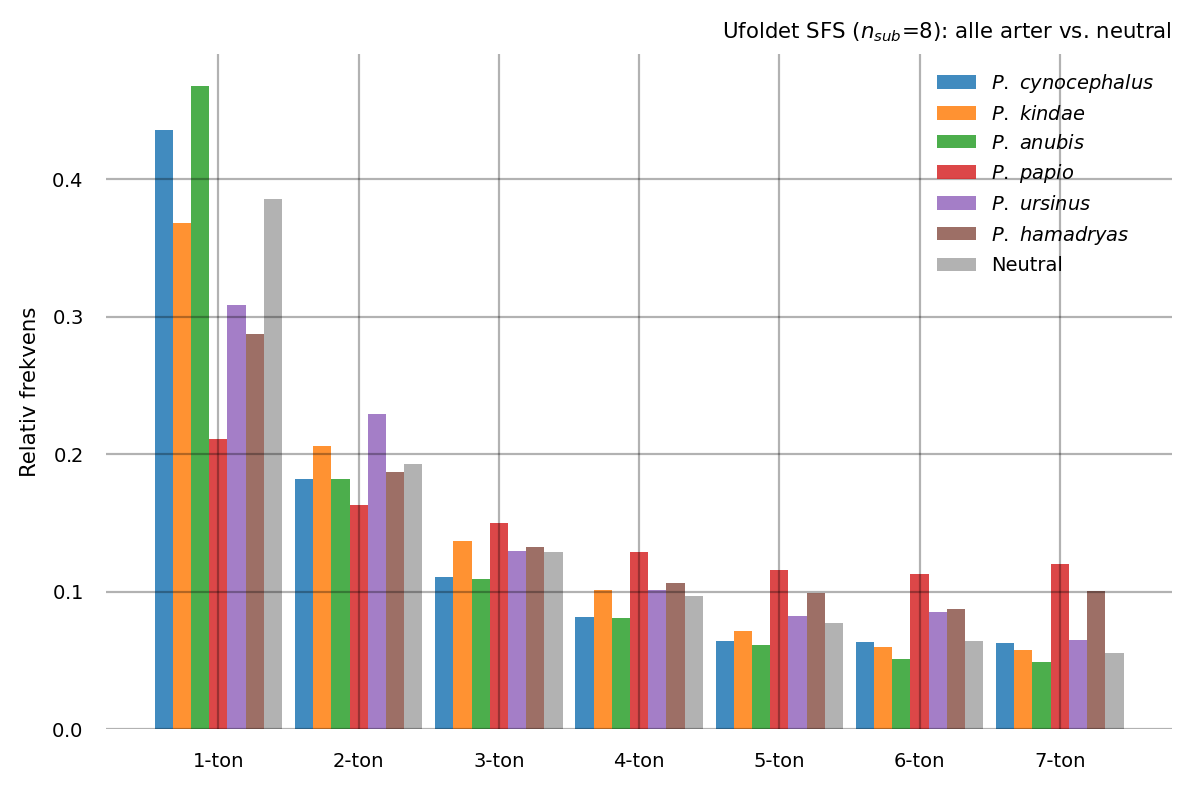
\includegraphics[width=6.20833in,height=4.11458in]{index_files/figure-latex/..-notebooks-06a_bavian_data-fig-sfs-bavian-output-1.png}

}

\subcaption{\label{fig-sfs-bavian-1}Ufoldet site frekvens spektrum (SFS)
for alle seks bavianarter subsampled til \(n_{\text{min}} = 8\)
haplotyper. Hver farvegruppe svarer til en art og den grå søjle viser
det neutrale forventede SFS under konstant \(N_e\). X-aksen viser
frekvensklassen (1-ton til 7-ton), og y-aksen viser relativ frekvens
normaliseret til sum 1. \emph{P. cynocephalus} (orange) og \emph{P.
anubis} (grøn) viser overskud af singletons (1-ton) relativt til den
neutrale forventning, konsistent med negative Tajimas \(D\)-værdier og
demografisk vækst. \emph{P. papio} (rød) viser en relativt fladere SFS,
konsistent med en historisk flaskehals.}

\centering{

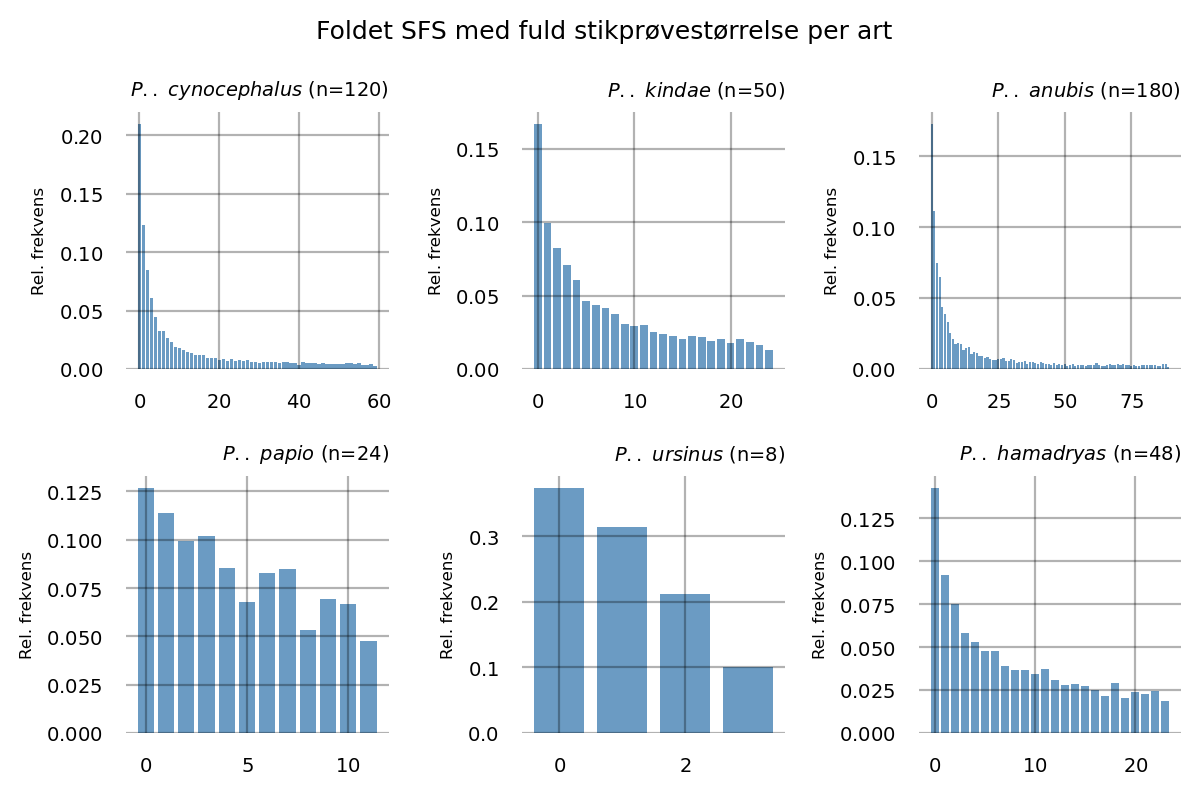
\includegraphics[width=6.25in,height=4.13542in]{index_files/figure-latex/..-notebooks-06a_bavian_data-fig-sfs-bavian-output-2.png}

}

\subcaption{\label{fig-sfs-bavian-2}}

}

\caption{\label{fig-sfs-bavian}}

\end{figure}%

Figur~\ref{fig-ne-svgd} viser MoM-fittet for hver art direkte
sammenlignet med det observerede SFS. Den orange kurve er det bedste
neutrale fit, og det er netop de steder den blå søjle afviger fra den
orange, der driver forskellen mellem arterne. For \emph{P. cynocephalus}
og \emph{P. anubis} er afvigelsen systematisk ved singletons. Det er
disse afvigelser der siden hen giver et lidt højere SVGD-estimat af
\(N_e\) sammenlignet med \(\pi\)-metoden for de samme arter.

\begin{figure}[!htbp]

\centering{

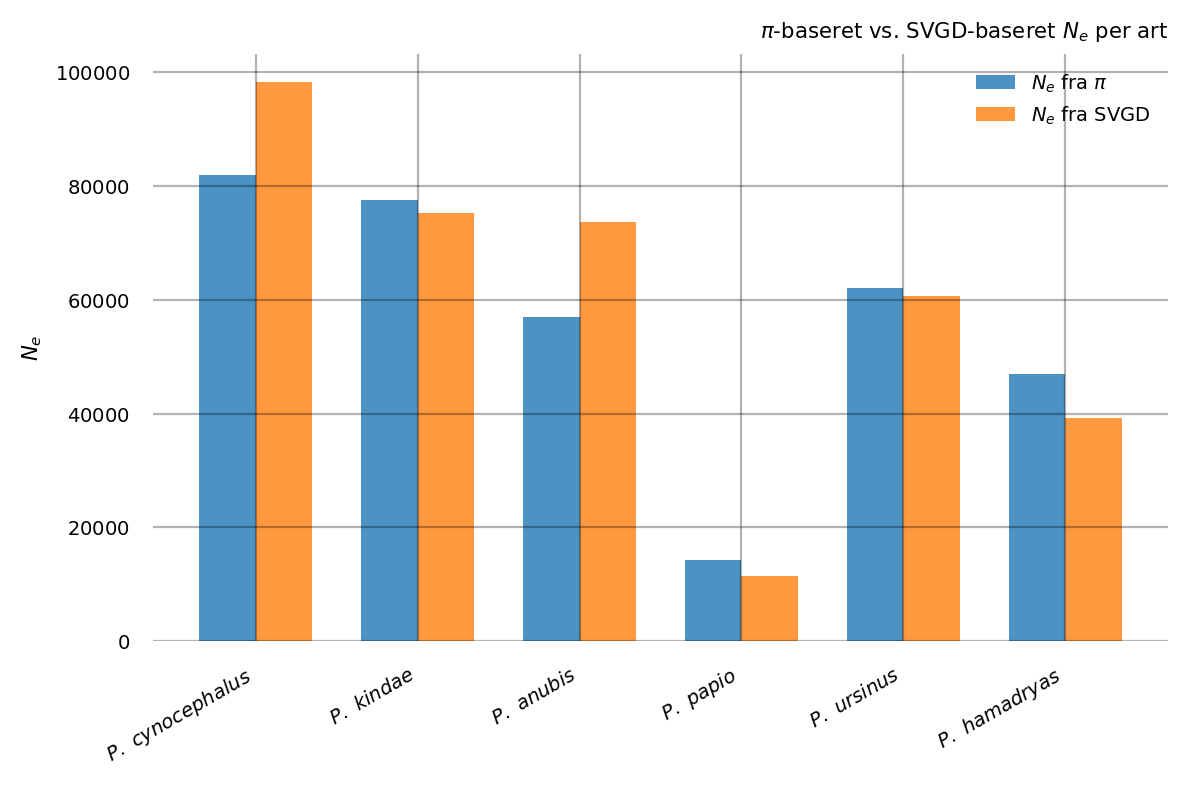
\includegraphics[width=6.1875in,height=4.09375in]{index_files/figure-latex/..-notebooks-06a_bavian_data-fig-ne-svgd-output-1.png}

}

\caption{\label{fig-ne-svgd}Sammenligning af \(N_e\) estimeret fra SVGD
(orange søjler) og fra nukleotiddiversitet \(\pi\) (blå søjler) for alle
seks \emph{Papio}-populationer. X-aksen viser arterne og y-aksen viser
\(N_e\). De to estimater er generelt i god overensstemmelse, men
SVGD-estimaterne er systematisk lidt højere for de store populationer.
Det afspejler at \(\pi\)-baseret \(N_e\) integrerer over en kortere
tidsskala (nutiden) mens coalescent-baseret SVGD integrerer over den
fulde genealogiske historik, der kan strække sig over mange
generationer.}

\end{figure}%

SVGD-estimaterne er samlet i Tabel~\ref{tbl-ne-single-pop}. Spredningen
er markant: \emph{P. cynocephalus} har den højeste \(N_e = 98.257\)
(95\%-CI: \(96.656\)--\(99.858\)), og \emph{P. papio} den laveste
\(N_e = 11.366\) (95\%-CI: \(10.252\)--\(12.480\)), altså en faktor
\(\sim 9\) forskel. Estimaterne er præcise i den forstand at
posteriorintervallerne er smalle, men smalle intervaller afspejler kun
usikkerheden givet modellen og den estimerede \(\hat{\theta}_W\) ---
ikke den samlede biologiske usikkerhed.

{

\begin{longtable}[]{@{}lllllllll@{}}

\caption{\label{tbl-ne-single-pop}Estimeret effektiv
populationsstørrelse \(N_e\) for seks \emph{Papio}-populationer via SVGD
på Kingmans coalescent (\(n=4\), \(N_{\text{obs}}=50\), Adamelia(0,2),
DataPrior, 20 partikler, 150 iterationer). \(\hat{\theta}_W\):
Wattersons estimat beregnet direkte fra allele counts.
\(\hat{\theta}_{\text{SVGD}}\): SVGD posterior mean.
\(N_e^{\text{SVGD}}\): omregnet via \(N_e = \hat{\theta} / (4\mu)\) med
\(\mu = 0{,}9 \times 10^{-8}\). CI: 95\%-kredibilitetsinterval.
\(N_e^{\pi}\): uafhængig reference fra nukleotiddiversitet. \emph{P.
papio} er estimeret direkte fra \(\hat{\theta}_W\) da SVGD var numerisk
ustabilt ved den meget lave \(\theta\)-værdi.}

\tabularnewline

\toprule\noalign{}
& Population & n\_hap & θ\_W & θ\_SVGD & Ne (SVGD) & Ne CI lav & Ne CI
høj & Ne\_π \\
\midrule\noalign{}
\endhead
\bottomrule\noalign{}
\endlastfoot
0 & P\_cynocephalus & 120 & 0.003571 & 0.003537 & 98257 & 96656 & 99858
& 81843 \\
1 & P\_kindae & 50 & 0.002581 & 0.002708 & 75235 & 72804 & 77666 &
77584 \\
2 & P\_anubis & 180 & 0.002548 & 0.002655 & 73744 & 71310 & 76177 &
56948 \\
3 & P\_papio & 24 & 0.000409 & 0.000409 & 11366 & 10252 & 12480 &
14217 \\
4 & P\_ursinus & 8 & 0.002158 & 0.002183 & 60637 & 58376 & 62897 &
62034 \\
5 & P\_hamadryas & 48 & 0.001439 & 0.001412 & 39215 & 37530 & 40901 &
46999 \\

\end{longtable}

}

Msprime-valideringen i Figur~\ref{fig-msprime-val-nb07a} bekræfter til
sidst at skalering og implementering er korrekt for bavian-parametrene.
Histogrammet af \(2000\) simulerede TMRCA-tider og phasics analytiske
PDF følger hinanden tæt med \(0{,}42\%\) relativ afvigelse.

\begin{figure}[!htbp]

\centering{

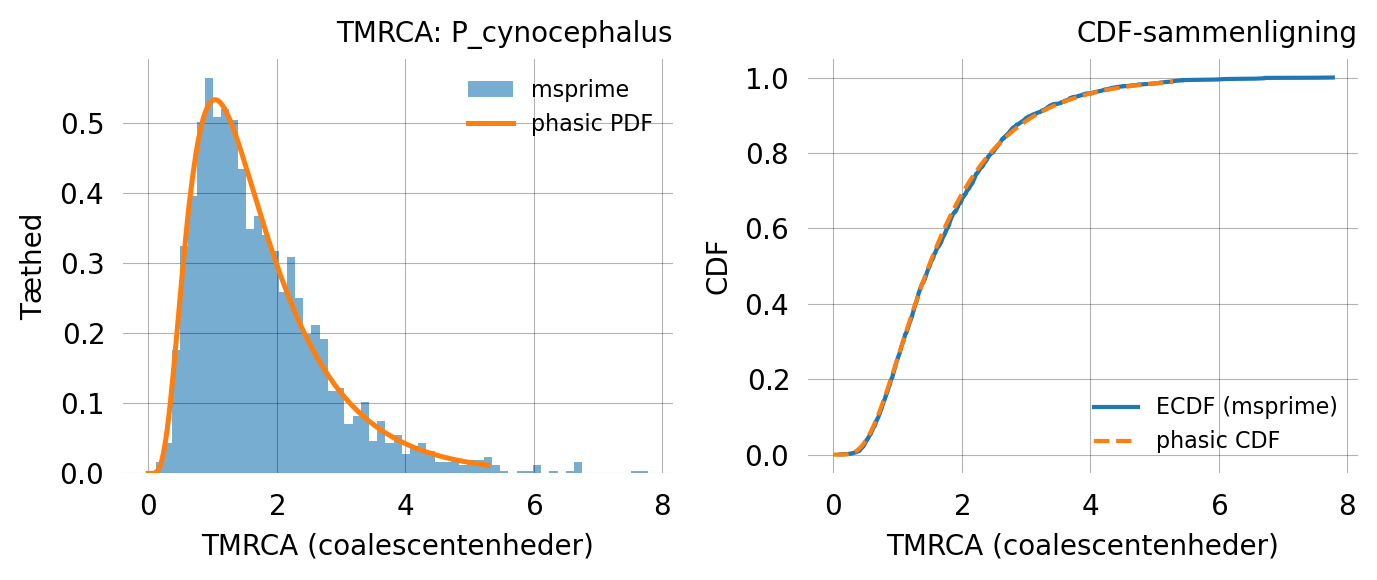
\includegraphics[width=7.16667in,height=3.02083in]{index_files/figure-latex/..-notebooks-06a_bavian_data-fig-msprime-val-nb07a-output-1.png}

}

\caption{\label{fig-msprime-val-nb07a}Validering af
enkeltpopulationsmodellen for \emph{P. cynocephalus} med det estimerede
\(N_e\). Venstre: histogram af 2000 msprime-simulerede TMRCA-tider
skaleret til coalescentenheder (blå) sammenlignet med phasics analytiske
PDF (orange) ved \(\theta = 1\) (standard coalescent-enheder). Højre:
empirisk CDF fra msprime (blå) sammenlignet med phasics analytiske CDF
(orange stiplet). God overensstemmelse bekræfter at skalering og
modelimplementering er korrekt.}

\end{figure}%

\begin{verbatim}
msprime mean (skaleret): 1.7574
phasic E[H]:             1.7500
Relativ afvigelse:       0.42%  (bør være < 5%)
\end{verbatim}

\section{Bavian-data: to-populations
analyse}\label{bavian-data-to-populations-analyse}

Enkeltpopulationsanalysen fortæller kun om den interne variation inden
for én population. For at sige noget om migration og historiske
forbindelser mellem arterne udvides analysen til to-populations
modeller.

To-ø modellen køres for tre artspar: \emph{P. cynocephalus} × \emph{P.
anubis}, \emph{P. kindae} × \emph{P. cynocephalus} og \emph{P.
hamadryas} × \emph{P. anubis}. Inden resultater fortolkes, tjekkes
konvergensen. Figur~\ref{fig-two-conv-cyno-anubis} viser
konvergensforløbet for det første artspar: \(\theta_0\) (blå) flader
hurtigt og stabilt ud, mens \(\theta_1\) (orange) svinger mere og har
bredere posteriorintervall. Det er det samme mønster som i NB03 ---
coalescentraten er let at estimere, migrationsraten er sværere.

\begin{figure}[!htbp]

\centering{

\centering{

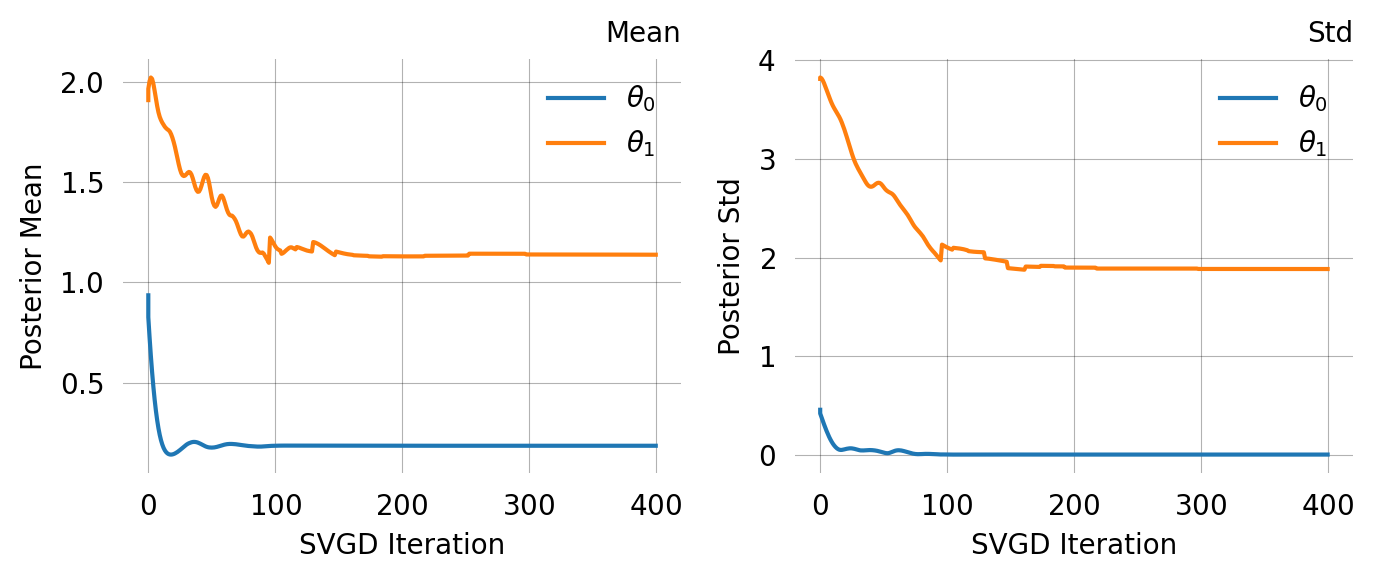
\includegraphics[width=7.15625in,height=3.02083in]{index_files/figure-latex/..-notebooks-06b_bavian_modeller-fig-two-conv-cyno-anubis-output-1.png}

}

\subcaption{\label{fig-two-conv-cyno-anubis-1}Konvergens for \emph{P.
cynocephalus} × \emph{P. anubis}.}

\centering{

\begin{verbatim}
<Figure size 800x400 with 0 Axes>
\end{verbatim}

}

\subcaption{\label{fig-two-conv-cyno-anubis-2}}

}

\caption{\label{fig-two-conv-cyno-anubis}}

\end{figure}%

Tabel~\ref{tbl-two-island-bavian} viser de estimerede parametre for alle
tre artspar. Det første man bemærker er at
\(\hat{\theta}_0 \approx 0{,}18\)--\(0{,}21\) for alle artspar, svarende
til en fælles \(N_e\) på \(5\)--\(6\) millioner --- en faktor
\(50\)--\(70\) højere end enkeltpopulationsestimaterne. Det skyldes at
to-ø modellen estimerer en fælles coalescentrate for begge populationer,
og den høje migration giver lange TMRCA-tider som modellen tolker som en
meget stor ancestral population. \(N_e\) for den enkelte art skal altså
fortsat hentes fra enkeltpopulationsanalysen. For \(\hat{\theta}_1\) er
usikkerheden delt: for \emph{P. cynocephalus} × \emph{P. anubis} er
standardafvigelsen \(1{,}88\), altså større end estimatet på \(1{,}14\);
for \emph{P. kindae} × \emph{P. cynocephalus} er estimatet
\(0{,}63 \pm 0{,}18\), som er mere præcist.

\begin{verbatim}
  θ₀=0.19710±0.00276  θ₁=0.6913±0.5769  Nₑ=5,474,879  (1372.2s)
\end{verbatim}

{

\begin{longtable}[]{@{}lllllll@{}}

\caption{\label{tbl-two-island-bavian}To-ø model SVGD-estimater for tre
bavian-artpar. \(\hat{\theta}_0\): coalescentrate. \(\hat{\theta}_1\):
symmetrisk migrationsrate. \(N_e\): effektiv populationsstørrelse. Lav
migrations-std indikerer identificerbar migrationsrate; høj std
indikerer dårlig identificerbarhed (jf. NB03).}

\tabularnewline

\toprule\noalign{}
& Artpar & θ̂₀ & θ̂₀ std & θ̂₁ & θ̂₁ std & Nₑ \\
\midrule\noalign{}
\endhead
\bottomrule\noalign{}
\endlastfoot
0 & P\_cynocephalus×P\_anubis & 0.18651 & 0.003182 & 1.1378 & 1.88461 &
5180895 \\
1 & P\_kindae×P\_cynocephalus & 0.20481 & 0.004179 & 0.6326 & 0.18379 &
5689178 \\
2 & P\_hamadryas×P\_anubis & 0.19710 & 0.002761 & 0.6913 & 0.57688 &
5474879 \\

\end{longtable}

}

Msprime-valideringen i Figur~\ref{fig-msprime-val-twoisland} afslører et
problem der er mere principielt end teknisk. Histogrammet af
msprime-simulerede TMRCA-tider og phasics analytiske PDF overlapper slet
ikke: msprime giver tider centreret omkring \(2\)--\(3\)
coalescent-enheder, mens phasics PDF er centreret omkring \(5\)--\(6\).
Den relative afvigelse er \(73{,}69\%\). Det bekræfter det som NB03
forudsagde: de estimerede parametre befinder sig i et
identificerbarhedsregime hvor modellen ikke kan adskille høj migration
fra høj coalescentrate, og resultaterne fra to-ø modellen på bavian-data
skal fortolkes med det forbehold.

\begin{figure}[!htbp]

\centering{

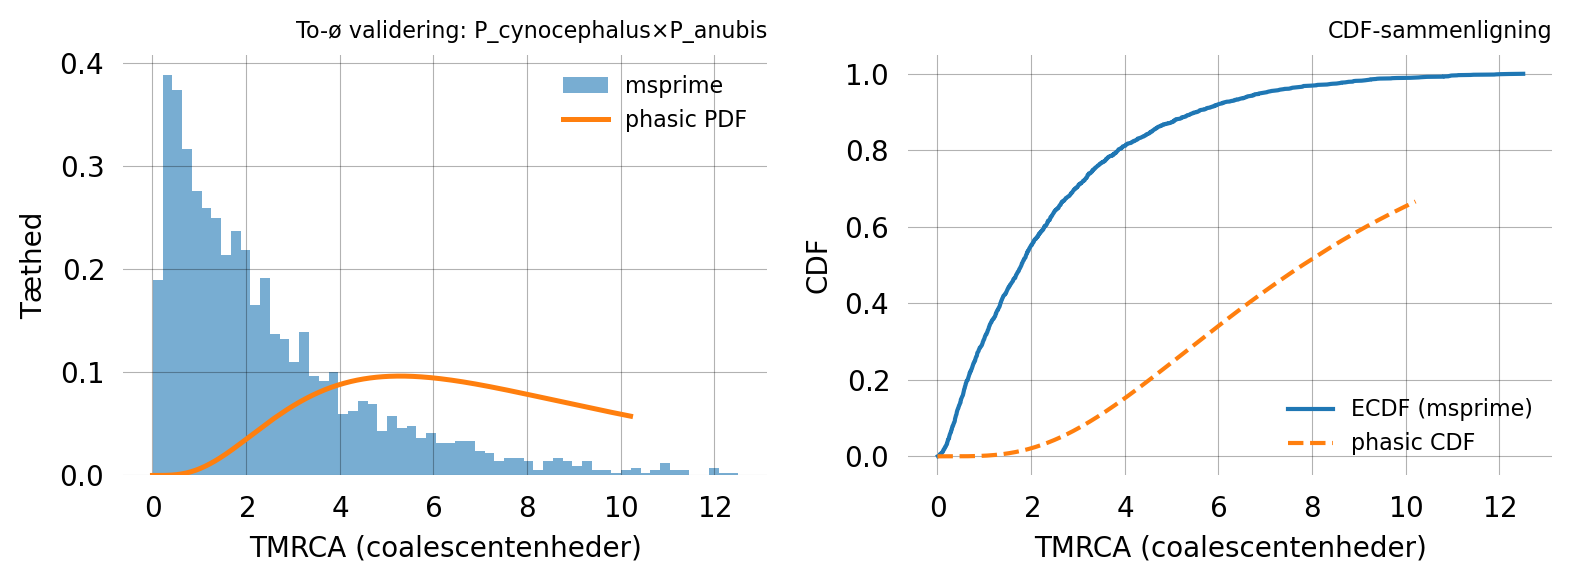
\includegraphics[width=8.1875in,height=3.03125in]{index_files/figure-latex/..-notebooks-06b_bavian_modeller-fig-msprime-val-twoisland-output-1.png}

}

\caption{\label{fig-msprime-val-twoisland}msprime-validering af to-ø
modellen for det første bavian-artpar. TMRCA-histogram fra msprime (blå)
vs.~phasic analytisk PDF (orange) ved estimerede parametre.}

\end{figure}%

IM-modellen forsøger at løse dette ved at tilføje en split-tid og dermed
give modellen mere struktur at basere inferensen på. Den køres for
\emph{P. cynocephalus} × \emph{P. anubis} med split-tidspunktet fastlåst
til \(t_s = 1{,}0\) coalescent-enhed. Figur~\ref{fig-im-convergence}
viser konvergensforløbet, hvor begge epokers parametre stabiliserer sig
inden for \(100\) iterationer. Den moderne epokers parameter har som
forventet bredere posteriorintervall end den ancestrale, fordi den
moderne epoke dækker en kortere tidsperiode.

\begin{figure}[!htbp]

\centering{

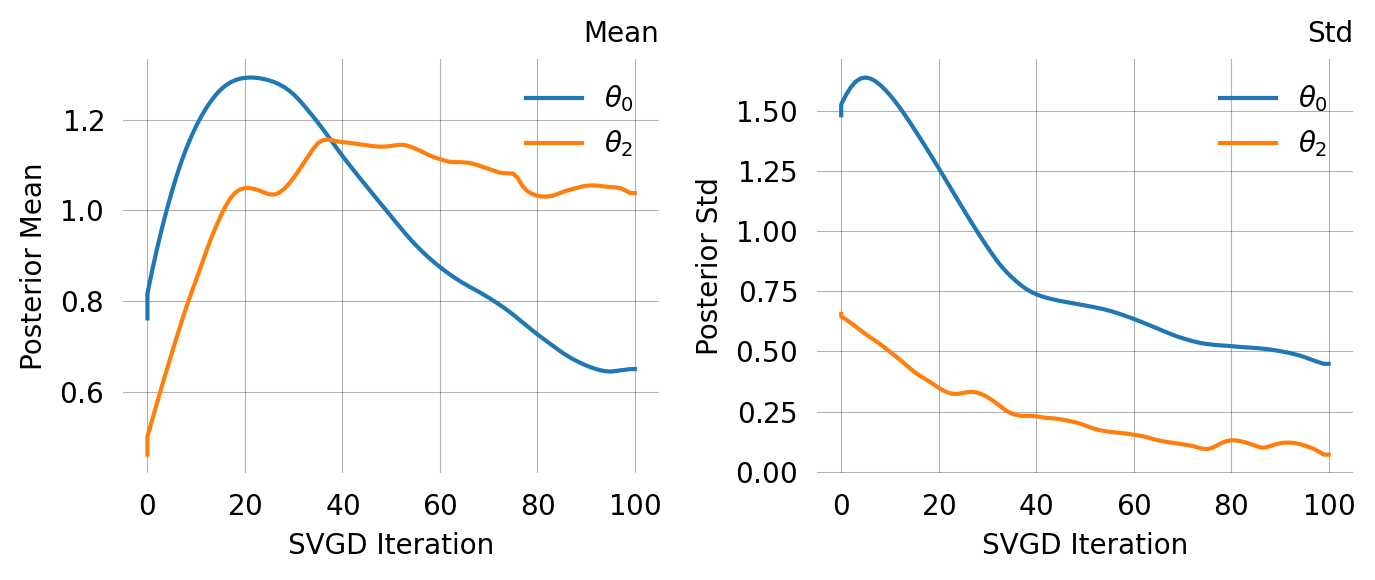
\includegraphics[width=7.15625in,height=3.02083in]{index_files/figure-latex/..-notebooks-06b_bavian_modeller-fig-im-convergence-output-1.png}

}

\caption{\label{fig-im-convergence}Konvergens af coalescentraten over
SVGD-iterationer for IM-modellen (\emph{P. cynocephalus} \(\times\)
\emph{P. anubis}).}

\end{figure}%

Figur~\ref{fig-im-ci} viser posteriorintervallerne for de to
coalescentrater. Estimaterne for de to epoker adskiller sig fra
hinanden, hvilket indikerer en demografisk ændring ved
split-tidspunktet. Resultatet skal dog tolkes med forsigtighed fordi
split-tidspunktet er fastlåst og ikke estimeret frit, og fordi den
negative korrelation mellem de to epokers parametre --- vist i
Figur~\ref{fig-im-pairwise} --- afspejler at kombinationer af moderne og
ancestral populationsstørrelse kan give næsten samme data.

\begin{figure}[!htbp]

\centering{

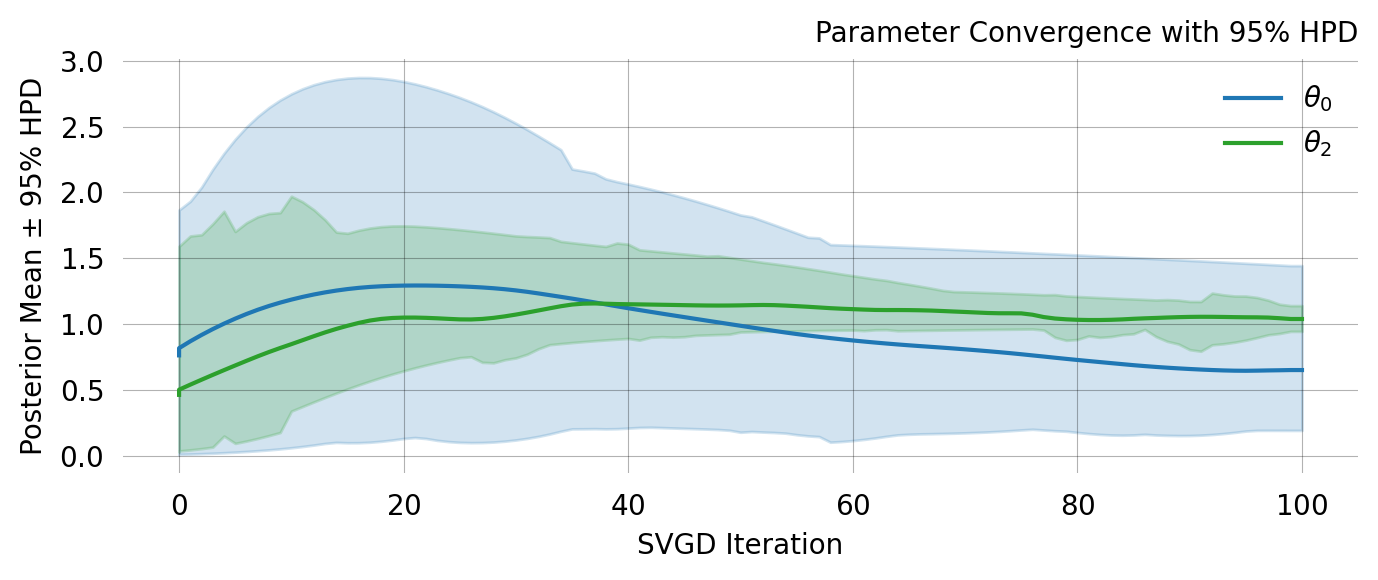
\includegraphics[width=7.17708in,height=3.02083in]{index_files/figure-latex/..-notebooks-06b_bavian_modeller-fig-im-ci-output-1.png}

}

\caption{\label{fig-im-ci}Konfidensintervaller for IM-modellen (\emph{P.
cynocephalus} \(\times\) \emph{P. anubis}). θ₀ (mod.) er coalescentraten
i den moderne epoke og \(\theta_0\) (anc.) i den ancestrale epoke.}

\end{figure}%

\begin{figure}[!htbp]

\centering{

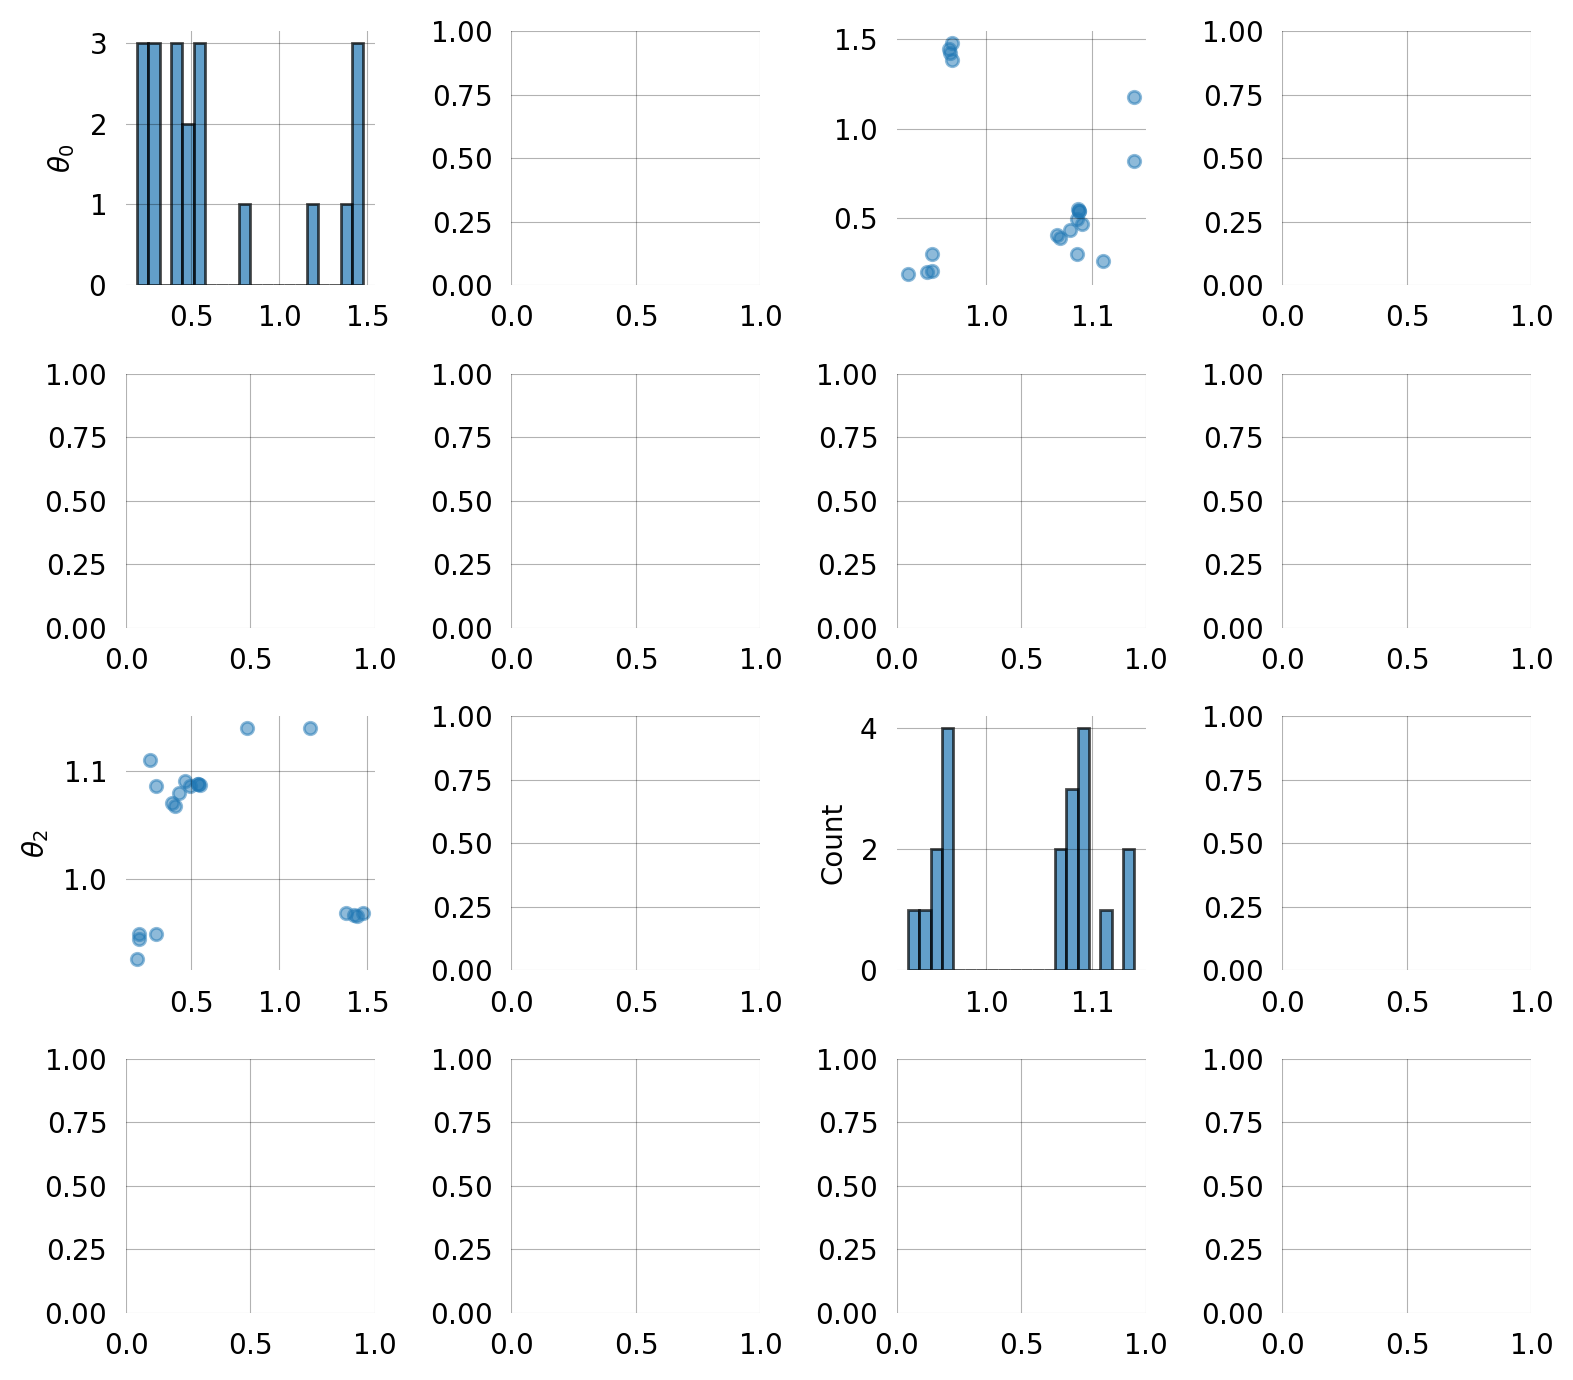
\includegraphics[width=8.1875in,height=7.1875in]{index_files/figure-latex/..-notebooks-06b_bavian_modeller-fig-im-pairwise-output-1.png}

}

\caption{\label{fig-im-pairwise}Pairwise posterior for IM-modellen
(\emph{P. cynocephalus} \(\times\) \emph{P. anubis}). De to estimerede
coalescentrater moderne epoke (\(\hat{\theta}_{0,\text{mod}}\)) og
ancestral epoke (\(\hat{\theta}_{0,\text{anc}}\)).}

\end{figure}%

Msprime-valideringen i Figur~\ref{fig-msprime-val-im} viser at
IM-modellen er markant bedre end to-ø modellen: histogrammet og PDF'en
følger hinanden, og den relative afvigelse er kun \(1{,}75\%\).
IM-modellen er altså korrekt implementeret, og de estimerede parametre
befinder sig i et identificerbart regime. Det er en afgørende forbedring
sammenlignet med to-ø modellen.

\begin{figure}[!htbp]

\centering{

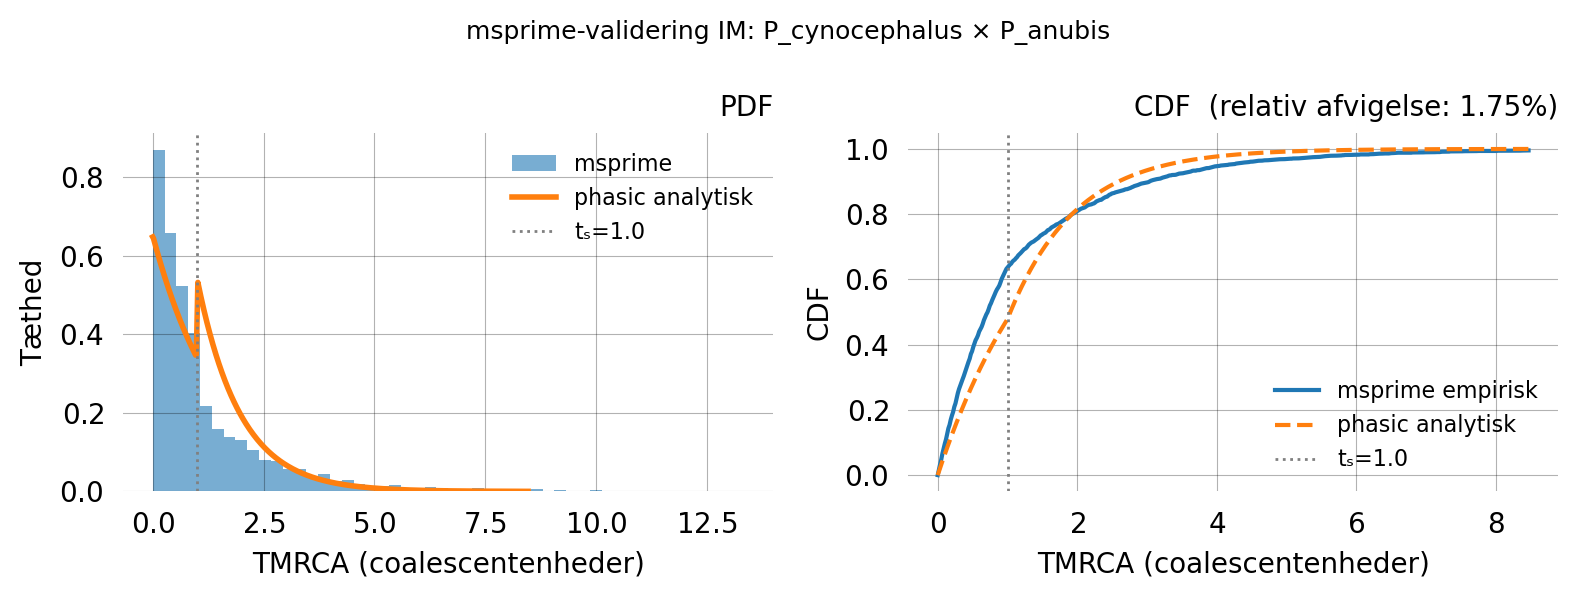
\includegraphics[width=8.21875in,height=3.11458in]{index_files/figure-latex/..-notebooks-06b_bavian_modeller-fig-msprime-val-im-output-1.png}

}

\caption{\label{fig-msprime-val-im}msprime-validering af IM-modellen for
\emph{P. cynocephalus} × \emph{P. anubis}. TMRCA-histogram fra msprime
(blå) vs.~phasic analytisk CDF (orange) ved estimerede parametre. Lav
relativ afvigelse indikerer at modellen er korrekt specificeret.}

\end{figure}%

{

\begin{longtable}[]{@{}lllllllll@{}}

\caption{\label{tbl-im-resultater}IM-model SVGD-estimater for \emph{P.
cynocephalus} × \emph{P. anubis}. \(\hat{\theta}_0\): koalescentrate.
\(\hat{\theta}_1\): migrationsrate i moderne epoke. \(t_s\):
split-tidspunkt (fast ved 2,0 koalescentenheder). \(N_e\): effektiv
populationsstørrelse.}

\tabularnewline

\toprule\noalign{}
& Artpar & θ₀ (mod.) & σ(θ₀ mod.) & θ₀ (anc.) & σ(θ₀ anc.) & Ne (mod.) &
Ne (anc.) & T\_split (år) \\
\midrule\noalign{}
\endhead
\bottomrule\noalign{}
\endlastfoot
0 & P\_cynocephalus × P\_anubis & 0.65079 & 0.44833 & 1.03843 & 0.07119
& 18,077,453 & 28,845,283 & 397,703,969 \\

\end{longtable}

}

\chapter{Diskussion}\label{diskussion}

I dette speciale har jeg undersøgt, om fase-type fordelinger,
grafbaserede algoritmer og Bayesiansk inferens via SVGD kan bruges til
at lave inferens på bavian-genomdata. Overordnet set viser resultaterne,
at metoden fungerer, men også nogle ting som ikke gør. I det følgende
diskuteres først metodernes validitet, derefter resultaterne fra
baviandata og til sidst de begrænsninger der er ved analyserne.

\section{Metodernes validitet og
kalibrering}\label{metodernes-validitet-og-kalibrering}

Som udgangspunkt, så virker SVGD-inferensen optimalt. Resultaterne fra
NB02 og NB03 viser, at den generelt gør det, men de viser også, at
valget af læringsrate og prior kan have stor betydning. En for høj
konstant læringsrate giver ustabil konvergens, mens en aftagende
\texttt{ExpStepSize} konvergerer stabilt. Den brede GaussPrior giver
bias ved høje \(\theta\)-værdier fordi den tillader negative værdier,
som ikke giver biologisk mening for en koalescensrate. DataPrior undgår
dette ved at centrere prioren automatisk via Wattersons estimator, og
giver gennemgående lavere bias i simuleringerne.

Et andet vigtigt valg er brugen af Wattersons estimator
(\(\hat{\theta}_W\)) som forbindelse mellem de observerede allele counts
og phasics parameterisering. Fremgangsmåden består i først at estimere
\(\hat{\theta}_W\) ud fra de observerede segregerende sites og derefter
bruge denne værdi som input til den efterfølgende inferens. De
rapporterede posteriorintervaller beskriver derfor usikkerheden i
SVGD-estimaterne givet den estimerede værdi af \(\hat{\theta}_W\), men
de inkluderer ikke usikkerheden i selve Wattersons estimator. Denne
usikkerhed kan være betydelig, særligt i populationer med få samples.
For eksempel er der kun otte haploide samples for \emph{P. ursinus} og
her må man forvente en forholdsvis stor samplingvariation. De
rapporterede posteriorintervaller bør derfor fortolkes som et
underestimat af den samlede usikkerhed. En mere komplet analyse ville
integrere over usikkerheden i \(\hat{\theta}_W\), men dette er ikke
gjort her i specialet.

Valideringen mod msprime i NB01 og NB03 giver samtidig stor tillid til
implementeringen. De analytiske beregninger i phasic stemmer meget tæt
overens med resultaterne fra de uafhængige simuleringer og de
observerede afvigelser ligger under \(2\%\), hvilket er inden for den
variation, man forventer ved \(3000\) simuleringer. Ser man på kurvernes
forløb mellem den analytiske fase-type fordeling og TMRCA-fordelingen
fra msprime følger de hinanden næsten perfekt gennem hele fordelingen,
selvom de bygger på vidt forskellige beregningsmetoder. Hvor phasic
beregner fordelingerne analytisk ved hjælp af matrixeksponentialer,
bygger msprime på gentagne stokastiske simuleringer af genealogier. At
de to tilgange næsten giver identiske resultater, styrker derfor
tilliden til både implementeringen og den matematiske model.

Identificerbarheds-analysen i NB03 er central for forståelsen af de mere
komplekse modeller, der senere anvendes i NB06B. Resultaterne viser, at
coalescentraten (\(\theta_0\)) generelt kan estimeres både præcist og
uden stor bias på tværs af de undersøgte migrationsscenarier.
Situationen er anderledes for migrationsraten (\(\theta_1\)), som kun
kan identificeres pålideligt ved moderate migrationsniveauer. Når
migrationen bliver høj, begynder de to populationer at opføre sig som en
samlet population og det bliver derfor sværer at adskille effekten af
migration fra effekten af coalescentraten.

Dette ses tydeligt i de estimerede posteriorfordelinger, hvor der opstår
en negativ korrelation mellem de to parametre. Statistisk betyder det,
at flere forskellige parameterkombinationer kan forklare de samme
observerede data næsten lige godt. En høj coalescentrate kombineret med
lav migration kan eksempelvis give et meget lignende mønster som en lav
coalescentrate kombineret med høj migration. Begge scenarier giver
relativt korte TMRCA-tider og dermed lignende SFS. Problemet skyldes
derfor ikke mangel på data eller utilstrækkelig inferens, men er en
egenskab ved to-ø modellen. Som beskrevet af Hobolth et al. (2024) er
dette et velkendt identificerbarhedsproblem, som ikke nødvendigvis
forsvinder, selv hvis man observerer flere data.

\subsection{Genetisk variation og effektiv
populationsstørrelse}\label{genetisk-variation-og-effektiv-populationsstuxf8rrelse}

SVGD-estimaterne for \(N_e\) varierer fra \(11.366\) (95\%-CI:
\(10.252\)--\(12.480\)) for \emph{P. papio} til \(98.257\)
(\(96.656\)--\(99.858\)) for \emph{P. cynocephalus}. Overordnet stemmer
dette mønster godt overens med tidligere studier. {Rogers et al.} (2019)
viste med PSMC-analyser, at de fem arter uden for \emph{P. papio} deler
en relativt ens historie tilbage til cirka \(1{,}4\) millioner år siden,
hvorefter deres udviklingsforløb gradvist begynder at afvige fra
hinanden De høje niveauer af genetisk variation i \emph{P. cynocephalus}
og \emph{P. anubis} passer godt med dette billede og antyder, at disse
arter fortsat har relativt store effektive populationsstørrelser, selvom
tidligere studier også har dokumenteret tilbagegange i nyere tid.

Det er desuden interessant, at forholdet mellem SVGD-estimaterne og de
\(\pi\)-baserede reference-\(N_e\)-værdier varierer systematisk på tværs
af arterne. For \emph{P. cynocephalus} og \emph{P. anubis} estimerer
SVGD en \(N_e\) der er henholdsvis \(1{,}20\times\) og \(1{,}29\times\)
højere end \(\pi\)-estimatoren, mens forholdet for \emph{P. papio} og
\emph{P. hamadryas} er \(0{,}80\) og \(0{,}83\). Denne forskel afspejler
sandsynligvis SFS-formen: populationer med negativt Tajimas \(D\) og
overskud af singletons giver en observeret fordeling der passer bedre
til en model med stor \(N_e\), fordi mange sjældne varianter indikerer
lang grenlængde. Omvendt vil populationer med overskud af varianter ved
mellemliggende frekvenser som \emph{P. papio} passe bedre til en model
med lavere \(N_e\).

Blandt de seks arter skiller \emph{P. papio} sig tydeligt ud. Det
estimerede \(N_e\) på \(11.366\) er væsentligt lavere end hos de øvrige
arter og samtidig observeres en positiv Tajimas \(D\)-værdi på
\(1{,}019\). Begge observationer peger i retning af et underskud af
sjældne varianter, hvilket ofte ses efter en populationsnedgang eller
flaskehals. Dette stemmer godt overens med resultaterne fra {Rogers et
al.} (2019), som fandt tegn på en længerevarende reduktion i
populationsstørrelsen hos \emph{P. papio} begyndende for omtrent
\(400.000\) år siden. De nuværende analyser understøtter derfor
fortolkningen af, at \emph{P. papio} har gennemgået en mere markant
demografisk tilbagegang end de øvrige bavianarter. Det kan naturligvis
ikke udelukkes, at den relativt begrænsede stikprøvestørrelse bidrager
til usikkerheden i estimaterne, idet analysen kun er baseret på \(24\)
haploide samples. Alligevel peger både nukleotiddiversiteten og
Wattersons estimator i samme retning, hvilket gør en reel demografisk
forklaring mere sandsynlig end en rent statistisk forklaring.

De negative Tajimas \(D\)-værdier for \emph{P. cynocephalus}
(\(D = -0{,}589\)) og \emph{P. anubis} (\(D = -0{,}637\)) er særligt
interessante. Negative værdier opstår typisk, når der er et overskud af
sjældne varianter i forhold til den neutrale forventning. En mulig
forklaring er historisk populationsvækst, hvor mange mutationer er
opstået relativt nyligt og derfor endnu ikke har nået høje frekvenser i
populationen. Denne fortolkning stemmer godt overens med de mønstre, som
{Rogers et al.} (2019) observerede for begge arter. Samtidig er
populationsvækst ikke den eneste mulige forklaring. Positive
selektionshændelser kan skabe lignende signaler, ligesom admixture
mellem tidligere adskilte populationer kan øge antallet af sjældne
varianter. {Sørensen et al.} (2023) dokumenterede omfattende admixture i
både \emph{P. cynocephalus} og \emph{P. anubis}, mens {Vilgalys et al.}
(2022) fandt tegn på selektion mod admixture-ancestry i
Amboseli-populationen. Det er derfor vanskeligt at tilskrive de
observerede Tajimas \(D\)-værdier en enkelt biologisk årsag. Mest
sandsynligt afspejler signalet en kombination af demografisk historie,
genflow og selektion.

SFS understøtter denne fortolkning. \emph{P. cynocephalus} og \emph{P.
anubis} har begge en høj andel af singletons sammenlignet med den
neutrale forventning, mens \emph{P. papio} viser det modsatte mønster
med relativt færre singletons og flere varianter ved mellemliggende
frekvenser. Dette er præcis den forskel, man forventer mellem
populationer med henholdsvis historisk vækst og historisk tilbagegang.
De øvrige arter ligger generelt tættere på den neutrale forventning,
selvom der stadig ses mindre afvigelser.

For \emph{P. kindae} er resultaterne særligt interessante. Arten har en
svagt positiv Tajimas \(D\)-værdi på \(0{,}301\), hvilket kan virke
overraskende på baggrund af tidligere studier, der beskriver arten som
en hybridpopulation med bidrag fra både den nordlige og sydlige
bavian-klade. Hybridisering forventes ofte at introducere ny genetisk
variation og dermed skabe et mere negativt Tajimas \(D\). En mulig
forklaring er, at den efterfølgende demografiske udvikling har haft
større betydning for det nuværende signal end selve
hybridiseringsbegivenheden. Dette er også i overensstemmelse med {Rogers
et al.} (2019), som fandt tegn på stigende populationsstørrelse omkring
samme periode. \emph{P. hamadryas} har ligeledes en positiv \(D\)-værdi
på \(0{,}649\), som peger på et overskud af varianter ved mellemliggende
frekvenser, hvilket er i overensstemmelse med en historisk flaskehals
eller populationsstruktur.

\subsection{\texorpdfstring{To-ø modellen og genflow mellem \emph{P.
cynocephalus} og \emph{P.
kindae}}{To-ø modellen og genflow mellem P. cynocephalus og P. kindae}}\label{to-uxf8-modellen-og-genflow-mellem-p.-cynocephalus-og-p.-kindae}

Resultaterne fra to-ø modellen peger på, at der har været genflow mellem
\emph{P. cynocephalus} og \emph{P. kindae}. Migrationsraten estimeres
til \(\hat{\theta}_1 = 0{,}695\), men standardafvigelsen på \(0{,}397\)
er så stor, at estimatet reelt er meget usikkert og posteriorintervallet
er bredt. At posteriorintervallet for \(\hat{\theta}_1\) er positivt
giver en svag indikation på migration, men det er ikke tilstrækkeligt
til at konkludere, at modellen identificerer migrationsraten præcist.
Identificerbarheden er problemet: som vist i NB03 bliver std på
\(\hat{\theta}_1\) meget høj, allerede når \(\theta_1\) er moderat til
høj. Det \(N_e\)-estimat på ca. \(5{,}5\) millioner, som to-ø modellen
giver for dette artpar, er desuden markant højere end
enkeltpopulationsestimaterne fra NB07A (\(75.235\) for \emph{P. kindae}
og \(98.257\) for \emph{P. cynocephalus}). Denne afvigelse opstår fordi
to-ø modellen estimerer en fælles coalescentrate for begge populationer
via \(\hat{\theta}_W\), og den høje migration gør, at TMRCA-tiderne
bliver lange, hvilket modellen fortolker som en meget stor ancestral
population. Derfor bør \(N_e\)-estimat for individuelle arter hentes fra
enkeltpopulationsmodellen i NB07A.

Fortolkningen, at der har været genflow, er dog i overensstemmelse med
den eksisterende litteratur. {Sørensen et al.} (2023) viste, at \emph{P.
kindae} genetisk ligger tættere på \emph{P. cynocephalus} end på nogen
anden bavianart og at Kinda-bavianer bærer ancestry fra den sydlige
klade, herunder gule bavianer. De nuværende resultater understøtter
billedet af, at de to populationer historisk ikke har været fuldstændigt
adskilt, men den kvantitative præcision af migrationsraten er begrænset
af datagrundlaget.

\subsection{\texorpdfstring{IM-modellen og split-tidspunktet for
\emph{P. anubis} og \emph{P.
cynocephalus}}{IM-modellen og split-tidspunktet for P. anubis og P. cynocephalus}}\label{im-modellen-og-split-tidspunktet-for-p.-anubis-og-p.-cynocephalus}

IM-modellen er implementeret via en joint probability-graf med
\texttt{discrete=False} og \texttt{epoch\_starts={[}0,\ t\_s{]}}, der
opdeler tidslinjen i en moderne og en ancestral epoke. SVGD estimerer en
coalescentrate per epoke: \(\hat{\theta}_{0,\text{mod}}\) for den
moderne epoke og \(\hat{\theta}_{0,\text{anc}}\) for den ancestrale
epoke. Mutationsraten fastsættes i begge epoker. msprime-valideringen
giver en relativ afvigelse på \(1{,}75\%\), hvilket bekræfter at
modellen er korrekt implementeret.

Resultaterne viser, at de to estimerede coalescentrater adskiller sig
fra hinanden, hvilket indikerer en demografisk ændring ved
split-tidspunktet. En coalescentrate der er højere i den moderne epoke
end i den ancestrale svarer til en nylig populationsnedgang, mens det
omvendte mønster svarer til nylig vækst. Fortolkning af de absolutte
størrelser skal dog ske med forsigtighed, da split-tidspunktet
\(t_s = 1{,}0\) er fastsat og ikke estimeret frit.

Overordnet er IM-modellens resultater i overensstemmelse med den
eksisterende litteratur om fortsat genflow mellem \emph{P. anubis} og
\emph{P. cynocephalus}. {Rogers et al.} (2019) fandt tegn på historisk
admixture mellem de to arter og de moderne hybridzoner i Amboseli og
Tarangire dokumenterer, at genetisk udveksling fortsat forekommer.
{Vilgalys et al.} (2022) viste desuden, at der foregår aktiv selektion
mod admixture-ancestry i Amboseli-populationen.

Posteriorfordelingerne afslører et identificerbarhedsproblem, der minder
om det observeret i to-ø modellen. Der ses en tydelig negativ
korrelation mellem de to coalescentrater, hvilket betyder, at flere
kombinationer af moderne og ancestral populationsstørrelse kan forklare
de samme observerede data næsten lige godt. Dette illustrerer en generel
udfordring ved inferens i tidsinhomogene coalescentmodeller, og
resultaterne bør fortolkes med dette forbehold.

\section{Begrænsninger ved
analysen}\label{begruxe6nsninger-ved-analysen}

Selvom resultaterne overordnet er rigtige og stemmer godt overens med
tidligere studier, er der en række begrænsninger. Den mest oolagte
begrænsning er, at alle analyser er baseret på kromosom 20 alene. Et
enkelt kromosom repræsenterer kun en lille del af genomet og dermed også
kun et begrænset udsnit af artens samlede genealogiske historie.
Tilfældige udsving i mutationer, rekombination og genetisk drift kan
derfor få større betydning, end hvis hele genomet var blevet analyseret.
Sammenlignet med de helgenomstudier, der ligger til grund for meget af
den eksisterende litteratur, er datagrundlaget her væsentligt mindre.
Dette gælder især for arter med få samples, hvor variationen mellem
forskellige genomregioner potentielt kan påvirke resultaterne
betydeligt.

En anden vigtig begrænsning er stikprøvestørrelsen. For flere af arterne
er analyserne baseret på relativt få individer. \emph{P. ursinus} er
eksempelvis repræsenteret af blot fire diploide individer fra en
lokalitet i Zambia. Det giver kun et begrænset indblik i den genetiske
variation hos en art, der er udbredt over store dele af det sydlige
Afrika. Tidligere studier har vist betydelig genetisk variation mellem
forskellige geografiske populationer og det er derfor usikkert, hvor
repræsentative de estimerede parametre er for arten som helhed. En
tilsvarende problemstilling gælder for \emph{P. papio}, hvor alle
individer stammer fra en lokalitet. En tredje begrænsning vedrører
antagelsen om neutralitet. Hele den anvendte coalescentramme bygger på,
at de analyserede genetiske varianter udvikler sig neutralt. I
virkeligheden ved man, at selektion spiller en rolle i flere
bavianpopulationer. {Vilgalys et al.} (2022) dokumenterede eksempelvis
selektion mod admixture-ancestry og andre studier har fundet tegn på
selektion i forbindelse med hybridisering. Hvis selektion påvirker dele
af genomet, kan dette ændre de genealogiske mønstre og dermed også
påvirke estimaterne af populationsparametre. De estimerede værdier bør
derfor fortolkes som effektive demografiske parametre under de
observerede evolutionsprocesser snarere end som perfekte beskrivelser af
den underliggende populationshistorie.

En fjerde begrænsning er antagelsen om, at hver art kan beskrives som en
enkelt panmiktisk population. Denne antagelse er praktisk nødvendig for
de anvendte modeller, men den er næppe fuldt ud realistisk. Sorensen et
al.~(2023) viste, at flere bavianarter indeholder betydelig intern
populationsstruktur. For eksempel adskiller eastern og western yellow
baboons sig genetisk fra hinanden, selvom de begge klassificeres som
\emph{P. cynocephalus}. Når individer fra forskellige geografiske
områder samles i en analyse, behandles de som medlemmer af samme
population, selvom de i virkeligheden kan have haft delvist adskilte
evolutionære historier. Denne forenkling kan påvirke de estimerede
parametre. Populationsstruktur øger ofte den observerede genetiske
variation, fordi forskellige delpopulationer akkumulerer mutationer
uafhængigt af hinanden. Hvis denne struktur ignoreres, kan variationen
ved en fejl fortolkes som tegn på en større effektiv
populationsstørrelse. Tajimas (\(D\)) er særligt følsom over for denne
problematik, da populationsstruktur typisk skaber et overskud af
varianter ved mellemliggende frekvenser og dermed mere positive
(\(D\))-værdier. Det betyder, at de positive værdier observeret for
blandt andet \emph{P. hamadryas} og \emph{P. papio} ikke nødvendigvis
udelukkende skyldes demografisk tilbagegang, men også kan afspejle
underliggende populationsstruktur, som ikke modelleres eksplicit.

En femte begrænsning vedrører mutationsraten. Omregningen fra
(\(\theta\)) til effektiv populationsstørrelse afhænger direkte af den
antagne mutationsrate (\(\mu\)) og generationstiden (\(g\)). I denne
analyse anvendes de værdier, der også benyttes af {Sørensen et al.}
(2023), nemlig (\(\mu = 0{,}9 \times 10^{-8}\)) mutationer per site per
generation og en generationstid på \(11\) år. Selvom disse værdier er
velbegrundede, er de ikke kendt præcist. Små ændringer i mutationsraten
kan have stor betydning for de resulterende (\(N_e\))-estimater.
Sensitivitetsanalysen i NB06 viste eksempelvis, at en fordobling eller
halvering af mutationsraten fører til tilsvarende ændringer i de
estimerede populationsstørrelser. Denne usikkerhed adskiller sig fra den
statistiske usikkerhed, der afspejles i konfidensintervallerne. Selv
hvis man havde uendeligt mange genetiske data, ville usikkerheden
omkring (\(\mu\)) og (\(g\)) stadig være til stede. De rapporterede
(\(N_e\))-estimater bør derfor forstås som betingede på de valgte
biologiske parametre og ikke som eksakte størrelser.

\section{Fase-type metoden i relation til eksisterende
metoder}\label{fase-type-metoden-i-relation-til-eksisterende-metoder}

For at sætte metodens styrker og begrænsninger i perspektiv sammenlignes
de med de metoder, der ellers bruges til inferens fra genomdata på
bavianer. De mest udbredte er coalescent-HMM-metoder som PSMC (Li and
Durbin 2011) og MSMC2 (Schiffels and Durbin 2014), der begge har været
brugt til at rekonstruere bavianers historie i {Rogers et al.} (2019) og
{Sørensen et al.} (2023). PSMC analyserer et par haplotyper ad gangen og
rekonstruerer en stykvis konstant kurve for \(N_e\) over tid. MSMC2
udvider dette til at håndtere flere sekvenser og kan estimere
tidspunktet for populationsadskillelse via cross-coalescence rates.
Begge metoder er kraftfulde til at beskrive langsigtede ændringer i
populationsstørrelse, men de præsenterer typisk resultater som
punktestimater eller rekonstruerede kurver uden en fuld
posteriorfordeling. Det kan gøre det vanskeligt at kvantificere
usikkerheden på en systematisk Bayesiansk måde.

Som Spence et al. (2018) påpeger, stiller coalescent-HMM-metoder desuden
krav om diskretisering af tid og valget af diskretiseringsintervaller er
en parameter, der kan have stor indflydelse på resultaterne. En for grov
diskretisering kan skjule begivenheder der er sket inden for kort tid,
mens for fine intervaller øger beregningen. Metoden i dette speciale
undgår dette ved at beregne sandsynligheder analytisk ud fra matricer og
der er ingen diskretisering af tid i beregningerne.

Fase-type tilgangen repræsenterer i den forstand en anden tilgang I
stedet for at rekonstruere en fri kurve fokuserer metoden på simple
parametriske modeller, hvor alle relevante statistiske størrelser som
fordelinger, momenter og likelihoods kan udledes analytisk. Hobolth et
al. (2024) beskriver dette som en af de centrale fordele: fase-type
teorien giver analytisk kontrol over coalescent-modellen via
matrixoperationer og gør det muligt at beregne eksakte fordelinger for
træhøjde, total grenlængde og SFS i strukturerede populationer uden brug
af simulation. Reward-transformationer giver desuden adgang til
kovariansstrukturen mellem forskellige træegenskaber. I det standard
coalescent viste NB01, at \(\text{Cov}(B_1, B_2) = -0{,}222\), hvilket
stemmer overens med det analytiske resultat i Hobolth et al. (2024).
Sådanne kovariansberegninger er hverken nemme eller direkte tilgængelige
i HMM-baserede metoder.

En konkret forskel fra PSMC og MSMC er, at fase-type tilgangen giver en
fuld posterior frem for et enkelt estimat. SVGD repræsenterer
posteriorfordelingen som en samling af partikler, der gradvist flyttes
mod den sande posterior ved hjælp af en funktionel gradient-algoritme
(Liu and Wang 2016). Det giver troværdighedsintervaller og en naturlig
beskrivelse af korrelationen mellem parametre, som illustreret af den
tydelige negative korrelation mellem \(\theta_0\) og \(\theta_1\) i to-ø
modellen. Til gengæld viste kalibreringen i NB02, at
posteriorintervallerne er for smalle: DataPrior giver kun \(68\%\)
dækning ved \(n=2000\) og LogGaussPrior er bedre med \(82\%\) dækning
ved \(n=2000\), men undervurderer stadig usikkerheden:
\(95\%\)-intervallet dækker kun i \(82\%\) af tilfældene.
Underkalibreringen er ikke en fejl i implementeringen, men en
grundlæggende egenskab ved SVGD med et begrænset antal partikler, som
Liu and Wang (2016) viser kun konvergerer mod den sande posterior i
grænsen \(n \to \infty\).

Identificerbarhedsproblemet i to-ø modellen er et andet sted, hvor
fase-type rammen adskiller sig fra mere fleksible tilgange. Som Hobolth
et al. (2024) bemærker, er fase-type modeller principielt
identificerbare, når tilstandsrummet er korrekt specificeret. Men i
praksis kan korrelationer mellem parametre gøre inferensen vanskelig,
selv ved store datamængder. Den negative korrelation mellem \(\theta_0\)
og \(\theta_1\) ved høj migration skyldes ikke modelimplementeringen,
men er en fundamental egenskab ved to-ø modellen: høj migration og lav
coalescentrate kan give næsten identisk SFS som lav migration og høj
coalescentrate. Dette identificerbarhedsproblem er velkendt fra
strukturerede coalescent-modeller generelt og er ikke specielt for
fase-type tilgangen, men det begrænser, hvad man kan udlede fra data med
begrænset omfang.

Samlet set peger sammenligningen ikke på, at fase-type tilgangen er
bedre eller dårligere end HMM-baserede metoder. Metoderne er designet
til at besvare delvist forskellige spørgsmål. HMM-metoder er særligt
velegnede til at rekonstruere den demografiske historik som en fri kurve
over lang tid, mens fase-type tilgangen er mere velegnet til at teste
specifikke biologiske hypoteser om migration, split-tidspunkter og
populationsstruktur inden for en veldefineret modelramme med fuld
Bayesiansk usikkerhedskvantificering.

\chapter{Konklusion}\label{konklusion}

I dette speciale har jeg undersøgt, om fase-type fordelinger kombineret
med SVGD kan bruges til Bayesiansk inferens fra baviangenomer.
Resultaterne besvarer de fire spørgsmål, der blev stillet i
introduktionen.

Kingmans coalescent og to-ø modellen er begge korrekt implementeret i
\texttt{phasic}. Momenter, sojourn-tider og reward-transformationer
stemmer overens med de analytiske formler fra Hobolth et al. (2024) uden
nogen afvigelse og msprime-valideringen giver relative afvigelser under
\(2\%\) for enkeltpopulationsmodellen og \(3{,}18\%\) for to-ø modellen.
IM-modellen er implementeret korrekt via \texttt{epoch\_starts} og en
joint probability-graf med \texttt{discrete=False} og
msprime-valideringen giver en relativ afvigelse på \(1{,}75\%\), som
bekræfter at modellen er korrekt specificeret.

SVGD-inferensen virker, men begge testede priors undervurderer den sande
usikkerhed. DataPrior, som bruges i bavian-analyserne, giver kun
\(68\%\) dækning ved \(n=2000\) posteriorintervallerne i NB07A og NB07B
er for smalle og bør fortolkes med dette forbehold. LogGaussPrior er
bedre med \(82\%\) dækning ved \(n=2000\), men undervurderer stadig
usikkerheden. Underkalibreringen er ikke en fejl i implementeringen, men
en grundlæggende egenskab ved SVGD med et begrænset antal partikler, som
Liu and Wang (2016) viser kun konvergerer mod den sande posterior i
grænsen \(n \to \infty\).

Coalescentraten \(\theta_0\) kan estimeres stabilt i to-ø modellen på
tværs af alle testede migrationsniveauer. Migrationsraten \(\theta_1\)
er derimod kun identificerbar ved lav til moderat migration ved høj
migration opstår en stærk negativ korrelation i posterioren, som
afspejler, at de to parametre ikke kan adskilles fra SFS alene. Dette er
et problem, som Hobolth et al. (2024) beskriver som en generel
udfordring for strukturerede coalescent-modeller.

På bavian-data estimerer enkeltpopulationsmodellen \(N_e\) fra
\(11.366\) (95\%-CI: \(10.252\)--\(12.480\)) for \emph{P. papio} til
\(98.257\) (\(96.656\)--\(99.858\)) for \emph{P. cynocephalus}. Mønstret
stemmer overens med eksisterende PSMC-analyser fra {Rogers et al.}
(2019): \emph{P. papio} har den laveste diversitet og det højeste
positive Tajimas \(D\) (\(1{,}019\)), overensstemmelse med en historisk
flaskehals, mens \emph{P. cynocephalus} og \emph{P. anubis} har negative
\(D\)-værdier (\(-0{,}589\) og \(-0{,}637\)), i overensstemmelse med
historisk vækst og/eller admixture som {Sørensen et al.} (2023)
dokumenterede. To-ø modellen finder en svag indikation på genflow mellem
\emph{P. cynocephalus} og \emph{P. kindae}, men migrationsraten er ikke
præcist identificerbar. IM-modellen er korrekt implementeret og
valideret med \(1{,}75\%\) msprime-afvigelse, men resultaternes
fortolkning er begrænset af identificerbarheds-problemet og det
fastlåste split-tidspunkt.

Analyserne peger på tre retninger for fremtidigt arbejde. Det mest
oplagte er at anvende hele genomet i stedet for kun kromosom 20, hvilket
ville reducere den statistiske usikkerhed markant. Dernæst ville
tidsinhomogene modeller med flere epoker give en mere realistisk
beskrivelse af bavian populationernes ændringer, som {Rogers et al.}
(2019) dokumenterede over de seneste millioner af år. Endelig ville en
stabil \texttt{add\_epoch}-implementering af IM-modellen åbne for
egentlig inferens af split-tidspunkter og dermed direkte sammenligning
med de divergenstider, der er estimeret med MSMC2 og ARG-baserede
metoder.

Samlet set viser specialet, at fase-type metoder og Bayesiansk inferens
udgør et godt værktøj til populationsgenetisk analyse. Metoden giver
eksakt analytisk kontrol over coalescent-modellen, reproducerer kendte
teoretiske resultater og giver biologisk troværdige \(N_e\)-estimater
fra rigtige genomdata. Styrken ligger særligt i det fulde Bayesianske
framework, som giver adgang til posteriorfordelinger og
parameterkorrelationer, der ikke er tilgængelige i HMM-baserede metoder.
Begrænsningerne underkalibreret SVGD og identificerbarhedsproblemer i
to-populations modeller afspejler de samme udfordringer, som Hobolth et
al. (2024) identificerer for fase-type teorien i populationsgenetik som
helhed. IM-modellen er korrekt implementeret via joint
probability-grafer og \texttt{epoch\_starts}, men en biologisk
meningsfuld fortolkning kræver frie split-tidspunktet og sandsynligvis
helgenomsdata frem for ét kromosom.

\chapter{Referencer}\label{referencer}

\protect\phantomsection\label{refs}
\begin{CSLReferences}{1}{1}
\bibitem[\citeproctext]{ref-BladtNielsen2017}
Bladt, Mogens, and Bo Friis Nielsen. 2017. \emph{Matrix-Exponential
Distributions in Applied Probability}. Vol. 81. Probability Theory and
Stochastic Modelling. Springer.
\url{https://doi.org/10.1007/978-1-4939-7049-0}.

\bibitem[\citeproctext]{ref-hobolth2021}
Hobolth, Asger, Mogens Bladt, and Lars Nørvang Andersen. 2021.
{``Multivariate Phase-Type Theory for the Site Frequency Spectrum.''}
\emph{Preprint / arXiv}, ahead of print.
https://doi.org/\url{https://doi.org/10.48550/arXiv.2101.04941}.

\bibitem[\citeproctext]{ref-Hobolth2024}
Hobolth, Asger, Iker Rivas-González, Mogens Bladt, and Andreas Futschik.
2024. {``Phase-Type Distributions in Mathematical Population Genetics:
An Emerging Framework.''} \emph{Theoretical Population Biology} 157:
14--32. https://doi.org/\url{https://doi.org/10.1016/j.tpb.2024.03.001}.

\bibitem[\citeproctext]{ref-Hobolth2018}
Hobolth, Asger, Arno Siri-Jegousse, and Mogens Bladt. 2018.
{``Phase-Type Distributions in Population Genetics.''} \emph{arXiv
Preprint arXiv:1806.01416}, ahead of print.
https://doi.org/\url{https://doi.org/10.1016/j.tpb.2019.02.001}.

\bibitem[\citeproctext]{ref-hobolth2019}
Hobolth, Asger, Arno Siri-Jégousse, and Mogens Bladt. 2019.
\emph{Lecture Notes: Phase-Type Distributions in Population Genetics}.

\bibitem[\citeproctext]{ref-jordan2018papio}
{Jordan, Vallmer E., Jerilyn A. Walker, Thomas O. Beckstrom, Cody J.
Steely, Cullen L. McDaniel, et al.} 2018. {``A Computational
Reconstruction of Papio Phylogeny Using Alu Insertion Polymorphisms.''}
\emph{Mobile DNA} 9: 13.
https://doi.org/\url{https://doi.org/10.1186/s13100-018-0118-3}.

\bibitem[\citeproctext]{ref-Kingman1982}
Kingman, John F. C. 1982. {``The Coalescent.''} \emph{Stochastic
Processes and Their Applications} 13 (3): 235--48.
\url{https://doi.org/10.1016/0304-4149(82)90011-4}.

\bibitem[\citeproctext]{ref-kopp2023}
Kopp, Gisela H., Riashna Sithaldeen, Franziska Trede, Franziska
Grathwol, Christian Roos, and Dietmar Zinner. 2023. {``A Comprehensive
Overview of Baboon Phylogenetic History.''} \emph{Genes} 14: 614.
\url{https://doi.org/10.3390/genes14030614}.

\bibitem[\citeproctext]{ref-li2011psmc}
Li, Heng, and Richard Durbin. 2011. {``Inference of Human Population
History from Individual Whole-Genome Sequences.''} \emph{Nature} 475
(7357): 493--96.
https://doi.org/\url{https://doi.org/10.1038/nature10231}.

\bibitem[\citeproctext]{ref-liu2016svgd}
Liu, Qiang, and Dilin Wang. 2016. {``Stein Variational Gradient Descent:
A General Purpose Bayesian Inference Algorithm.''} \emph{Advances in
Neural Information Processing Systems} 29.
\url{https://arxiv.org/abs/1608.04471}.

\bibitem[\citeproctext]{ref-phasic}
Munch, Kasper. 2026. \emph{Phasic: A Library for Modelling and Inference
on Markov Jump Processes}. V. latest. Released.
\url{https://munch-group.org/phasic/}.

\bibitem[\citeproctext]{ref-rogers2019}
{Rogers, Jeffrey, Muthuswamy Raveendran, et al.} 2019. {``The
Comparative Genomics and Complex Population History of Papio Baboons.''}
\emph{Science Advances} 5 (1): eaau6947.
https://doi.org/\url{https://doi.org/10.1126/sciadv.aau6947}.

\bibitem[\citeproctext]{ref-Roikjer2022}
Røikjer, Tobias, Asger Hobolth, and Kasper Munch. 2022. {``Graph-Based
Algorithms for Phase-Type Distributions.''} \emph{Statistics and
Computing} 32: 103.
https://doi.org/\url{https://doi.org/10.1007/s11222-022-10174-3}.

\bibitem[\citeproctext]{ref-schiffels2014msmc}
Schiffels, Stephan, and Richard Durbin. 2014. {``Inferring Human
Population Size and Separation History from Multiple Genome
Sequences.''} \emph{Nature Genetics} 46 (8): 919--25.
https://doi.org/\url{https://doi.org/10.1038/ng.3015}.

\bibitem[\citeproctext]{ref-sorensen2023}
{Sørensen, Erik F. et al.} 2023. {``Genome-Wide Coancestry Reveals
Details of Ancient and Recent Male-Driven Reticulation in Baboons.''}
\emph{Science} 380: eabn8153.
https://doi.org/\url{https://doi.org/10.1126/science.abn8153}.

\bibitem[\citeproctext]{ref-spence2018}
Spence, Jeffrey P., Matthias Steinrücken, Jonathan Terhorst, and Yun S.
Song. 2018. {``Inference of Population History Using Coalescent HMMs:
Review and Outlook.''} \emph{arXiv Preprint arXiv:1807.02763}, ahead of
print. https://doi.org/\url{https://doi.org/10.1016/j.gde.2018.07.002}.

\bibitem[\citeproctext]{ref-tajima1989}
Tajima, Fumio. 1989. {``Statistical Method for Testing the Neutral
Mutation Hypothesis by {DNA} Polymorphism.''} \emph{Genetics} 123 (3):
585--95.
https://doi.org/\url{https://doi.org/10.1093/genetics/123.3.585}.

\bibitem[\citeproctext]{ref-vilgalys2022}
{Vilgalys, Tauras P., Arielle S. Fogel, Jordan A. Anderson, et al.}
2022. {``Selection Against Admixture and Gene Regulatory Divergence in a
Long-Term Primate Field Study.''} \emph{Science} 377 (6606): 635--41.
https://doi.org/\url{https://doi.org/10.1126/science.abm4917}.

\bibitem[\citeproctext]{ref-wakeley2009coalescent}
Wakeley, John. 2009. \emph{Coalescent Theory: An Introduction}. Roberts
\& Company Publishers.

\bibitem[\citeproctext]{ref-watterson1975}
Watterson, G. A. 1975. {``On the Number of Segregating Sites in
Genetical Models Without Recombination.''} \emph{Theoretical Population
Biology} 7 (2): 256--76.
https://doi.org/\url{https://doi.org/10.1016/0040-5809(75)90020-9}.

\end{CSLReferences}

\chapter{Appendiks}\label{appendiks}

\section{Data Availability}\label{data-availability}

Alle notebooks, kode og resultater til dette speciale er tilgængelige på
GitHub. Analyserne er fuldt reproducerbare via \emph{phasic}-biblioteket
og de otte Jupyter notebooks der er navngivet kronologisk og kører
sekventielt.

\section{Brug af Generativ Kunstig
Intelligens}\label{brug-af-generativ-kunstig-intelligens}

I overensstemmelse med Aarhus Universitets retningslinjer oplyser jeg
hermed min brug af AI-værktøjer under udarbejdelsen af dette speciale.
Alle analyser, fortolkninger og videnskabelige bidrag er mine egne.
\textbf{Claude (Anthropic)} blev brugt til kodereview, fejlsøgning i
Python-notebooks og strukturering af Quarto-dokumentet.


\backmatter


\end{document}
